\documentclass[a4paper]{article}
\usepackage[a4paper,left=3cm,right=2cm,top=2.5cm,bottom=2.5cm]{geometry}
\usepackage{palatino}
\usepackage[colorlinks=true,linkcolor=blue,citecolor=blue]{hyperref}
\usepackage{graphicx}
\usepackage{cp1819t}
\usepackage{subcaption}
\usepackage{adjustbox}
\usepackage{color}
%================= local x=====================================================%
\def\getGif#1{\includegraphics[width=0.3\textwidth]{cp1819t_media/#1.png}}
\let\uk=\emph
\def\aspas#1{``#1"}
%================= lhs2tex=====================================================%
%% ODER: format ==         = "\mathrel{==}"
%% ODER: format /=         = "\neq "
%
%
\makeatletter
\@ifundefined{lhs2tex.lhs2tex.sty.read}%
  {\@namedef{lhs2tex.lhs2tex.sty.read}{}%
   \newcommand\SkipToFmtEnd{}%
   \newcommand\EndFmtInput{}%
   \long\def\SkipToFmtEnd#1\EndFmtInput{}%
  }\SkipToFmtEnd

\newcommand\ReadOnlyOnce[1]{\@ifundefined{#1}{\@namedef{#1}{}}\SkipToFmtEnd}
\usepackage{amstext}
\usepackage{amssymb}
\usepackage{stmaryrd}
\DeclareFontFamily{OT1}{cmtex}{}
\DeclareFontShape{OT1}{cmtex}{m}{n}
  {<5><6><7><8>cmtex8
   <9>cmtex9
   <10><10.95><12><14.4><17.28><20.74><24.88>cmtex10}{}
\DeclareFontShape{OT1}{cmtex}{m}{it}
  {<-> ssub * cmtt/m/it}{}
\newcommand{\texfamily}{\fontfamily{cmtex}\selectfont}
\DeclareFontShape{OT1}{cmtt}{bx}{n}
  {<5><6><7><8>cmtt8
   <9>cmbtt9
   <10><10.95><12><14.4><17.28><20.74><24.88>cmbtt10}{}
\DeclareFontShape{OT1}{cmtex}{bx}{n}
  {<-> ssub * cmtt/bx/n}{}
\newcommand{\tex}[1]{\text{\texfamily#1}}	% NEU

\newcommand{\Sp}{\hskip.33334em\relax}


\newcommand{\Conid}[1]{\mathit{#1}}
\newcommand{\Varid}[1]{\mathit{#1}}
\newcommand{\anonymous}{\kern0.06em \vbox{\hrule\@width.5em}}
\newcommand{\plus}{\mathbin{+\!\!\!+}}
\newcommand{\bind}{\mathbin{>\!\!\!>\mkern-6.7mu=}}
\newcommand{\rbind}{\mathbin{=\mkern-6.7mu<\!\!\!<}}% suggested by Neil Mitchell
\newcommand{\sequ}{\mathbin{>\!\!\!>}}
\renewcommand{\leq}{\leqslant}
\renewcommand{\geq}{\geqslant}
\usepackage{polytable}

%mathindent has to be defined
\@ifundefined{mathindent}%
  {\newdimen\mathindent\mathindent\leftmargini}%
  {}%

\def\resethooks{%
  \global\let\SaveRestoreHook\empty
  \global\let\ColumnHook\empty}
\newcommand*{\savecolumns}[1][default]%
  {\g@addto@macro\SaveRestoreHook{\savecolumns[#1]}}
\newcommand*{\restorecolumns}[1][default]%
  {\g@addto@macro\SaveRestoreHook{\restorecolumns[#1]}}
\newcommand*{\aligncolumn}[2]%
  {\g@addto@macro\ColumnHook{\column{#1}{#2}}}

\resethooks

\newcommand{\onelinecommentchars}{\quad-{}- }
\newcommand{\commentbeginchars}{\enskip\{-}
\newcommand{\commentendchars}{-\}\enskip}

\newcommand{\visiblecomments}{%
  \let\onelinecomment=\onelinecommentchars
  \let\commentbegin=\commentbeginchars
  \let\commentend=\commentendchars}

\newcommand{\invisiblecomments}{%
  \let\onelinecomment=\empty
  \let\commentbegin=\empty
  \let\commentend=\empty}

\visiblecomments

\newlength{\blanklineskip}
\setlength{\blanklineskip}{0.66084ex}

\newcommand{\hsindent}[1]{\quad}% default is fixed indentation
\let\hspre\empty
\let\hspost\empty
\newcommand{\NB}{\textbf{NB}}
\newcommand{\Todo}[1]{$\langle$\textbf{To do:}~#1$\rangle$}

\EndFmtInput
\makeatother
%
%
%
%
%
%
% This package provides two environments suitable to take the place
% of hscode, called "plainhscode" and "arrayhscode". 
%
% The plain environment surrounds each code block by vertical space,
% and it uses \abovedisplayskip and \belowdisplayskip to get spacing
% similar to formulas. Note that if these dimensions are changed,
% the spacing around displayed math formulas changes as well.
% All code is indented using \leftskip.
%
% Changed 19.08.2004 to reflect changes in colorcode. Should work with
% CodeGroup.sty.
%
\ReadOnlyOnce{polycode.fmt}%
\makeatletter

\newcommand{\hsnewpar}[1]%
  {{\parskip=0pt\parindent=0pt\par\vskip #1\noindent}}

% can be used, for instance, to redefine the code size, by setting the
% command to \small or something alike
\newcommand{\hscodestyle}{}

% The command \sethscode can be used to switch the code formatting
% behaviour by mapping the hscode environment in the subst directive
% to a new LaTeX environment.

\newcommand{\sethscode}[1]%
  {\expandafter\let\expandafter\hscode\csname #1\endcsname
   \expandafter\let\expandafter\endhscode\csname end#1\endcsname}

% "compatibility" mode restores the non-polycode.fmt layout.

\newenvironment{compathscode}%
  {\par\noindent
   \advance\leftskip\mathindent
   \hscodestyle
   \let\\=\@normalcr
   \let\hspre\(\let\hspost\)%
   \pboxed}%
  {\endpboxed\)%
   \par\noindent
   \ignorespacesafterend}

\newcommand{\compaths}{\sethscode{compathscode}}

% "plain" mode is the proposed default.
% It should now work with \centering.
% This required some changes. The old version
% is still available for reference as oldplainhscode.

\newenvironment{plainhscode}%
  {\hsnewpar\abovedisplayskip
   \advance\leftskip\mathindent
   \hscodestyle
   \let\hspre\(\let\hspost\)%
   \pboxed}%
  {\endpboxed%
   \hsnewpar\belowdisplayskip
   \ignorespacesafterend}

\newenvironment{oldplainhscode}%
  {\hsnewpar\abovedisplayskip
   \advance\leftskip\mathindent
   \hscodestyle
   \let\\=\@normalcr
   \(\pboxed}%
  {\endpboxed\)%
   \hsnewpar\belowdisplayskip
   \ignorespacesafterend}

% Here, we make plainhscode the default environment.

\newcommand{\plainhs}{\sethscode{plainhscode}}
\newcommand{\oldplainhs}{\sethscode{oldplainhscode}}
\plainhs

% The arrayhscode is like plain, but makes use of polytable's
% parray environment which disallows page breaks in code blocks.

\newenvironment{arrayhscode}%
  {\hsnewpar\abovedisplayskip
   \advance\leftskip\mathindent
   \hscodestyle
   \let\\=\@normalcr
   \(\parray}%
  {\endparray\)%
   \hsnewpar\belowdisplayskip
   \ignorespacesafterend}

\newcommand{\arrayhs}{\sethscode{arrayhscode}}

% The mathhscode environment also makes use of polytable's parray 
% environment. It is supposed to be used only inside math mode 
% (I used it to typeset the type rules in my thesis).

\newenvironment{mathhscode}%
  {\parray}{\endparray}

\newcommand{\mathhs}{\sethscode{mathhscode}}

% texths is similar to mathhs, but works in text mode.

\newenvironment{texthscode}%
  {\(\parray}{\endparray\)}

\newcommand{\texths}{\sethscode{texthscode}}

% The framed environment places code in a framed box.

\def\codeframewidth{\arrayrulewidth}
\RequirePackage{calc}

\newenvironment{framedhscode}%
  {\parskip=\abovedisplayskip\par\noindent
   \hscodestyle
   \arrayrulewidth=\codeframewidth
   \tabular{@{}|p{\linewidth-2\arraycolsep-2\arrayrulewidth-2pt}|@{}}%
   \hline\framedhslinecorrect\\{-1.5ex}%
   \let\endoflinesave=\\
   \let\\=\@normalcr
   \(\pboxed}%
  {\endpboxed\)%
   \framedhslinecorrect\endoflinesave{.5ex}\hline
   \endtabular
   \parskip=\belowdisplayskip\par\noindent
   \ignorespacesafterend}

\newcommand{\framedhslinecorrect}[2]%
  {#1[#2]}

\newcommand{\framedhs}{\sethscode{framedhscode}}

% The inlinehscode environment is an experimental environment
% that can be used to typeset displayed code inline.

\newenvironment{inlinehscode}%
  {\(\def\column##1##2{}%
   \let\>\undefined\let\<\undefined\let\\\undefined
   \newcommand\>[1][]{}\newcommand\<[1][]{}\newcommand\\[1][]{}%
   \def\fromto##1##2##3{##3}%
   \def\nextline{}}{\) }%

\newcommand{\inlinehs}{\sethscode{inlinehscode}}

% The joincode environment is a separate environment that
% can be used to surround and thereby connect multiple code
% blocks.

\newenvironment{joincode}%
  {\let\orighscode=\hscode
   \let\origendhscode=\endhscode
   \def\endhscode{\def\hscode{\endgroup\def\@currenvir{hscode}\\}\begingroup}
   %\let\SaveRestoreHook=\empty
   %\let\ColumnHook=\empty
   %\let\resethooks=\empty
   \orighscode\def\hscode{\endgroup\def\@currenvir{hscode}}}%
  {\origendhscode
   \global\let\hscode=\orighscode
   \global\let\endhscode=\origendhscode}%

\makeatother
\EndFmtInput
%
\def\ana#1{\mathopen{[\!(}#1\mathclose{)\!]}}

%---------------------------------------------------------------------------

\title{
       	    Cálculo de Programas
\\
       	Trabalho Prático
\\
       	MiEI+LCC --- 2018/19
}

\author{
       	\dium
\\
       	Universidade do Minho
}


\date\mydate

\makeindex
\newcommand{\rn}[1]{\textcolor{red}{#1}}
\begin{document}

\maketitle

\begin{center}\large
\begin{tabular}{ll}
\textbf{Grupo} nr. & 105
\\\hline
a83610 & Rui Nuno Borges Cruz Oliveira	
\\
a84475 & Ana Rita Miranda Rosendo 
\\
a85731 & Gonçalo José Azevedo Esteves 
\end{tabular}
\end{center}

\section{Preâmbulo}

A disciplina de \CP\ tem como objectivo principal ensinar
a progra\-mação de computadores como uma disciplina científica. Para isso
parte-se de um repertório de \emph{combinadores} que formam uma álgebra da
programação (conjunto de leis universais e seus corolários) e usam-se esses
combinadores para construir programas \emph{composicionalmente}, isto é,
agregando programas já existentes.
  
Na sequência pedagógica dos planos de estudo dos dois cursos que têm
esta disciplina, restringe-se a aplicação deste método à programação
funcional em \Haskell. Assim, o presente trabalho prático coloca os
alunos perante problemas concretos que deverão ser implementados em
\Haskell.  Há ainda um outro objectivo: o de ensinar a documentar
programas, validá-los, e a produzir textos técnico-científicos de
qualidade.

\section{Documentação} Para cumprir de forma integrada os objectivos
enunciados acima vamos recorrer a uma técnica de programa\-ção dita
``\litp{literária}'' \cite{Kn92}, cujo princípio base é o seguinte:
\begin{quote}\em Um programa e a sua documentação devem coincidir.
\end{quote} Por outras palavras, o código fonte e a documentação de um
programa deverão estar no mesmo ficheiro.

O ficheiro \texttt{cp1819t.pdf} que está a ler é já um exemplo de \litp{programação
literária}: foi gerado a partir do texto fonte \texttt{cp1819t.lhs}\footnote{O
suffixo `lhs' quer dizer \emph{\lhaskell{literate Haskell}}.} que encontrará
no \MaterialPedagogico\ desta disciplina descompactando o ficheiro \texttt{cp1819t.zip}
e executando
\begin{Verbatim}[fontsize=\small]
    $ lhs2TeX cp1819t.lhs > cp1819t.tex
    $ pdflatex cp1819t
\end{Verbatim}
em que \href{https://hackage.haskell.org/package/lhs2tex}{\texttt\LhsToTeX} é
um pre-processador que faz ``pretty printing''
de código Haskell em \Latex\ e que deve desde já instalar executando
\begin{Verbatim}[fontsize=\small]
    $ cabal install lhs2tex
\end{Verbatim}
Por outro lado, o mesmo ficheiro \texttt{cp1819t.lhs} é executável e contém
o ``kit'' básico, escrito em \Haskell, para realizar o trabalho. Basta executar
\begin{Verbatim}[fontsize=\small]
    $ ghci cp1819t.lhs
\end{Verbatim}


\noindent Abra o ficheiro \texttt{cp1819t.lhs} no seu editor de texto preferido
e verifique que assim é: todo o texto que se encontra dentro do ambiente
\begin{quote}\small\tt
\text{\tt \char92{}begin\char123{}code\char125{}}
\\ ... \\
\text{\tt \char92{}end\char123{}code\char125{}}
\end{quote}
vai ser seleccionado pelo \GHCi\ para ser executado.

\section{Como realizar o trabalho}
Este trabalho teórico-prático deve ser realizado por grupos de três alunos.
Os detalhes da avaliação (datas para submissão do relatório e sua defesa
oral) são os que forem publicados na \cp{página da disciplina} na \emph{internet}.

Recomenda-se uma abordagem participativa dos membros do grupo
de trabalho por forma a poderem responder às questões que serão colocadas
na \emph{defesa oral} do relatório.

Em que consiste, então, o \emph{relatório} a que se refere o parágrafo anterior?
É a edição do texto que está a ser lido, preenchendo o anexo \ref{sec:resolucao}
com as respostas. O relatório deverá conter ainda a identificação dos membros
do grupo de trabalho, no local respectivo da folha de rosto.

Para gerar o PDF integral do relatório deve-se ainda correr os comando seguintes,
que actualizam a bibliografia (com \Bibtex) e o índice remissivo (com \Makeindex),
\begin{Verbatim}[fontsize=\small]
    $ bibtex cp1819t.aux
    $ makeindex cp1819t.idx
\end{Verbatim}
e recompilar o texto como acima se indicou. Dever-se-á ainda instalar o utilitário
\QuickCheck,
que ajuda a validar programas em \Haskell\ e a biblioteca \gloss{Gloss} para
geração de gráficos 2D:
\begin{Verbatim}[fontsize=\small]
    $ cabal install QuickCheck gloss
\end{Verbatim}
Para testar uma propriedade \QuickCheck~\ensuremath{\Varid{prop}}, basta invocá-la com o comando:
\begin{tabbing}\tt
~~~~~\char62{}~quickCheck~prop\\
\tt ~~~~~\char43{}\char43{}\char43{}~OK\char44{}~passed~100~tests\char46{}
\end{tabbing}

Qualquer programador tem, na vida real, de ler e analisar (muito!) código
escrito por outros. No anexo \ref{sec:codigo} disponibiliza-se algum
código \Haskell\ relativo aos problemas que se seguem. Esse anexo deverá
ser consultado e analisado à medida que isso for necessário.

\Problema

Um compilador é um programa que traduz uma linguagem dita de
\emph{alto nível} numa linguagem (dita de \emph{baixo nível}) que
seja executável por uma máquina.
Por exemplo, o \gcc{GCC} compila C/C++ em código objecto que
corre numa variedade de arquitecturas.

Compiladores são normalmente programas complexos.
Constam essencialmente de duas partes:
o \emph{analisador sintático} que lê o texto de entrada
(o programa \emph{fonte} a compilar) e cria uma sua representação
interna, estruturada em árvore;
e o \emph{gerador de código} que converte essa representação interna
em código executável.
Note-se que tal representação intermédia pode ser usada para outros fins,
por exemplo,
para gerar uma listagem de qualidade (\uk{pretty print}) do programa fonte.

O projecto de compiladores é um assunto complexo que
será assunto de outras disciplinas.
Neste trabalho pretende-se apenas fazer uma introdução ao assunto,
mostrando como tais programas se podem construir funcionalmente à custa de
cata/ana/hilo-morfismos da linguagem em causa.

Para cumprirmos o nosso objectivo, a linguagem desta questão terá que ser, naturalmente,
muito simples: escolheu-se a das expressões aritméticas com inteiros,
\eg\ \( 1 + 2 \), \( 3 * (4 + 5) \) etc.
Como representação interna adopta-se o seguinte tipo polinomial, igualmente simples:
%
\begin{hscode}\SaveRestoreHook
\column{B}{@{}>{\hspre}l<{\hspost}@{}}%
\column{E}{@{}>{\hspre}l<{\hspost}@{}}%
\>[B]{}\mathbf{data}\;\Conid{Expr}\mathrel{=}\Conid{Num}\;\Conid{Int}\mid \Conid{Bop}\;\Conid{Expr}\;\Conid{Op}\;\Conid{Expr}{}\<[E]%
\\
\>[B]{}\mathbf{data}\;\Conid{Op}\mathrel{=}\Conid{Op}\;\Conid{String}{}\<[E]%
\ColumnHook
\end{hscode}\resethooks

\begin{enumerate}
\item
Escreva as definições dos \{cata, ana e hilo\}-morfismos deste tipo de dados
segundo o método ensinado nesta disciplina (recorde módulos como \eg\ \ensuremath{\fun{BTree} } etc).
\item
Como aplicação do módulo desenvolvido no ponto 1,
defina como \{cata, ana ou hilo\}-morfismo a função seguinte:
\begin{itemize}
\item \ensuremath{\Varid{calcula}\mathbin{::}\Conid{Expr}\to \Conid{Int}} que calcula o valor
de uma expressão;
\begin{propriedade}
O valor zero é um elemento neutro da adição.
\begin{hscode}\SaveRestoreHook
\column{B}{@{}>{\hspre}l<{\hspost}@{}}%
\column{13}{@{}>{\hspre}l<{\hspost}@{}}%
\column{E}{@{}>{\hspre}l<{\hspost}@{}}%
\>[B]{}\Varid{prop\char95 neutro1}\mathbin{::}\Conid{Expr}\to \Conid{Bool}{}\<[E]%
\\
\>[B]{}\Varid{prop\char95 neutro1}\mathrel{=}\Varid{calcula}\comp \Varid{addZero}\equiv\Varid{calcula}\;\mathbf{where}{}\<[E]%
\\
\>[B]{}\hsindent{13}{}\<[13]%
\>[13]{}\Varid{addZero}\;\Varid{e}\mathrel{=}\Conid{Bop}\;(\Conid{Num}\;\mathrm{0})\;(\Conid{Op}\;\text{\tt \char34 +\char34})\;\Varid{e}{}\<[E]%
\\
\>[B]{}\Varid{prop\char95 neutro2}\mathbin{::}\Conid{Expr}\to \Conid{Bool}{}\<[E]%
\\
\>[B]{}\Varid{prop\char95 neutro2}\mathrel{=}\Varid{calcula}\comp \Varid{addZero}\equiv\Varid{calcula}\;\mathbf{where}{}\<[E]%
\\
\>[B]{}\hsindent{13}{}\<[13]%
\>[13]{}\Varid{addZero}\;\Varid{e}\mathrel{=}\Conid{Bop}\;\Varid{e}\;(\Conid{Op}\;\text{\tt \char34 +\char34})\;(\Conid{Num}\;\mathrm{0}){}\<[E]%
\ColumnHook
\end{hscode}\resethooks
\end{propriedade}  
\begin{propriedade}
As operações de soma e multiplicação são comutativas.
\begin{hscode}\SaveRestoreHook
\column{B}{@{}>{\hspre}l<{\hspost}@{}}%
\column{13}{@{}>{\hspre}l<{\hspost}@{}}%
\column{E}{@{}>{\hspre}l<{\hspost}@{}}%
\>[B]{}\Varid{prop\char95 comuta}\mathrel{=}\Varid{calcula}\comp \Varid{mirror}\equiv\Varid{calcula}\;\mathbf{where}{}\<[E]%
\\
\>[B]{}\hsindent{13}{}\<[13]%
\>[13]{}\Varid{mirror}\mathrel{=}\Varid{cataExpr}\;\alt{\Conid{Num}}{\Varid{g2}}{}\<[E]%
\\
\>[B]{}\hsindent{13}{}\<[13]%
\>[13]{}\Varid{g2}\mathrel{=}\uncurry{\uncurry{\Conid{Bop}}}\comp (\Varid{swap}\times\Varid{id})\comp \Varid{assocl}\comp (\Varid{id}\times\Varid{swap}){}\<[E]%
\ColumnHook
\end{hscode}\resethooks
\end{propriedade}  
\end{itemize}
\item
Defina como \{cata, ana ou hilo\}-morfismos as funções
\begin{itemize}
\item \ensuremath{\Varid{compile}\mathbin{::}\Conid{String}\to \Conid{Codigo}} - trata-se do compilador propriamente
      dito. Deverá ser gerado código posfixo para uma máquina elementar
      de \pda{stack}. O tipo \ensuremath{\Conid{Codigo}} pode ser definido à escolha.
      Dão-se a seguir exemplos de comportamentos aceitáveis para esta
      função:
\begin{tabbing}\tt
~Tp4\char62{}~compile~\char34{}2\char43{}4\char34{}\\
\tt ~\char91{}\char34{}PUSH~2\char34{}\char44{}~\char34{}PUSH~4\char34{}\char44{}~\char34{}ADD\char34{}\char93{}\\
\tt ~Tp4\char62{}~compile~\char34{}3\char42{}\char40{}2\char43{}4\char41{}\char34{}\\
\tt ~\char91{}\char34{}PUSH~3\char34{}\char44{}~\char34{}PUSH~2\char34{}\char44{}~\char34{}PUSH~4\char34{}\char44{}~\char34{}ADD\char34{}\char44{}~\char34{}MUL\char34{}\char93{}\\
\tt ~Tp4\char62{}~compile~\char34{}\char40{}3\char42{}2\char41{}\char43{}4\char34{}\\
\tt ~\char91{}\char34{}PUSH~3\char34{}\char44{}~\char34{}PUSH~2\char34{}\char44{}~\char34{}MUL\char34{}\char44{}~\char34{}PUSH~4\char34{}\char44{}~\char34{}ADD\char34{}\char93{}\\
\tt ~Tp4\char62{}~
\end{tabbing}
\item \ensuremath{\Varid{show'}\mathbin{::}\Conid{Expr}\to \Conid{String}} - gera a representação textual
      de uma \ensuremath{\Conid{Expr}} pode encarar-se como o \uk{pretty printer}
      associado ao nosso compilador
\begin{propriedade}
Em anexo, é fornecido o código da função \ensuremath{\Varid{readExp}}, que é ``inversa" da função \ensuremath{\Varid{show'}},
tal como a propriedade seguinte descreve:
\begin{hscode}\SaveRestoreHook
\column{B}{@{}>{\hspre}l<{\hspost}@{}}%
\column{E}{@{}>{\hspre}l<{\hspost}@{}}%
\>[B]{}\Varid{prop\char95 inv}\mathbin{::}\Conid{Expr}\to \Conid{Bool}{}\<[E]%
\\
\>[B]{}\Varid{prop\char95 inv}\mathrel{=}\p1\comp \Varid{head}\comp \Varid{readExp}\comp \Varid{show'}\equiv\Varid{id}{}\<[E]%
\ColumnHook
\end{hscode}\resethooks
\end{propriedade}  
\end{itemize}
%% \item Generalize o tipo |Expr| de forma a admitir operadores
%% unários (\eg\ \(-5\)) e repita os exercícios dos pontos anteriores.
\end{enumerate}

\paragraph{Valorização}
Em anexo é apresentado código \Haskell\ que permite declarar
\ensuremath{\Conid{Expr}} como instância da classe \ensuremath{\Conid{Read}}. Neste contexto,  
\ensuremath{\Varid{read}} pode ser vista como o analisador
sintático do nosso minúsculo compilador de expressões aritméticas.

Analise o código apresentado, corra-o e escreva no seu relatório uma explicação
\textbf{breve} do seu funcionamento, que deverá saber defender aquando da
apresentação oral do relatório.

Exprima ainda o analisador sintático \ensuremath{\Varid{readExp}} como um anamorfismo.

\Problema

Pretende-se neste problema definir uma linguagem gráfica \aspas{brinquedo}
a duas dimensões (2D) capaz de especificar e desenhar agregações de
caixas que contêm informação textual.
Vamos designar essa linguagem por \ensuremath{\Conid{L2D}} e vamos defini-la como um tipo
 em \Haskell:
\begin{hscode}\SaveRestoreHook
\column{B}{@{}>{\hspre}l<{\hspost}@{}}%
\column{E}{@{}>{\hspre}l<{\hspost}@{}}%
\>[B]{}\mathbf{type}\;\Conid{L2D}\mathrel{=}\Conid{X}\;\Conid{Caixa}\;\Conid{Tipo}{}\<[E]%
\ColumnHook
\end{hscode}\resethooks
onde \ensuremath{\Conid{X}} é a estrutura de dados
\begin{hscode}\SaveRestoreHook
\column{B}{@{}>{\hspre}l<{\hspost}@{}}%
\column{E}{@{}>{\hspre}l<{\hspost}@{}}%
\>[B]{}\mathbf{data}\;\Conid{X}\;\Varid{a}\;\Varid{b}\mathrel{=}\Conid{Unid}\;\Varid{a}\mid \Conid{Comp}\;\Varid{b}\;(\Conid{X}\;\Varid{a}\;\Varid{b})\;(\Conid{X}\;\Varid{a}\;\Varid{b})\;\mathbf{deriving}\;\Conid{Show}{}\<[E]%
\ColumnHook
\end{hscode}\resethooks
e onde:
\begin{hscode}\SaveRestoreHook
\column{B}{@{}>{\hspre}l<{\hspost}@{}}%
\column{E}{@{}>{\hspre}l<{\hspost}@{}}%
\>[B]{}\mathbf{type}\;\Conid{Caixa}\mathrel{=}((\Conid{Int},\Conid{Int}),(\Conid{Texto},\Conid{\Conid{G}.Color})){}\<[E]%
\\
\>[B]{}\mathbf{type}\;\Conid{Texto}\mathrel{=}\Conid{String}{}\<[E]%
\ColumnHook
\end{hscode}\resethooks
Assim, cada caixa de texto é especificada pela sua largura, altura, o seu
texto e a sua côr.\footnote{Pode relacionar \ensuremath{\Conid{Caixa}} com as caixas de texto usadas
nos jornais ou com \uk{frames} da linguagem \Html\ usada na Internet.}
Por exemplo,
\begin{hscode}\SaveRestoreHook
\column{B}{@{}>{\hspre}l<{\hspost}@{}}%
\column{E}{@{}>{\hspre}l<{\hspost}@{}}%
\>[B]{}((\mathrm{200},\mathrm{200}),(\text{\tt \char34 Caixa~azul\char34},\Varid{col\char95 blue})){}\<[E]%
\ColumnHook
\end{hscode}\resethooks
designa a caixa da esquerda da figura \ref{fig:L2D}.

O que a linguagem \ensuremath{\Conid{L2D}} faz é agregar tais caixas tipográficas
umas com as outras segundo padrões especificados por vários
\aspas{tipos}, a saber,
\begin{hscode}\SaveRestoreHook
\column{B}{@{}>{\hspre}l<{\hspost}@{}}%
\column{E}{@{}>{\hspre}l<{\hspost}@{}}%
\>[B]{}\mathbf{data}\;\Conid{Tipo}\mathrel{=}\Conid{V}\mid \Conid{Vd}\mid \Conid{Ve}\mid \Conid{H}\mid \Conid{Ht}\mid \Conid{Hb}{}\<[E]%
\ColumnHook
\end{hscode}\resethooks
com o seguinte significado:
\begin{itemize}
\item[\ensuremath{\Conid{V}}] - agregação vertical alinhada ao centro
\item[\ensuremath{\Conid{Vd}}] - agregação vertical justificada à direita
\item[\ensuremath{\Conid{Ve}}] - agregação vertical justificada à esquerda
\item[\ensuremath{\Conid{H}}] - agregação horizontal alinhada ao centro
\item[\ensuremath{\Conid{Hb}}] - agregação horizontal alinhada pela base
\item[\ensuremath{\Conid{Ht}}] - agregação horizontal alinhada pelo topo
\end{itemize}
Como \ensuremath{\Conid{L2D}} instancia o parâmetro \ensuremath{\Varid{b}} de \ensuremath{\Conid{X}} com
\ensuremath{\Conid{Tipo}}, é fácil de ver que cada \aspas{frase} da linguagem
\ensuremath{\Conid{L2D}} é representada por uma árvore binária em que cada nó
indica qual o tipo de agregação a aplicar às suas duas sub-árvores.
%
Por exemplo, a frase
\begin{hscode}\SaveRestoreHook
\column{B}{@{}>{\hspre}l<{\hspost}@{}}%
\column{15}{@{}>{\hspre}l<{\hspost}@{}}%
\column{E}{@{}>{\hspre}l<{\hspost}@{}}%
\>[B]{}\Varid{ex2}\mathrel{=}\Conid{Comp}\;\Conid{Hb}\;{}\<[15]%
\>[15]{}(\Conid{Unid}\;((\mathrm{100},\mathrm{200}),(\text{\tt \char34 A\char34},\Varid{col\char95 blue})))\;{}\<[E]%
\\
\>[15]{}(\Conid{Unid}\;((\mathrm{50},\mathrm{50}),(\text{\tt \char34 B\char34},\Varid{col\char95 green}))){}\<[E]%
\ColumnHook
\end{hscode}\resethooks
deverá corresponder à imagem da direita da figura \ref{fig:L2D}.
E poder-se-á ir tão longe quando a linguagem o permita. Por exemplo, pense na
estrutura da frase que representa o \uk{layout} da figura \ref{fig:L2D1}.

\begin{figure}
\centering
\begin{picture}(190.00,130.00)(-15,-15)
\put(00.00,0.00){$(0,0)$}
\put(80.00,50.00){$(200,200)$}
\put(20.00,-10.00){
	
\includegraphics[width=70\unitlength]{cp1819t_media/ex3.png}
}
\end{picture}
%
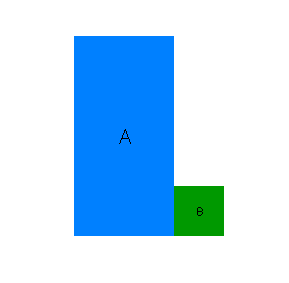
\includegraphics[width=0.2\textwidth]{cp1819t_media/ex2.png}
%
\caption{Caixa simples e caixa composta.\label{fig:L2D}}
\end{figure}

\begin{figure}
\centering
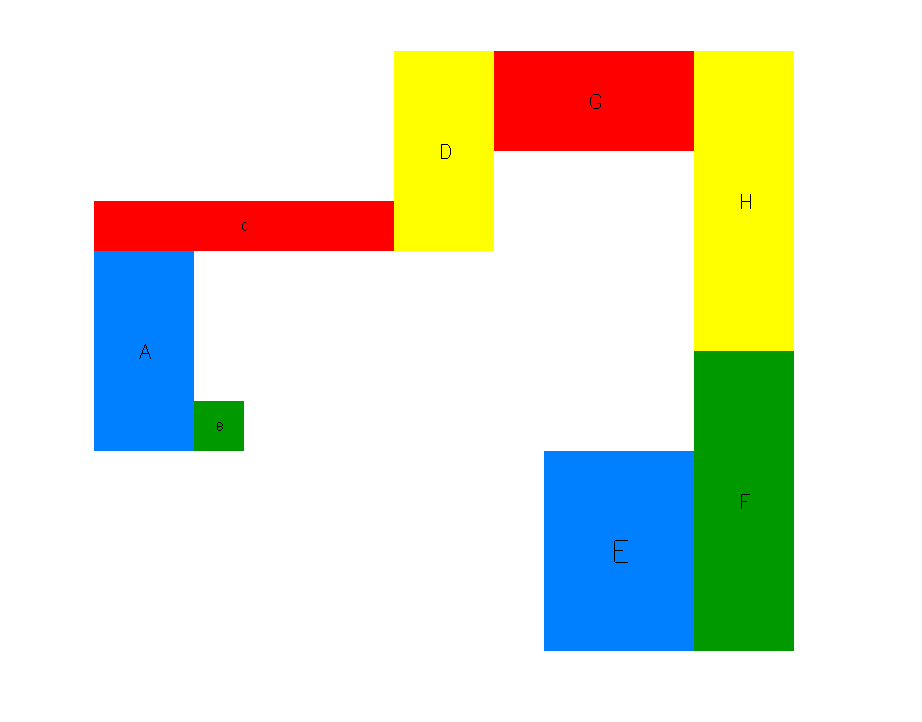
\includegraphics[width=0.6\textwidth]{cp1819t_media/ex.png}
\caption{\uk{Layout} feito de várias caixas coloridas.\label{fig:L2D1}}
\end{figure}

É importante notar que cada ``caixa'' não dispõe informação relativa
ao seu posicionamento final na figura. De facto, é a posição relativa
que deve ocupar face às restantes caixas que irá determinar a sua
posição final. Este é um dos objectivos deste trabalho:
\emph{calcular o posicionamento absoluto de cada uma das caixas por forma a
respeitar as restrições impostas pelas diversas agregações}. Para isso vamos
considerar um tipo de dados que comporta a informação de todas as
caixas devidamente posicionadas (i.e. com a informação adicional da
origem onde a caixa deve ser colocada).

\begin{hscode}\SaveRestoreHook
\column{B}{@{}>{\hspre}l<{\hspost}@{}}%
\column{E}{@{}>{\hspre}l<{\hspost}@{}}%
\>[B]{}\mathbf{type}\;\Conid{Fig}\mathrel{=}[\mskip1.5mu (\Conid{Origem},\Conid{Caixa})\mskip1.5mu]{}\<[E]%
\\
\>[B]{}\mathbf{type}\;\Conid{Origem}\mathrel{=}(\Conid{Float},\Conid{Float}){}\<[E]%
\ColumnHook
\end{hscode}\resethooks
%
A informação mais relevante deste tipo é a referente à lista de
``caixas posicionadas'' (tipo \ensuremath{(\Conid{Origem},\Conid{Caixa})}). Regista-se aí a origem
da caixa que, com a informação da sua altura e comprimento, permite
definir todos os seus pontos (consideramos as caixas sempre paralelas
aos eixos). 

\begin{enumerate}
\item Forneça a definição da função \ensuremath{\Varid{calc\char95 origems}}, que calcula as
coordenadas iniciais das caixas no plano:
\begin{hscode}\SaveRestoreHook
\column{B}{@{}>{\hspre}l<{\hspost}@{}}%
\column{E}{@{}>{\hspre}l<{\hspost}@{}}%
\>[B]{}\Varid{calc\char95 origems}\mathbin{::}(\Conid{L2D},\Conid{Origem})\to \Conid{X}\;(\Conid{Caixa},\Conid{Origem})\;(){}\<[E]%
\ColumnHook
\end{hscode}\resethooks
\item Forneça agora a definição da função \ensuremath{\Varid{agrup\char95 caixas}}, que agrupa
todas as caixas e respectivas origens numa só lista:
\begin{hscode}\SaveRestoreHook
\column{B}{@{}>{\hspre}l<{\hspost}@{}}%
\column{E}{@{}>{\hspre}l<{\hspost}@{}}%
\>[B]{}\Varid{agrup\char95 caixas}\mathbin{::}\Conid{X}\;(\Conid{Caixa},\Conid{Origem})\;()\to \Conid{Fig}{}\<[E]%
\ColumnHook
\end{hscode}\resethooks
\end{enumerate}

Um segundo problema neste projecto é \emph{descobrir como visualizar a
informação gráfica calculada por \ensuremath{\Varid{desenho}}}. A nossa estratégia para
superar o problema baseia-se na biblioteca \gloss{Gloss}, que permite a geração
de gráficos 2D. Para tal disponibiliza-se a função
\begin{hscode}\SaveRestoreHook
\column{B}{@{}>{\hspre}l<{\hspost}@{}}%
\column{20}{@{}>{\hspre}l<{\hspost}@{}}%
\column{E}{@{}>{\hspre}l<{\hspost}@{}}%
\>[B]{}\Varid{crCaixa}\mathbin{::}\Conid{Origem}{}\<[20]%
\>[20]{}\to \Conid{Float}\to \Conid{Float}\to \Conid{String}\to \Conid{\Conid{G}.Color}\to \Conid{\Conid{G}.Picture}{}\<[E]%
\ColumnHook
\end{hscode}\resethooks
que cria um rectângulo com base numa coordenada, um valor para a largura, um valor
para a altura, um texto que irá servir de etiqueta, e a cor pretendida.
Disponibiliza-se também a função
\begin{hscode}\SaveRestoreHook
\column{B}{@{}>{\hspre}l<{\hspost}@{}}%
\column{E}{@{}>{\hspre}l<{\hspost}@{}}%
\>[B]{}\Varid{display}\mathbin{::}\Conid{\Conid{G}.Picture}\to \fun{IO}\;(){}\<[E]%
\ColumnHook
\end{hscode}\resethooks
que dado um valor do tipo \ensuremath{\Varid{\Conid{G}.picture}} abre uma janela com esse valor desenhado. O objectivo
final deste exercício é implementar então uma função 
\begin{hscode}\SaveRestoreHook
\column{B}{@{}>{\hspre}l<{\hspost}@{}}%
\column{E}{@{}>{\hspre}l<{\hspost}@{}}%
\>[B]{}\Varid{mostra\char95 caixas}\mathbin{::}(\Conid{L2D},\Conid{Origem})\to \fun{IO}\;(){}\<[E]%
\ColumnHook
\end{hscode}\resethooks
que dada uma frase da linguagem \ensuremath{\Conid{L2D}} e coordenadas iniciais apresenta
o respectivo desenho no ecrã.
%
\textbf{Sugestão}: 
Use a função \ensuremath{\Varid{\Conid{G}.pictures}} disponibilizada na biblioteca \gloss{Gloss}.

\Problema

Nesta disciplina estudou-se como fazer \pd{programação dinâmica} por cálculo,
recorrendo à lei de recursividade mútua.\footnote{Lei (\ref{eq:fokkinga})
em \cite{Ol18}, página \pageref{eq:fokkinga}.}

Para o caso de funções sobre os números naturais (\ensuremath{\N_0}, com functor \ensuremath{\fun F \;\Conid{X}\mathrel{=}\mathrm{1}\mathbin{+}\Conid{X}}) é fácil derivar-se da lei que foi estudada uma
	\emph{regra de algibeira}
	\label{pg:regra}
que se pode ensinar a programadores que não tenham estudado
\cp{Cálculo de Programas}. Apresenta-se de seguida essa regra, tomando como exemplo o
cálculo do ciclo-\textsf{for} que implementa a função de Fibonacci, recordar
o sistema
\begin{hscode}\SaveRestoreHook
\column{B}{@{}>{\hspre}l<{\hspost}@{}}%
\column{E}{@{}>{\hspre}l<{\hspost}@{}}%
\>[B]{}\Varid{fib}\;\mathrm{0}\mathrel{=}\mathrm{1}{}\<[E]%
\\
\>[B]{}\Varid{fib}\;(\Varid{n}\mathbin{+}\mathrm{1})\mathrel{=}\Varid{f}\;\Varid{n}{}\<[E]%
\\[\blanklineskip]%
\>[B]{}\Varid{f}\;\mathrm{0}\mathrel{=}\mathrm{1}{}\<[E]%
\\
\>[B]{}\Varid{f}\;(\Varid{n}\mathbin{+}\mathrm{1})\mathrel{=}\Varid{fib}\;\Varid{n}\mathbin{+}\Varid{f}\;\Varid{n}{}\<[E]%
\ColumnHook
\end{hscode}\resethooks
Obter-se-á de imediato
\begin{hscode}\SaveRestoreHook
\column{B}{@{}>{\hspre}l<{\hspost}@{}}%
\column{4}{@{}>{\hspre}l<{\hspost}@{}}%
\column{E}{@{}>{\hspre}l<{\hspost}@{}}%
\>[B]{}\Varid{fib'}\mathrel{=}\p1\comp \for{\Varid{loop}}\ {\Varid{init}}\;\mathbf{where}{}\<[E]%
\\
\>[B]{}\hsindent{4}{}\<[4]%
\>[4]{}\Varid{loop}\;(\Varid{fib},\Varid{f})\mathrel{=}(\Varid{f},\Varid{fib}\mathbin{+}\Varid{f}){}\<[E]%
\\
\>[B]{}\hsindent{4}{}\<[4]%
\>[4]{}\Varid{init}\mathrel{=}(\mathrm{1},\mathrm{1}){}\<[E]%
\ColumnHook
\end{hscode}\resethooks
usando as regras seguintes:
\begin{itemize}
\item	O corpo do ciclo \ensuremath{\Varid{loop}} terá tantos argumentos quanto o número de funções mutuamente recursivas.
\item	Para as variáveis escolhem-se os próprios nomes das funções, pela ordem
que se achar conveniente.\footnote{Podem obviamente usar-se outros símbolos, mas numa primeiraleitura
dá jeito usarem-se tais nomes.}
\item	Para os resultados vão-se buscar as expressões respectivas, retirando a variável \ensuremath{\Varid{n}}.
\item	Em \ensuremath{\Varid{init}} coleccionam-se os resultados dos casos de base das funções, pela mesma ordem.
\end{itemize}
Mais um exemplo, envolvendo polinómios no segundo grau a $x^2 + b x + c$ em \ensuremath{\N_0}.
Seguindo o método estudado nas aulas\footnote{Secção 3.17 de \cite{Ol18}.},
de $f\ x = a x^2 + b x + c$ derivam-se duas funções mutuamente recursivas:
\begin{hscode}\SaveRestoreHook
\column{B}{@{}>{\hspre}l<{\hspost}@{}}%
\column{E}{@{}>{\hspre}l<{\hspost}@{}}%
\>[B]{}\Varid{f}\;\mathrm{0}\mathrel{=}\Varid{c}{}\<[E]%
\\
\>[B]{}\Varid{f}\;(\Varid{n}\mathbin{+}\mathrm{1})\mathrel{=}\Varid{f}\;\Varid{n}\mathbin{+}\Varid{k}\;\Varid{n}{}\<[E]%
\\[\blanklineskip]%
\>[B]{}\Varid{k}\;\mathrm{0}\mathrel{=}\Varid{a}\mathbin{+}\Varid{b}{}\<[E]%
\\
\>[B]{}\Varid{k}\;(\Varid{n}\mathbin{+}\mathrm{1})\mathrel{=}\Varid{k}\;\Varid{n}\mathbin{+}\mathrm{2}\;\Varid{a}{}\<[E]%
\ColumnHook
\end{hscode}\resethooks
Seguindo a regra acima, calcula-se de imediato a seguinte implementação, em Haskell:
\begin{hscode}\SaveRestoreHook
\column{B}{@{}>{\hspre}l<{\hspost}@{}}%
\column{3}{@{}>{\hspre}l<{\hspost}@{}}%
\column{E}{@{}>{\hspre}l<{\hspost}@{}}%
\>[B]{}\Varid{f'}\;\Varid{a}\;\Varid{b}\;\Varid{c}\mathrel{=}\p1\comp \for{\Varid{loop}}\ {\Varid{init}}\;\mathbf{where}{}\<[E]%
\\
\>[B]{}\hsindent{3}{}\<[3]%
\>[3]{}\Varid{loop}\;(\Varid{f},\Varid{k})\mathrel{=}(\Varid{f}\mathbin{+}\Varid{k},\Varid{k}\mathbin{+}\mathrm{2}\mathbin{*}\Varid{a}){}\<[E]%
\\
\>[B]{}\hsindent{3}{}\<[3]%
\>[3]{}\Varid{init}\mathrel{=}(\Varid{c},\Varid{a}\mathbin{+}\Varid{b}){}\<[E]%
\ColumnHook
\end{hscode}\resethooks

Qual é o assunto desta questão, então? Considerem fórmula que dá a série de Taylor da
função coseno:
\begin{eqnarray*}
	cos\ x = \sum_{i=0}^\infty \frac{(-1)^i}{(2i)!} x^{2i}
\end{eqnarray*}
Pretende-se o ciclo-\textsf{for} que implementa a função 
\ensuremath{\Varid{cos'}\;\Varid{x}\;\Varid{n}} que dá o valor dessa série tomando \ensuremath{\Varid{i}} até \ensuremath{\Varid{n}} inclusivé:
\begin{hscode}\SaveRestoreHook
\column{B}{@{}>{\hspre}l<{\hspost}@{}}%
\column{E}{@{}>{\hspre}l<{\hspost}@{}}%
\>[B]{}\Varid{cos'}\;\Varid{x}\mathrel{=}\cdots \comp \for{\Varid{loop}}\ {\Varid{init}}\;\mathbf{where}\;\cdots {}\<[E]%
\ColumnHook
\end{hscode}\resethooks
%
\textbf{Sugestão}: Começar por estudar muito bem o processo de cálculo dado
no anexo \ref{sec:recmul} para o problema (semelhante) da função exponencial.

\begin{propriedade}
Testes de que \ensuremath{\Varid{cos'}\;\Varid{x}} calcula bem o coseno de \ensuremath{\pi } e o coseno de \ensuremath{\pi \mathbin{/}\mathrm{2}}:
\begin{hscode}\SaveRestoreHook
\column{B}{@{}>{\hspre}l<{\hspost}@{}}%
\column{E}{@{}>{\hspre}l<{\hspost}@{}}%
\>[B]{}\Varid{prop\char95 cos1}\;\Varid{n}\mathrel{=}\Varid{n}\geq \mathrm{10}\Rightarrow\Varid{abs}\;(\Varid{cos}\;\pi \mathbin{-}\Varid{cos'}\;\pi \;\Varid{n})\mathbin{<}\mathrm{0.001}{}\<[E]%
\\
\>[B]{}\Varid{prop\char95 cos2}\;\Varid{n}\mathrel{=}\Varid{n}\geq \mathrm{10}\Rightarrow\Varid{abs}\;(\Varid{cos}\;(\pi \mathbin{/}\mathrm{2})\mathbin{-}\Varid{cos'}\;(\pi \mathbin{/}\mathrm{2})\;\Varid{n})\mathbin{<}\mathrm{0.001}{}\<[E]%
\ColumnHook
\end{hscode}\resethooks
\end{propriedade}

\paragraph{Valorização} Transliterar \ensuremath{\Varid{cos'}} para a linguagem C; compilar
e testar o código. Conseguia, por intuição apenas, chegar a esta função?

\Problema

Pretende-se nesta questão desenvolver uma biblioteca de funções para
manipular \emph{sistemas de ficheiros} genéricos.
Um sistema de ficheiros será visto como uma associação de \emph{nomes}
a ficheiros ou \emph{directorias}.
Estas últimas serão vistas como sub-sistemas de ficheiros e assim
recursivamente.
Assumindo que \ensuremath{\Varid{a}} é o tipo dos identificadores dos ficheiros e
directorias, e que \ensuremath{\Varid{b}} é o tipo do conteúdo dos ficheiros,
podemos definir um tipo indutivo de dados para representar sistemas de
ficheiros da seguinte forma:
\begin{hscode}\SaveRestoreHook
\column{B}{@{}>{\hspre}l<{\hspost}@{}}%
\column{E}{@{}>{\hspre}l<{\hspost}@{}}%
\>[B]{}\mathbf{data}\;\Conid{FS}\;\Varid{a}\;\Varid{b}\mathrel{=}\Conid{FS}\;[\mskip1.5mu (\Varid{a},\Conid{Node}\;\Varid{a}\;\Varid{b})\mskip1.5mu]\;\mathbf{deriving}\;(\Conid{Eq},\Conid{Show}){}\<[E]%
\\
\>[B]{}\mathbf{data}\;\Conid{Node}\;\Varid{a}\;\Varid{b}\mathrel{=}\Conid{File}\;\Varid{b}\mid \Conid{Dir}\;(\Conid{FS}\;\Varid{a}\;\Varid{b})\;\mathbf{deriving}\;(\Conid{Eq},\Conid{Show}){}\<[E]%
\ColumnHook
\end{hscode}\resethooks
Um caminho (\emph{path}) neste sistema de ficheiros pode ser representado pelo
seguinte tipo de dados:
\begin{hscode}\SaveRestoreHook
\column{B}{@{}>{\hspre}l<{\hspost}@{}}%
\column{E}{@{}>{\hspre}l<{\hspost}@{}}%
\>[B]{}\mathbf{type}\;\Conid{Path}\;\Varid{a}\mathrel{=}[\mskip1.5mu \Varid{a}\mskip1.5mu]{}\<[E]%
\ColumnHook
\end{hscode}\resethooks
Assumindo estes tipos de dados, o seguinte termo
\begin{hscode}\SaveRestoreHook
\column{B}{@{}>{\hspre}l<{\hspost}@{}}%
\column{4}{@{}>{\hspre}c<{\hspost}@{}}%
\column{4E}{@{}l@{}}%
\column{5}{@{}>{\hspre}l<{\hspost}@{}}%
\column{20}{@{}>{\hspre}l<{\hspost}@{}}%
\column{21}{@{}>{\hspre}l<{\hspost}@{}}%
\column{E}{@{}>{\hspre}l<{\hspost}@{}}%
\>[B]{}\Conid{FS}\;[\mskip1.5mu (\text{\tt \char34 f1\char34},\Conid{File}\;\text{\tt \char34 Ola\char34}),{}\<[E]%
\\
\>[B]{}\hsindent{5}{}\<[5]%
\>[5]{}(\text{\tt \char34 d1\char34},\Conid{Dir}\;(\Conid{FS}\;[\mskip1.5mu (\text{\tt \char34 f2\char34},\Conid{File}\;\text{\tt \char34 Ole\char34}),{}\<[E]%
\\
\>[5]{}\hsindent{16}{}\<[21]%
\>[21]{}(\text{\tt \char34 f3\char34},\Conid{File}\;\text{\tt \char34 Ole\char34}){}\<[E]%
\\
\>[5]{}\hsindent{15}{}\<[20]%
\>[20]{}\mskip1.5mu])){}\<[E]%
\\
\>[B]{}\hsindent{4}{}\<[4]%
\>[4]{}\mskip1.5mu]{}\<[4E]%
\ColumnHook
\end{hscode}\resethooks
representará um sistema de ficheiros em cuja raíz temos um ficheiro chamado
\ensuremath{\Varid{f1}} com conteúdo \ensuremath{\text{\tt \char34 Ola\char34}} e uma directoria chamada \ensuremath{\text{\tt \char34 d1\char34}} constituída por dois
ficheiros, um chamado \ensuremath{\text{\tt \char34 f2\char34}} e outro chamado \ensuremath{\text{\tt \char34 f3\char34}}, ambos com conteúdo \ensuremath{\text{\tt \char34 Ole\char34}}.
%
Neste caso, tanto o tipo dos identificadores como o tipo do conteúdo dos
ficheiros é \ensuremath{\Conid{String}}. No caso geral, o conteúdo de um ficheiro é arbitrário:
pode ser um binário, um texto, uma colecção de dados, etc.

A definição das usuais funções \ensuremath{\Varid{inFS}} e \ensuremath{\Varid{recFS}} para este tipo é a seguinte:
\begin{hscode}\SaveRestoreHook
\column{B}{@{}>{\hspre}l<{\hspost}@{}}%
\column{E}{@{}>{\hspre}l<{\hspost}@{}}%
\>[B]{}\Varid{inFS}\mathrel{=}\Conid{FS}\comp \map \;(\Varid{id}\times\Varid{inNode}){}\<[E]%
\\
\>[B]{}\Varid{inNode}\mathrel{=}\alt{\Conid{File}}{\Conid{Dir}}{}\<[E]%
\\[\blanklineskip]%
\>[B]{}\Varid{recFS}\;\Varid{f}\mathrel{=}\Varid{baseFS}\;\Varid{id}\;\Varid{id}\;\Varid{f}{}\<[E]%
\ColumnHook
\end{hscode}\resethooks
Suponha que se pretende definir como um \ensuremath{\Varid{catamorfismo}} a função que
conta o número de ficheiros existentes num sistema de ficheiros. Uma
possível definição para esta função seria:
\begin{hscode}\SaveRestoreHook
\column{B}{@{}>{\hspre}l<{\hspost}@{}}%
\column{E}{@{}>{\hspre}l<{\hspost}@{}}%
\>[B]{}\Varid{conta}\mathbin{::}\Conid{FS}\;\Varid{a}\;\Varid{b}\to \Conid{Int}{}\<[E]%
\\
\>[B]{}\Varid{conta}\mathrel{=}\Varid{cataFS}\;(\Varid{sum}\comp \map \;(\alt{\underline{\mathrm{1}}}{\Varid{id}}\comp \p2)){}\<[E]%
\ColumnHook
\end{hscode}\resethooks
O que é para fazer:
\begin{enumerate}
\item Definir as funções \ensuremath{\Varid{outFS}}, \ensuremath{\Varid{baseFS}}, \ensuremath{\Varid{cataFS}}, \ensuremath{\Varid{anaFS}} e \ensuremath{\Varid{hyloFS}}.

\item Apresentar, no relatório, o diagrama de \ensuremath{\Varid{cataFS}}.

\item Definir as seguintes funções para manipulação de sistemas de
  ficheiros usando, obrigatoriamente, catamorfismos, anamorfismos ou
  hilomorfismos:

  \begin{enumerate}
  \item Verificação da integridade do sistema de ficheiros (i.e. verificar
    que não existem identificadores repetidos dentro da mesma directoria). \\
    \ensuremath{\Varid{check}\mathbin{::}\Conid{FS}\;\Varid{a}\;\Varid{b}\to \Conid{Bool}}
  \begin{propriedade}
    A integridade de um sistema de ficheiros não depende da ordem em que os    
    últimos são listados na sua directoria:
\begin{hscode}\SaveRestoreHook
\column{B}{@{}>{\hspre}l<{\hspost}@{}}%
\column{E}{@{}>{\hspre}l<{\hspost}@{}}%
\>[B]{}\Varid{prop\char95 check}\mathbin{::}\Conid{FS}\;\Conid{String}\;\Conid{String}\to \Conid{Bool}{}\<[E]%
\\
\>[B]{}\Varid{prop\char95 check}\mathrel{=}\Varid{check}\comp (\Varid{cataFS}\;(\Varid{inFS}\comp \Varid{reverse}))\equiv\Varid{check}{}\<[E]%
\ColumnHook
\end{hscode}\resethooks
  \end{propriedade}  
  \item Recolha do conteúdo de todos os ficheiros num arquivo indexado pelo \emph{path}.\\
    \ensuremath{\Varid{tar}\mathbin{::}\Conid{FS}\;\Varid{a}\;\Varid{b}\to [\mskip1.5mu (\Conid{Path}\;\Varid{a},\Varid{b})\mskip1.5mu]}
  \begin{propriedade}
    O número de ficheiros no sistema deve ser igual ao número de ficheiros
    listados pela função \ensuremath{\Varid{tar}}.
\begin{hscode}\SaveRestoreHook
\column{B}{@{}>{\hspre}l<{\hspost}@{}}%
\column{E}{@{}>{\hspre}l<{\hspost}@{}}%
\>[B]{}\Varid{prop\char95 tar}\mathbin{::}\Conid{FS}\;\Conid{String}\;\Conid{String}\to \Conid{Bool}{}\<[E]%
\\
\>[B]{}\Varid{prop\char95 tar}\mathrel{=}\length \comp \Varid{tar}\equiv\Varid{conta}{}\<[E]%
\ColumnHook
\end{hscode}\resethooks
  \end{propriedade}  
  \item Transformação de um arquivo com o conteúdo dos ficheiros
    indexado pelo \emph{path} num sistema de ficheiros.\\
    \ensuremath{\Varid{untar}\mathbin{::}[\mskip1.5mu (\Conid{Path}\;\Varid{a},\Varid{b})\mskip1.5mu]\to \Conid{FS}\;\Varid{a}\;\Varid{b}} \\
  \textbf{Sugestão}: Use a função \ensuremath{\Varid{joinDupDirs}} para juntar directorias que estejam na mesma
  pasta e que possuam o mesmo identificador.
  \begin{propriedade}
    A composição \ensuremath{\Varid{tar}\comp \Varid{untar}} preserva o número de ficheiros no sistema.
\begin{hscode}\SaveRestoreHook
\column{B}{@{}>{\hspre}l<{\hspost}@{}}%
\column{E}{@{}>{\hspre}l<{\hspost}@{}}%
\>[B]{}\Varid{prop\char95 untar}\mathbin{::}[\mskip1.5mu (\Conid{Path}\;\Conid{String},\Conid{String})\mskip1.5mu]\to \Conid{Property}{}\<[E]%
\\
\>[B]{}\Varid{prop\char95 untar}\mathrel{=}\Varid{validPaths}\Rightarrow((\length \comp \Varid{tar}\comp \Varid{untar})\equiv\length ){}\<[E]%
\\
\>[B]{}\Varid{validPaths}\mathbin{::}[\mskip1.5mu (\Conid{Path}\;\Conid{String},\Conid{String})\mskip1.5mu]\to \Conid{Bool}{}\<[E]%
\\
\>[B]{}\Varid{validPaths}\mathrel{=}(\equiv \mathrm{0})\comp \length \comp (\Varid{filter}\;(\lambda (\Varid{a},\anonymous )\to \length \;\Varid{a}\equiv \mathrm{0})){}\<[E]%
\ColumnHook
\end{hscode}\resethooks
\end{propriedade}  
  \item Localização de todos os \emph{paths} onde existe um
    determinado ficheiro.\\
    \ensuremath{\Varid{find}\mathbin{::}\Varid{a}\to \Conid{FS}\;\Varid{a}\;\Varid{b}\to [\mskip1.5mu \Conid{Path}\;\Varid{a}\mskip1.5mu]}
  \begin{propriedade}
    A composição \ensuremath{\Varid{tar}\comp \Varid{untar}} preserva todos os ficheiros no sistema.
\begin{hscode}\SaveRestoreHook
\column{B}{@{}>{\hspre}l<{\hspost}@{}}%
\column{7}{@{}>{\hspre}l<{\hspost}@{}}%
\column{E}{@{}>{\hspre}l<{\hspost}@{}}%
\>[B]{}\Varid{prop\char95 find}\mathbin{::}\Conid{String}\to \Conid{FS}\;\Conid{String}\;\Conid{String}\to \Conid{Bool}{}\<[E]%
\\
\>[B]{}\Varid{prop\char95 find}\mathrel{=}\Varid{curry}\mathbin{\$}{}\<[E]%
\\
\>[B]{}\hsindent{7}{}\<[7]%
\>[7]{}\length \comp \uncurry{\Varid{find}}\equiv\length \comp \uncurry{\Varid{find}}\comp (\Varid{id}\times(\Varid{untar}\comp \Varid{tar})){}\<[E]%
\ColumnHook
\end{hscode}\resethooks
  \end{propriedade}  
  \item Criação de um novo ficheiro num determinado \emph{path}.\\
    \ensuremath{\Varid{new}\mathbin{::}\Conid{Path}\;\Varid{a}\to \Varid{b}\to \Conid{FS}\;\Varid{a}\;\Varid{b}\to \Conid{FS}\;\Varid{a}\;\Varid{b}}
  \begin{propriedade}
A adição de um ficheiro não existente no sistema não origina ficheiros duplicados.
\begin{hscode}\SaveRestoreHook
\column{B}{@{}>{\hspre}l<{\hspost}@{}}%
\column{7}{@{}>{\hspre}l<{\hspost}@{}}%
\column{47}{@{}>{\hspre}l<{\hspost}@{}}%
\column{E}{@{}>{\hspre}l<{\hspost}@{}}%
\>[B]{}\Varid{prop\char95 new}\mathbin{::}((\Conid{Path}\;\Conid{String},\Conid{String}),\Conid{FS}\;\Conid{String}\;\Conid{String})\to \Conid{Property}{}\<[E]%
\\
\>[B]{}\Varid{prop\char95 new}\mathrel{=}((\Varid{validPath}\wedge\Varid{notDup})\wedge(\Varid{check}\comp \p2))\Rightarrow{}\<[E]%
\\
\>[B]{}\hsindent{7}{}\<[7]%
\>[7]{}(\Varid{checkFiles}\comp \uncurry{\uncurry{\Varid{new}}})\;{}\<[47]%
\>[47]{}\mathbf{where}{}\<[E]%
\\
\>[B]{}\hsindent{7}{}\<[7]%
\>[7]{}\Varid{validPath}\mathrel{=}(\not\equiv \mathrm{0})\comp \length \comp \p1\comp \p1{}\<[E]%
\\
\>[B]{}\hsindent{7}{}\<[7]%
\>[7]{}\Varid{notDup}\mathrel{=}\neg \comp \uncurry{\Varid{elem}}\comp (\p1\times((\mathsf{fmap}\;\p1)\comp \Varid{tar})){}\<[E]%
\ColumnHook
\end{hscode}\resethooks
\textbf{Questão}: Supondo-se que no código acima se substitui a propriedade
\ensuremath{\Varid{checkFiles}} pela propriedade mais fraca \ensuremath{\Varid{check}}, será que a propriedade
\ensuremath{\Varid{prop\char95 new}} ainda é válida? Justifique a sua resposta. 
\end{propriedade}
 
\begin{propriedade}
	A listagem de ficheiros logo após uma adição nunca poderá ser menor que a listagem
	de ficheiros antes dessa mesma adição.
\begin{hscode}\SaveRestoreHook
\column{B}{@{}>{\hspre}l<{\hspost}@{}}%
\column{7}{@{}>{\hspre}l<{\hspost}@{}}%
\column{E}{@{}>{\hspre}l<{\hspost}@{}}%
\>[B]{}\Varid{prop\char95 new2}\mathbin{::}((\Conid{Path}\;\Conid{String},\Conid{String}),\Conid{FS}\;\Conid{String}\;\Conid{String})\to \Conid{Property}{}\<[E]%
\\
\>[B]{}\Varid{prop\char95 new2}\mathrel{=}\Varid{validPath}\Rightarrow((\length \comp \Varid{tar}\comp \p2)\leq(\length \comp \Varid{tar}\comp \uncurry{\uncurry{\Varid{new}}}))\;\mathbf{where}{}\<[E]%
\\
\>[B]{}\hsindent{7}{}\<[7]%
\>[7]{}\Varid{validPath}\mathrel{=}(\not\equiv \mathrm{0})\comp \length \comp \p1\comp \p1{}\<[E]%
\ColumnHook
\end{hscode}\resethooks
  \end{propriedade}  
  \item Duplicação de um ficheiro.\\
    \ensuremath{\Varid{cp}\mathbin{::}\Conid{Path}\;\Varid{a}\to \Conid{Path}\;\Varid{a}\to \Conid{FS}\;\Varid{a}\;\Varid{b}\to \Conid{FS}\;\Varid{a}\;\Varid{b}}
  \begin{propriedade}
    A listagem de ficheiros com um dado nome não diminui após uma duplicação.
\begin{hscode}\SaveRestoreHook
\column{B}{@{}>{\hspre}l<{\hspost}@{}}%
\column{13}{@{}>{\hspre}l<{\hspost}@{}}%
\column{42}{@{}>{\hspre}l<{\hspost}@{}}%
\column{E}{@{}>{\hspre}l<{\hspost}@{}}%
\>[B]{}\Varid{prop\char95 cp}\mathbin{::}((\Conid{Path}\;\Conid{String},\Conid{Path}\;\Conid{String}),{}\<[42]%
\>[42]{}\Conid{FS}\;\Conid{String}\;\Conid{String})\to \Conid{Bool}{}\<[E]%
\\
\>[B]{}\Varid{prop\char95 cp}\mathrel{=}{}\<[13]%
\>[13]{}\length \comp \Varid{tar}\comp \p2\leq\length \comp \Varid{tar}\comp \uncurry{\uncurry{\Varid{cp}}}{}\<[E]%
\ColumnHook
\end{hscode}\resethooks
  \end{propriedade}  
  \item Eliminação de um ficheiro.\\
    \ensuremath{\Varid{rm}\mathbin{::}\Conid{Path}\;\Varid{a}\to \Conid{FS}\;\Varid{a}\;\Varid{b}\to \Conid{FS}\;\Varid{a}\;\Varid{b}}

  \textbf{Sugestão}: Construir um anamorfismo \ensuremath{\Varid{nav}\mathbin{::}(\Conid{Path}\;\Varid{a},\Conid{FS}\;\Varid{a}\;\Varid{b})\to \Conid{FS}\;\Varid{a}\;\Varid{b}}
  que navegue por um sistema de ficheiros tendo como base o \ensuremath{\Varid{path}} dado como argumento.
    \begin{propriedade}
    Remover duas vezes o mesmo ficheiro tem o mesmo efeito que o remover apenas uma vez.
\begin{hscode}\SaveRestoreHook
\column{B}{@{}>{\hspre}l<{\hspost}@{}}%
\column{E}{@{}>{\hspre}l<{\hspost}@{}}%
\>[B]{}\Varid{prop\char95 rm}\mathbin{::}(\Conid{Path}\;\Conid{String},\Conid{FS}\;\Conid{String}\;\Conid{String})\to \Conid{Bool}{}\<[E]%
\\
\>[B]{}\Varid{prop\char95 rm}\mathrel{=}\uncurry{\Varid{rm}}\comp \conj{\p1}{\uncurry{\Varid{rm}}}\equiv\uncurry{\Varid{rm}}{}\<[E]%
\ColumnHook
\end{hscode}\resethooks
\end{propriedade}
\begin{propriedade}
Adicionar um ficheiro e de seguida remover o mesmo não origina novos ficheiros no sistema.
\begin{hscode}\SaveRestoreHook
\column{B}{@{}>{\hspre}l<{\hspost}@{}}%
\column{10}{@{}>{\hspre}l<{\hspost}@{}}%
\column{23}{@{}>{\hspre}l<{\hspost}@{}}%
\column{E}{@{}>{\hspre}l<{\hspost}@{}}%
\>[B]{}\Varid{prop\char95 rm2}\mathbin{::}((\Conid{Path}\;\Conid{String},\Conid{String}),\Conid{FS}\;\Conid{String}\;\Conid{String})\to \Conid{Property}{}\<[E]%
\\
\>[B]{}\Varid{prop\char95 rm2}\mathrel{=}\Varid{validPath}{}\<[23]%
\>[23]{}\Rightarrow((\length \comp \Varid{tar}\comp \uncurry{\Varid{rm}}\comp \conj{\p1\comp \p1}{\uncurry{\uncurry{\Varid{new}}}}){}\<[E]%
\\
\>[B]{}\hsindent{10}{}\<[10]%
\>[10]{}\leq(\length \comp \Varid{tar}\comp \p2))\;\mathbf{where}{}\<[E]%
\\
\>[B]{}\hsindent{10}{}\<[10]%
\>[10]{}\Varid{validPath}\mathrel{=}(\not\equiv \mathrm{0})\comp \length \comp \p1\comp \p1{}\<[E]%
\ColumnHook
\end{hscode}\resethooks
\end{propriedade}  
  \end{enumerate}
\end{enumerate}

\paragraph{Valorização} 

Definir uma função para visualizar em \graphviz{Graphviz}
a estrutura de um sistema de ficheiros. A Figura~\ref{ex_prob1}, por exemplo,
apresenta a estrutura de um sistema com precisamente dois ficheiros dentro
de uma directoria chamada \ensuremath{\text{\tt \char34 d1\char34}}. 

Para realizar este exercício será necessário apenas  escrever o anamorfismo
\begin{quote}
\ensuremath{\Varid{cFS2Exp}\mathbin{::}(\Varid{a},\Conid{FS}\;\Varid{a}\;\Varid{b})\to (\Conid{Exp}\;()\;\Varid{a})} 
\end{quote}
que converte a estrutura de um sistema de ficheiros numa árvore de expressões
descrita em \href{http://wiki.di.uminho.pt/twiki/pub/Education/CP/MaterialPedagogico/Exp.hs}{Exp.hs}.
A função \ensuremath{\Varid{dotFS}} depois tratará de passar a estrutura do sistema de ficheiros para o visualizador.
\begin{figure}
\centering
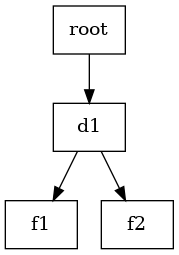
\includegraphics[scale=0.5]{cp1819t_media/fs.png}
\caption{Exemplo de um sistema de ficheiros visualizado em \graphviz{Graphviz}.}
\label{ex_prob1}
\end{figure}

%----------------- Programa, bibliotecas e código auxiliar --------------------%

\newpage

\part*{Anexos}

\appendix

\section{Como exprimir cálculos e diagramas em LaTeX/lhs2tex}
Estudar o texto fonte deste trabalho para obter o efeito:\footnote{Exemplos tirados de \cite{Ol18}.} 
\begin{eqnarray*}
\start
	\ensuremath{\Varid{id}\mathrel{=}\conj{\Varid{f}}{\Varid{g}}}
%
\just\equiv{ universal property }
%
        \ensuremath{\begin{lcbr}\p1\comp \Varid{id}\mathrel{=}\Varid{f}\\\p2\comp \Varid{id}\mathrel{=}\Varid{g}\end{lcbr}}
%
\just\equiv{ identity }
%
        \ensuremath{\begin{lcbr}\p1\mathrel{=}\Varid{f}\\\p2\mathrel{=}\Varid{g}\end{lcbr}}
\qed
\end{eqnarray*}

Os diagramas podem ser produzidos recorrendo à \emph{package} \LaTeX\ 
\href{https://ctan.org/pkg/xymatrix}{xymatrix}, por exemplo: 
\begin{eqnarray*}
\xymatrix@C=2cm{
    \ensuremath{\N_0}
           \ar[d]_-{\ensuremath{\cata{\Varid{g}}}}
&
    \ensuremath{\mathrm{1}\mathbin{+}\N_0}
           \ar[d]^{\ensuremath{\Varid{id}\mathbin{+}\cata{\Varid{g}}}}
           \ar[l]_-{\ensuremath{\mathsf{in}}}
\\
     \ensuremath{\Conid{B}}
&
     \ensuremath{\mathrm{1}\mathbin{+}\Conid{B}}
           \ar[l]^-{\ensuremath{\Varid{g}}}
}
\end{eqnarray*}

\section{Programação dinâmica por recursividade múltipla}\label{sec:recmul}
Neste anexo dão-se os detalhes da resolução do Exercício \ref{ex:exp} dos apontamentos da
disciplina\footnote{Cf.\ \cite{Ol18}, página \pageref{ex:exp}.},
onde se pretende implementar um ciclo que implemente
o cálculo da aproximação até \ensuremath{\Varid{i}\mathrel{=}\Varid{n}} da função exponencial $exp\ x = e^x$
via série de Taylor:
\begin{eqnarray}
	exp\ x 
& = &
	\sum_{i=0}^{\infty} \frac {x^i} {i!}
\end{eqnarray}
Seja $e\ x\ n = \sum_{i=0}^{n} \frac {x^i} {i!}$ a função que dá essa aproximação.
É fácil de ver que \ensuremath{\Varid{e}\;\Varid{x}\;\mathrm{0}\mathrel{=}\mathrm{1}} e que $\ensuremath{\Varid{e}\;\Varid{x}\;(\Varid{n}\mathbin{+}\mathrm{1})} = \ensuremath{\Varid{e}\;\Varid{x}\;\Varid{n}} + \frac {x^{n+1}} {(n+1)!}$.
Se definirmos $\ensuremath{\Varid{h}\;\Varid{x}\;\Varid{n}} = \frac {x^{n+1}} {(n+1)!}$ teremos \ensuremath{\Varid{e}\;\Varid{x}} e \ensuremath{\Varid{h}\;\Varid{x}} em recursividade
mútua. Se repetirmos o processo para \ensuremath{\Varid{h}\;\Varid{x}\;\Varid{n}} etc obteremos no total três funções nessa mesma
situação:
\begin{hscode}\SaveRestoreHook
\column{B}{@{}>{\hspre}l<{\hspost}@{}}%
\column{E}{@{}>{\hspre}l<{\hspost}@{}}%
\>[B]{}\Varid{e}\;\Varid{x}\;\mathrm{0}\mathrel{=}\mathrm{1}{}\<[E]%
\\
\>[B]{}\Varid{e}\;\Varid{x}\;(\Varid{n}\mathbin{+}\mathrm{1})\mathrel{=}\Varid{h}\;\Varid{x}\;\Varid{n}\mathbin{+}\Varid{e}\;\Varid{x}\;\Varid{n}{}\<[E]%
\\[\blanklineskip]%
\>[B]{}\Varid{h}\;\Varid{x}\;\mathrm{0}\mathrel{=}\Varid{x}{}\<[E]%
\\
\>[B]{}\Varid{h}\;\Varid{x}\;(\Varid{n}\mathbin{+}\mathrm{1})\mathrel{=}\Varid{x}\mathbin{/}(\Varid{s}\;\Varid{n})\mathbin{*}\Varid{h}\;\Varid{x}\;\Varid{n}{}\<[E]%
\\[\blanklineskip]%
\>[B]{}\Varid{s}\;\mathrm{0}\mathrel{=}\mathrm{2}{}\<[E]%
\\
\>[B]{}\Varid{s}\;(\Varid{n}\mathbin{+}\mathrm{1})\mathrel{=}\mathrm{1}\mathbin{+}\Varid{s}\;\Varid{n}{}\<[E]%
\ColumnHook
\end{hscode}\resethooks
Segundo a \emph{regra de algibeira} descrita na página \ref{pg:regra} deste enunciado,
ter-se-á, de imediato:
\begin{hscode}\SaveRestoreHook
\column{B}{@{}>{\hspre}l<{\hspost}@{}}%
\column{6}{@{}>{\hspre}l<{\hspost}@{}}%
\column{E}{@{}>{\hspre}l<{\hspost}@{}}%
\>[B]{}\Varid{e'}\;\Varid{x}\mathrel{=}\Varid{prj}\comp \for{\Varid{loop}}\ {\Varid{init}}\;\mathbf{where}{}\<[E]%
\\
\>[B]{}\hsindent{6}{}\<[6]%
\>[6]{}\Varid{init}\mathrel{=}(\mathrm{1},\Varid{x},\mathrm{2}){}\<[E]%
\\
\>[B]{}\hsindent{6}{}\<[6]%
\>[6]{}\Varid{loop}\;(\Varid{e},\Varid{h},\Varid{s})\mathrel{=}(\Varid{h}\mathbin{+}\Varid{e},\Varid{x}\mathbin{/}\Varid{s}\mathbin{*}\Varid{h},\mathrm{1}\mathbin{+}\Varid{s}){}\<[E]%
\\
\>[B]{}\hsindent{6}{}\<[6]%
\>[6]{}\Varid{prj}\;(\Varid{e},\Varid{h},\Varid{s})\mathrel{=}\Varid{e}{}\<[E]%
\ColumnHook
\end{hscode}\resethooks

\section{Código fornecido}\label{sec:codigo}

\subsection*{Problema 1}
Tipos:
\begin{hscode}\SaveRestoreHook
\column{B}{@{}>{\hspre}l<{\hspost}@{}}%
\column{16}{@{}>{\hspre}l<{\hspost}@{}}%
\column{36}{@{}>{\hspre}l<{\hspost}@{}}%
\column{46}{@{}>{\hspre}l<{\hspost}@{}}%
\column{E}{@{}>{\hspre}l<{\hspost}@{}}%
\>[B]{}\mathbf{data}\;\Conid{Expr}\mathrel{=}\Conid{Num}\;\Conid{Int}{}\<[E]%
\\
\>[B]{}\hsindent{16}{}\<[16]%
\>[16]{}\mid \Conid{Bop}\;\Conid{Expr}\;\Conid{Op}\;\Conid{Expr}\;{}\<[36]%
\>[36]{}\mathbf{deriving}\;{}\<[46]%
\>[46]{}(\Conid{Eq},\Conid{Show}){}\<[E]%
\\[\blanklineskip]%
\>[B]{}\mathbf{data}\;\Conid{Op}\mathrel{=}\Conid{Op}\;\Conid{String}\;\mathbf{deriving}\;(\Conid{Eq},\Conid{Show}){}\<[E]%
\\[\blanklineskip]%
\>[B]{}\mathbf{type}\;\Conid{Codigo}\mathrel{=}[\mskip1.5mu \Conid{String}\mskip1.5mu]{}\<[E]%
\ColumnHook
\end{hscode}\resethooks
Functor de base:
\begin{hscode}\SaveRestoreHook
\column{B}{@{}>{\hspre}l<{\hspost}@{}}%
\column{E}{@{}>{\hspre}l<{\hspost}@{}}%
\>[B]{}\Varid{baseExpr}\;\Varid{f}\;\Varid{g}\mathrel{=}\Varid{id}+(\Varid{f}\times(\Varid{g}\times\Varid{g})){}\<[E]%
\ColumnHook
\end{hscode}\resethooks
Instâncias:
\begin{hscode}\SaveRestoreHook
\column{B}{@{}>{\hspre}l<{\hspost}@{}}%
\column{4}{@{}>{\hspre}l<{\hspost}@{}}%
\column{E}{@{}>{\hspre}l<{\hspost}@{}}%
\>[B]{}\mathbf{instance}\;\Conid{Read}\;\Conid{Expr}\;\mathbf{where}{}\<[E]%
\\
\>[B]{}\hsindent{4}{}\<[4]%
\>[4]{}\Varid{readsPrec}\;\anonymous \mathrel{=}\Varid{readExp}{}\<[E]%
\ColumnHook
\end{hscode}\resethooks
Read para Exp's:
\begin{hscode}\SaveRestoreHook
\column{B}{@{}>{\hspre}l<{\hspost}@{}}%
\column{10}{@{}>{\hspre}l<{\hspost}@{}}%
\column{11}{@{}>{\hspre}l<{\hspost}@{}}%
\column{18}{@{}>{\hspre}l<{\hspost}@{}}%
\column{20}{@{}>{\hspre}l<{\hspost}@{}}%
\column{21}{@{}>{\hspre}l<{\hspost}@{}}%
\column{E}{@{}>{\hspre}l<{\hspost}@{}}%
\>[B]{}\Varid{readOp}\mathbin{::}\Conid{String}\to [\mskip1.5mu (\Conid{Op},\Conid{String})\mskip1.5mu]{}\<[E]%
\\
\>[B]{}\Varid{readOp}\;\Varid{input}\mathrel{=}\mathbf{do}{}\<[E]%
\\
\>[B]{}\hsindent{18}{}\<[18]%
\>[18]{}(\Varid{x},\Varid{y})\leftarrow \Varid{lex}\;\Varid{input}{}\<[E]%
\\
\>[B]{}\hsindent{18}{}\<[18]%
\>[18]{}\Varid{return}\;((\Conid{Op}\;\Varid{x}),\Varid{y}){}\<[E]%
\\[\blanklineskip]%
\>[B]{}\Varid{readNum}\mathbin{::}\Conid{ReadS}\;\Conid{Expr}{}\<[E]%
\\
\>[B]{}\Varid{readNum}{}\<[10]%
\>[10]{}\mathrel{=}(\map \;(\lambda (\Varid{x},\Varid{y})\to ((\Conid{Num}\;\Varid{x}),\Varid{y})))\comp \Varid{reads}{}\<[E]%
\\[\blanklineskip]%
\>[B]{}\Varid{readBinOp}\mathbin{::}\Conid{ReadS}\;\Conid{Expr}{}\<[E]%
\\
\>[B]{}\Varid{readBinOp}\mathrel{=}(\map \;(\lambda ((\Varid{x},(\Varid{y},\Varid{z})),\Varid{t})\to ((\Conid{Bop}\;\Varid{x}\;\Varid{y}\;\Varid{z}),\Varid{t})))\comp {}\<[E]%
\\
\>[B]{}\hsindent{20}{}\<[20]%
\>[20]{}((\Varid{readNum}\mathbin{`\Varid{ou}`}(\Varid{pcurvos}\;\Varid{readExp})){}\<[E]%
\\
\>[20]{}\hsindent{1}{}\<[21]%
\>[21]{}\mathbin{`\Varid{depois}`}(\Varid{readOp}\mathbin{`\Varid{depois}`}\Varid{readExp})){}\<[E]%
\\[\blanklineskip]%
\>[B]{}\Varid{readExp}\mathbin{::}\Conid{ReadS}\;\Conid{Expr}{}\<[E]%
\\
\>[B]{}\Varid{readExp}\mathrel{=}\Varid{readBinOp}\mathbin{`\Varid{ou}`}({}\<[E]%
\\
\>[B]{}\hsindent{11}{}\<[11]%
\>[11]{}\Varid{readNum}\mathbin{`\Varid{ou}`}({}\<[E]%
\\
\>[B]{}\hsindent{11}{}\<[11]%
\>[11]{}\Varid{pcurvos}\;\Varid{readExp})){}\<[E]%
\ColumnHook
\end{hscode}\resethooks
Combinadores:
\begin{hscode}\SaveRestoreHook
\column{B}{@{}>{\hspre}l<{\hspost}@{}}%
\column{3}{@{}>{\hspre}l<{\hspost}@{}}%
\column{5}{@{}>{\hspre}l<{\hspost}@{}}%
\column{7}{@{}>{\hspre}l<{\hspost}@{}}%
\column{10}{@{}>{\hspre}l<{\hspost}@{}}%
\column{16}{@{}>{\hspre}l<{\hspost}@{}}%
\column{22}{@{}>{\hspre}l<{\hspost}@{}}%
\column{25}{@{}>{\hspre}l<{\hspost}@{}}%
\column{36}{@{}>{\hspre}l<{\hspost}@{}}%
\column{42}{@{}>{\hspre}l<{\hspost}@{}}%
\column{53}{@{}>{\hspre}l<{\hspost}@{}}%
\column{E}{@{}>{\hspre}l<{\hspost}@{}}%
\>[B]{}\Varid{depois}\mathbin{::}(\Conid{ReadS}\;\Varid{a})\to (\Conid{ReadS}\;\Varid{b})\to \Conid{ReadS}\;(\Varid{a},\Varid{b}){}\<[E]%
\\
\>[B]{}\Varid{depois}\;\anonymous \;\anonymous \;[\mskip1.5mu \mskip1.5mu]\mathrel{=}[\mskip1.5mu \mskip1.5mu]{}\<[E]%
\\
\>[B]{}\Varid{depois}\;\Varid{r1}\;\Varid{r2}\;\Varid{input}\mathrel{=}[\mskip1.5mu ((\Varid{x},\Varid{y}),i_2)\mid (\Varid{x},i_1)\leftarrow \Varid{r1}\;\Varid{input},{}\<[E]%
\\
\>[B]{}\hsindent{36}{}\<[36]%
\>[36]{}(\Varid{y},i_2)\leftarrow \Varid{r2}\;i_1\mskip1.5mu]{}\<[E]%
\\[\blanklineskip]%
\>[B]{}\Varid{readSeq}\mathbin{::}(\Conid{ReadS}\;\Varid{a})\to \Conid{ReadS}\;[\mskip1.5mu \Varid{a}\mskip1.5mu]{}\<[E]%
\\
\>[B]{}\Varid{readSeq}\;\Varid{r}\;\Varid{input}{}\<[E]%
\\
\>[B]{}\hsindent{3}{}\<[3]%
\>[3]{}\mathrel{=}\mathbf{case}\;(\Varid{r}\;\Varid{input})\;\mathbf{of}{}\<[E]%
\\
\>[3]{}\hsindent{2}{}\<[5]%
\>[5]{}[\mskip1.5mu \mskip1.5mu]\to [\mskip1.5mu ([\mskip1.5mu \mskip1.5mu],\Varid{input})\mskip1.5mu]{}\<[E]%
\\
\>[3]{}\hsindent{2}{}\<[5]%
\>[5]{}\Varid{l}\to \Varid{concat}\;(\map \;\Varid{continua}\;\Varid{l}){}\<[E]%
\\
\>[5]{}\hsindent{5}{}\<[10]%
\>[10]{}\mathbf{where}\;\Varid{continua}\;(\Varid{a},\Varid{i})\mathrel{=}\map \;(\Varid{c}\;\Varid{a})\;(\Varid{readSeq}\;\Varid{r}\;\Varid{i}){}\<[E]%
\\
\>[10]{}\hsindent{6}{}\<[16]%
\>[16]{}\Varid{c}\;\Varid{x}\;(\Varid{xs},\Varid{i})\mathrel{=}((\Varid{x}\mathbin{:}\Varid{xs}),\Varid{i}){}\<[E]%
\\[\blanklineskip]%
\>[B]{}\Varid{ou}\mathbin{::}(\Conid{ReadS}\;\Varid{a})\to (\Conid{ReadS}\;\Varid{a})\to \Conid{ReadS}\;\Varid{a}{}\<[E]%
\\
\>[B]{}\Varid{ou}\;\Varid{r1}\;\Varid{r2}\;\Varid{input}\mathrel{=}(\Varid{r1}\;\Varid{input})\plus (\Varid{r2}\;\Varid{input}){}\<[E]%
\\[\blanklineskip]%
\>[B]{}\Varid{senao}\mathbin{::}(\Conid{ReadS}\;\Varid{a})\to (\Conid{ReadS}\;\Varid{a})\to \Conid{ReadS}\;\Varid{a}{}\<[E]%
\\
\>[B]{}\Varid{senao}\;\Varid{r1}\;\Varid{r2}\;\Varid{input}\mathrel{=}\mathbf{case}\;(\Varid{r1}\;\Varid{input})\;\mathbf{of}{}\<[E]%
\\
\>[B]{}\hsindent{22}{}\<[22]%
\>[22]{}[\mskip1.5mu \mskip1.5mu]\to \Varid{r2}\;\Varid{input}{}\<[E]%
\\
\>[B]{}\hsindent{22}{}\<[22]%
\>[22]{}\Varid{l}{}\<[25]%
\>[25]{}\to \Varid{l}{}\<[E]%
\\[\blanklineskip]%
\>[B]{}\Varid{readConst}\mathbin{::}\Conid{String}\to \Conid{ReadS}\;\Conid{String}{}\<[E]%
\\
\>[B]{}\Varid{readConst}\;\Varid{c}\mathrel{=}(\Varid{filter}\;((\equiv \Varid{c})\comp \p1))\comp \Varid{lex}{}\<[E]%
\\[\blanklineskip]%
\>[B]{}\Varid{pcurvos}\mathrel{=}\Varid{parentesis}\;\text{\tt '('}\;\text{\tt ')'}{}\<[E]%
\\
\>[B]{}\Varid{prectos}\mathrel{=}\Varid{parentesis}\;\text{\tt '['}\;\text{\tt ']'}{}\<[E]%
\\
\>[B]{}\Varid{chavetas}\mathrel{=}\Varid{parentesis}\;\text{\tt '\char123 '}\;\text{\tt '\char125 '}{}\<[E]%
\\[\blanklineskip]%
\>[B]{}\Varid{parentesis}\mathbin{::}\Conid{Char}\to \Conid{Char}\to (\Conid{ReadS}\;\Varid{a})\to \Conid{ReadS}\;\Varid{a}{}\<[E]%
\\
\>[B]{}\Varid{parentesis}\;\anonymous \;\anonymous \;\anonymous \;[\mskip1.5mu \mskip1.5mu]\mathrel{=}[\mskip1.5mu \mskip1.5mu]{}\<[E]%
\\
\>[B]{}\Varid{parentesis}\;\Varid{ap}\;\Varid{pa}\;\Varid{r}\;\Varid{input}{}\<[E]%
\\
\>[B]{}\hsindent{3}{}\<[3]%
\>[3]{}\mathrel{=}\mathbf{do}{}\<[E]%
\\
\>[3]{}\hsindent{4}{}\<[7]%
\>[7]{}((\anonymous ,(\Varid{x},\anonymous )),\Varid{c})\leftarrow ((\Varid{readConst}\;[\mskip1.5mu \Varid{ap}\mskip1.5mu])\mathbin{`\Varid{depois}`}({}\<[E]%
\\
\>[7]{}\hsindent{18}{}\<[25]%
\>[25]{}\Varid{r}{}\<[42]%
\>[42]{}\mathbin{`\Varid{depois}`}({}\<[E]%
\\
\>[7]{}\hsindent{18}{}\<[25]%
\>[25]{}\Varid{readConst}\;[\mskip1.5mu \Varid{pa}\mskip1.5mu])))\;{}\<[53]%
\>[53]{}\Varid{input}{}\<[E]%
\\
\>[3]{}\hsindent{4}{}\<[7]%
\>[7]{}\Varid{return}\;(\Varid{x},\Varid{c}){}\<[E]%
\ColumnHook
\end{hscode}\resethooks

\subsection*{Problema 2}
Tipos:
\begin{hscode}\SaveRestoreHook
\column{B}{@{}>{\hspre}l<{\hspost}@{}}%
\column{E}{@{}>{\hspre}l<{\hspost}@{}}%
\>[B]{}\mathbf{type}\;\Conid{Fig}\mathrel{=}[\mskip1.5mu (\Conid{Origem},\Conid{Caixa})\mskip1.5mu]{}\<[E]%
\\
\>[B]{}\mathbf{type}\;\Conid{Origem}\mathrel{=}(\Conid{Float},\Conid{Float}){}\<[E]%
\ColumnHook
\end{hscode}\resethooks
``Helpers":
\begin{hscode}\SaveRestoreHook
\column{B}{@{}>{\hspre}l<{\hspost}@{}}%
\column{E}{@{}>{\hspre}l<{\hspost}@{}}%
\>[B]{}\Varid{col\char95 blue}\mathrel{=}\Varid{\Conid{G}.azure}{}\<[E]%
\\
\>[B]{}\Varid{col\char95 green}\mathrel{=}\Varid{darkgreen}{}\<[E]%
\\[\blanklineskip]%
\>[B]{}\Varid{darkgreen}\mathrel{=}\Varid{\Conid{G}.dark}\;(\Varid{\Conid{G}.dark}\;\Varid{\Conid{G}.green}){}\<[E]%
\ColumnHook
\end{hscode}\resethooks
Exemplos:
\begin{hscode}\SaveRestoreHook
\column{B}{@{}>{\hspre}l<{\hspost}@{}}%
\column{11}{@{}>{\hspre}l<{\hspost}@{}}%
\column{14}{@{}>{\hspre}l<{\hspost}@{}}%
\column{E}{@{}>{\hspre}l<{\hspost}@{}}%
\>[B]{}\Varid{ex1Caixas}\mathrel{=}\Varid{\Conid{G}.display}\;(\Conid{\Conid{G}.InWindow}\;\text{\tt \char34 Problema~4\char34}\;(\mathrm{400},\mathrm{400})\;(\mathrm{40},\mathrm{40}))\;\Varid{\Conid{G}.white}\mathbin{\$}{}\<[E]%
\\
\>[B]{}\hsindent{11}{}\<[11]%
\>[11]{}\Varid{crCaixa}\;(\mathrm{0},\mathrm{0})\;\mathrm{200}\;\mathrm{200}\;\text{\tt \char34 Caixa~azul\char34}\;\Varid{col\char95 blue}{}\<[E]%
\\[\blanklineskip]%
\>[B]{}\Varid{ex2Caixas}\mathrel{=}{}\<[14]%
\>[14]{}\Varid{\Conid{G}.display}\;(\Conid{\Conid{G}.InWindow}\;\text{\tt \char34 Problema~4\char34}\;(\mathrm{400},\mathrm{400})\;(\mathrm{40},\mathrm{40}))\;\Varid{\Conid{G}.white}\mathbin{\$}{}\<[E]%
\\
\>[B]{}\hsindent{11}{}\<[11]%
\>[11]{}\Varid{caixasAndOrigin2Pict}\;((\Conid{Comp}\;\Conid{Hb}\;\Varid{bbox}\;\Varid{gbox}),(\mathrm{0.0},\mathrm{0.0}))\;\mathbf{where}{}\<[E]%
\\
\>[B]{}\hsindent{11}{}\<[11]%
\>[11]{}\Varid{bbox}\mathrel{=}\Conid{Unid}\;((\mathrm{100},\mathrm{200}),(\text{\tt \char34 A\char34},\Varid{col\char95 blue})){}\<[E]%
\\
\>[B]{}\hsindent{11}{}\<[11]%
\>[11]{}\Varid{gbox}\mathrel{=}\Conid{Unid}\;((\mathrm{50},\mathrm{50}),(\text{\tt \char34 B\char34},\Varid{col\char95 green})){}\<[E]%
\\[\blanklineskip]%
\>[B]{}\Varid{ex3Caixas}\mathrel{=}\Varid{\Conid{G}.display}\;(\Conid{\Conid{G}.InWindow}\;\text{\tt \char34 Problema~4\char34}\;(\mathrm{400},\mathrm{400})\;(\mathrm{40},\mathrm{40}))\;\Varid{\Conid{G}.white}\;\Varid{mtest}\;\mathbf{where}{}\<[E]%
\\
\>[B]{}\hsindent{11}{}\<[11]%
\>[11]{}\Varid{mtest}\mathrel{=}\Varid{caixasAndOrigin2Pict}\mathbin{\$}(\Conid{Comp}\;\Conid{Hb}\;(\Conid{Comp}\;\Conid{Ve}\;\Varid{bot}\;\Varid{top})\;(\Conid{Comp}\;\Conid{Ve}\;\Varid{gbox2}\;\Varid{ybox2}),(\mathrm{0.0},\mathrm{0.0})){}\<[E]%
\\
\>[B]{}\hsindent{11}{}\<[11]%
\>[11]{}\Varid{bbox1}\mathrel{=}\Conid{Unid}\;((\mathrm{100},\mathrm{200}),(\text{\tt \char34 A\char34},\Varid{col\char95 blue})){}\<[E]%
\\
\>[B]{}\hsindent{11}{}\<[11]%
\>[11]{}\Varid{bbox2}\mathrel{=}\Conid{Unid}\;((\mathrm{150},\mathrm{200}),(\text{\tt \char34 E\char34},\Varid{col\char95 blue})){}\<[E]%
\\
\>[B]{}\hsindent{11}{}\<[11]%
\>[11]{}\Varid{gbox1}\mathrel{=}\Conid{Unid}\;((\mathrm{50},\mathrm{50}),(\text{\tt \char34 B\char34},\Varid{col\char95 green})){}\<[E]%
\\
\>[B]{}\hsindent{11}{}\<[11]%
\>[11]{}\Varid{gbox2}\mathrel{=}\Conid{Unid}\;((\mathrm{100},\mathrm{300}),(\text{\tt \char34 F\char34},\Varid{col\char95 green})){}\<[E]%
\\
\>[B]{}\hsindent{11}{}\<[11]%
\>[11]{}\Varid{rbox1}\mathrel{=}\Conid{Unid}\;((\mathrm{300},\mathrm{50}),(\text{\tt \char34 C\char34},\Varid{\Conid{G}.red})){}\<[E]%
\\
\>[B]{}\hsindent{11}{}\<[11]%
\>[11]{}\Varid{rbox2}\mathrel{=}\Conid{Unid}\;((\mathrm{200},\mathrm{100}),(\text{\tt \char34 G\char34},\Varid{\Conid{G}.red})){}\<[E]%
\\
\>[B]{}\hsindent{11}{}\<[11]%
\>[11]{}\Varid{wbox1}\mathrel{=}\Conid{Unid}\;((\mathrm{450},\mathrm{200}),(\text{\tt \char34 \char34},\Varid{\Conid{G}.white})){}\<[E]%
\\
\>[B]{}\hsindent{11}{}\<[11]%
\>[11]{}\Varid{ybox1}\mathrel{=}\Conid{Unid}\;((\mathrm{100},\mathrm{200}),(\text{\tt \char34 D\char34},\Varid{\Conid{G}.yellow})){}\<[E]%
\\
\>[B]{}\hsindent{11}{}\<[11]%
\>[11]{}\Varid{ybox2}\mathrel{=}\Conid{Unid}\;((\mathrm{100},\mathrm{300}),(\text{\tt \char34 H\char34},\Varid{\Conid{G}.yellow})){}\<[E]%
\\
\>[B]{}\hsindent{11}{}\<[11]%
\>[11]{}\Varid{bot}\mathrel{=}\Conid{Comp}\;\Conid{Hb}\;\Varid{wbox1}\;\Varid{bbox2}{}\<[E]%
\\
\>[B]{}\hsindent{11}{}\<[11]%
\>[11]{}\Varid{top}\mathrel{=}(\Conid{Comp}\;\Conid{Ve}\;(\Conid{Comp}\;\Conid{Hb}\;\Varid{bbox1}\;\Varid{gbox1})\;(\Conid{Comp}\;\Conid{Hb}\;\Varid{rbox1}\;(\Conid{Comp}\;\Conid{H}\;\Varid{ybox1}\;\Varid{rbox2}))){}\<[E]%
\ColumnHook
\end{hscode}\resethooks
A seguinte função cria uma caixa a partir dos seguintes parâmetros: origem,
largura, altura, etiqueta e côr de preenchimento.
\begin{hscode}\SaveRestoreHook
\column{B}{@{}>{\hspre}l<{\hspost}@{}}%
\column{20}{@{}>{\hspre}l<{\hspost}@{}}%
\column{21}{@{}>{\hspre}l<{\hspost}@{}}%
\column{30}{@{}>{\hspre}l<{\hspost}@{}}%
\column{60}{@{}>{\hspre}l<{\hspost}@{}}%
\column{E}{@{}>{\hspre}l<{\hspost}@{}}%
\>[B]{}\Varid{crCaixa}\mathbin{::}\Conid{Origem}{}\<[20]%
\>[20]{}\to \Conid{Float}\to \Conid{Float}\to \Conid{String}\to \Conid{\Conid{G}.Color}\to \Conid{\Conid{G}.Picture}{}\<[E]%
\\
\>[B]{}\Varid{crCaixa}\;(\Varid{x},\Varid{y})\;\Varid{w}\;\Varid{h}\;\Varid{l}\;\Varid{c}\mathrel{=}\Conid{\Conid{G}.Translate}\;(\Varid{x}\mathbin{+}(\Varid{w}\mathbin{/}\mathrm{2}))\;(\Varid{y}\mathbin{+}(\Varid{h}\mathbin{/}\mathrm{2}))\mathbin{\$}{}\<[60]%
\>[60]{}\Varid{\Conid{G}.pictures}\;[\mskip1.5mu \Varid{caixa},\Varid{etiqueta}\mskip1.5mu]\;\mathbf{where}{}\<[E]%
\\
\>[B]{}\hsindent{21}{}\<[21]%
\>[21]{}\Varid{caixa}\mathrel{=}\Varid{\Conid{G}.color}\;\Varid{c}\;(\Varid{\Conid{G}.rectangleSolid}\;\Varid{w}\;\Varid{h}){}\<[E]%
\\
\>[B]{}\hsindent{21}{}\<[21]%
\>[21]{}\Varid{etiqueta}\mathrel{=}\Varid{\Conid{G}.translate}\;\Varid{calc\char95 trans\char95 x}\;\Varid{calc\char95 trans\char95 y}\mathbin{\$}{}\<[E]%
\\
\>[21]{}\hsindent{9}{}\<[30]%
\>[30]{}\Conid{\Conid{G}.Scale}\;\Varid{calc\char95 scale}\;\Varid{calc\char95 scale}\mathbin{\$}\Varid{\Conid{G}.color}\;\Varid{\Conid{G}.black}\mathbin{\$}\Conid{\Conid{G}.Text}\;\Varid{l}{}\<[E]%
\\
\>[B]{}\hsindent{21}{}\<[21]%
\>[21]{}\Varid{calc\char95 trans\char95 x}\mathrel{=}(\mathbin{-}((\Varid{fromIntegral}\;(\length \;\Varid{l}))\mathbin{*}\Varid{calc\char95 scale})\mathbin{/}\mathrm{2})\mathbin{*}\Varid{base\char95 shift\char95 x}{}\<[E]%
\\
\>[B]{}\hsindent{21}{}\<[21]%
\>[21]{}\Varid{calc\char95 trans\char95 y}\mathrel{=}(\mathbin{-}\Varid{calc\char95 scale}\mathbin{/}\mathrm{2})\mathbin{*}\Varid{base\char95 shift\char95 y}{}\<[E]%
\\
\>[B]{}\hsindent{21}{}\<[21]%
\>[21]{}\Varid{calc\char95 scale}\mathrel{=}\Varid{bscale}\mathbin{*}(\Varid{min}\;\Varid{h}\;\Varid{w}){}\<[E]%
\\
\>[B]{}\hsindent{21}{}\<[21]%
\>[21]{}\Varid{bscale}\mathrel{=}\mathrm{1}\mathbin{/}\mathrm{700}{}\<[E]%
\\
\>[B]{}\hsindent{21}{}\<[21]%
\>[21]{}\Varid{base\char95 shift\char95 y}\mathrel{=}\mathrm{100}{}\<[E]%
\\
\>[B]{}\hsindent{21}{}\<[21]%
\>[21]{}\Varid{base\char95 shift\char95 x}\mathrel{=}\mathrm{64}{}\<[E]%
\ColumnHook
\end{hscode}\resethooks
Função para visualizar resultados gráficos:
\begin{hscode}\SaveRestoreHook
\column{B}{@{}>{\hspre}l<{\hspost}@{}}%
\column{E}{@{}>{\hspre}l<{\hspost}@{}}%
\>[B]{}\Varid{display}\mathrel{=}\Varid{\Conid{G}.display}\;(\Conid{\Conid{G}.InWindow}\;\text{\tt \char34 Problema~4\char34}\;(\mathrm{400},\mathrm{400})\;(\mathrm{40},\mathrm{40}))\;\Varid{\Conid{G}.white}{}\<[E]%
\ColumnHook
\end{hscode}\resethooks

\subsection*{Problema 4}
Funções para gestão de sistemas de ficheiros:
\begin{hscode}\SaveRestoreHook
\column{B}{@{}>{\hspre}l<{\hspost}@{}}%
\column{10}{@{}>{\hspre}l<{\hspost}@{}}%
\column{14}{@{}>{\hspre}l<{\hspost}@{}}%
\column{E}{@{}>{\hspre}l<{\hspost}@{}}%
\>[B]{}\Varid{concatFS}\mathrel{=}\Varid{inFS}\comp \uncurry{(\plus )}\comp (\Varid{outFS}\times\Varid{outFS}){}\<[E]%
\\
\>[B]{}\Varid{mkdir}\;(\Varid{x},\Varid{y})\mathrel{=}\Conid{FS}\;[\mskip1.5mu (\Varid{x},\Conid{Dir}\;\Varid{y})\mskip1.5mu]{}\<[E]%
\\
\>[B]{}\Varid{mkfile}\;(\Varid{x},\Varid{y})\mathrel{=}\Conid{FS}\;[\mskip1.5mu (\Varid{x},\Conid{File}\;\Varid{y})\mskip1.5mu]{}\<[E]%
\\[\blanklineskip]%
\>[B]{}\Varid{joinDupDirs}\mathbin{::}(\Conid{Eq}\;\Varid{a})\Rightarrow (\Conid{FS}\;\Varid{a}\;\Varid{b})\to (\Conid{FS}\;\Varid{a}\;\Varid{b}){}\<[E]%
\\
\>[B]{}\Varid{joinDupDirs}{}\<[14]%
\>[14]{}\mathrel{=}\Varid{anaFS}\;(\Varid{prepOut}\comp (\Varid{id}\times\Varid{proc})\comp \Varid{prepIn})\;\mathbf{where}{}\<[E]%
\\
\>[B]{}\hsindent{10}{}\<[10]%
\>[10]{}\Varid{prepIn}\mathrel{=}(\Varid{id}\times(\map \;(\Varid{id}\times\Varid{outFS})))\comp \Varid{sls}\comp (\map \;\Varid{distr})\comp \Varid{outFS}{}\<[E]%
\\
\>[B]{}\hsindent{10}{}\<[10]%
\>[10]{}\Varid{prepOut}\mathrel{=}(\map \;\Varid{undistr})\comp \uncurry{(\plus )}\comp ((\map \;i_1)\times(\map \;i_2))\comp (\Varid{id}\times(\map \;(\Varid{id}\times\Varid{inFS}))){}\<[E]%
\\
\>[B]{}\hsindent{10}{}\<[10]%
\>[10]{}\Varid{proc}\mathrel{=}\Varid{concat}\comp (\map \;\Varid{joinDup})\comp \Varid{groupByName}{}\<[E]%
\\
\>[B]{}\hsindent{10}{}\<[10]%
\>[10]{}\Varid{sls}\mathrel{=}\conj{\Varid{lefts}}{\Varid{rights}}{}\<[E]%
\\[\blanklineskip]%
\>[B]{}\Varid{joinDup}\mathbin{::}[\mskip1.5mu (\Varid{a},[\mskip1.5mu \Varid{b}\mskip1.5mu])\mskip1.5mu]\to [\mskip1.5mu (\Varid{a},[\mskip1.5mu \Varid{b}\mskip1.5mu])\mskip1.5mu]{}\<[E]%
\\
\>[B]{}\Varid{joinDup}\mathrel{=}\Varid{cataList}\;\alt{\Varid{nil}}{\Varid{g}}\;\mathbf{where}\;\Varid{g}\mathrel{=}\Varid{return}\comp \conj{\p1\comp \p1}{\Varid{concat}\comp (\map \;\p2)\comp \uncurry{(\mathbin{:})}}{}\<[E]%
\\[\blanklineskip]%
\>[B]{}\Varid{createFSfromFile}\mathbin{::}(\Conid{Path}\;\Varid{a},\Varid{b})\to (\Conid{FS}\;\Varid{a}\;\Varid{b}){}\<[E]%
\\
\>[B]{}\Varid{createFSfromFile}\;([\mskip1.5mu \Varid{a}\mskip1.5mu],\Varid{b})\mathrel{=}\Varid{mkfile}\;(\Varid{a},\Varid{b}){}\<[E]%
\\
\>[B]{}\Varid{createFSfromFile}\;(\Varid{a}\mathbin{:}\Varid{as},\Varid{b})\mathrel{=}\Varid{mkdir}\;(\Varid{a},\Varid{createFSfromFile}\;(\Varid{as},\Varid{b})){}\<[E]%
\ColumnHook
\end{hscode}\resethooks
Funções auxiliares:
\begin{hscode}\SaveRestoreHook
\column{B}{@{}>{\hspre}l<{\hspost}@{}}%
\column{12}{@{}>{\hspre}l<{\hspost}@{}}%
\column{13}{@{}>{\hspre}l<{\hspost}@{}}%
\column{E}{@{}>{\hspre}l<{\hspost}@{}}%
\>[B]{}\Varid{checkFiles}\mathbin{::}(\Conid{Eq}\;\Varid{a})\Rightarrow \Conid{FS}\;\Varid{a}\;\Varid{b}\to \Conid{Bool}{}\<[E]%
\\
\>[B]{}\Varid{checkFiles}\mathrel{=}\Varid{cataFS}\;(\uncurry{(\mathrel{\wedge})}\comp \conj{\Varid{f}}{\Varid{g}})\;\mathbf{where}{}\<[E]%
\\
\>[B]{}\hsindent{12}{}\<[12]%
\>[12]{}\Varid{f}\mathrel{=}\Varid{nr}\comp (\mathsf{fmap}\;\p1)\comp \Varid{lefts}\comp (\mathsf{fmap}\;\Varid{distr}){}\<[E]%
\\
\>[B]{}\hsindent{12}{}\<[12]%
\>[12]{}\Varid{g}\mathrel{=}\Varid{and}\comp \Varid{rights}\comp (\mathsf{fmap}\;\p2){}\<[E]%
\\[\blanklineskip]%
\>[B]{}\Varid{groupByName}\mathbin{::}(\Conid{Eq}\;\Varid{a})\Rightarrow [\mskip1.5mu (\Varid{a},[\mskip1.5mu \Varid{b}\mskip1.5mu])\mskip1.5mu]\to [\mskip1.5mu [\mskip1.5mu (\Varid{a},[\mskip1.5mu \Varid{b}\mskip1.5mu])\mskip1.5mu]\mskip1.5mu]{}\<[E]%
\\
\>[B]{}\Varid{groupByName}\mathrel{=}(\Varid{groupBy}\;(\Varid{curry}\;\Varid{p}))\;\mathbf{where}{}\<[E]%
\\
\>[B]{}\hsindent{13}{}\<[13]%
\>[13]{}\Varid{p}\mathrel{=}\uncurry{(\equiv )}\comp (\p1\times\p1){}\<[E]%
\\[\blanklineskip]%
\>[B]{}\Varid{filterPath}\mathbin{::}(\Conid{Eq}\;\Varid{a})\Rightarrow \Conid{Path}\;\Varid{a}\to [\mskip1.5mu (\Conid{Path}\;\Varid{a},\Varid{b})\mskip1.5mu]\to [\mskip1.5mu (\Conid{Path}\;\Varid{a},\Varid{b})\mskip1.5mu]{}\<[E]%
\\
\>[B]{}\Varid{filterPath}\mathrel{=}\Varid{filter}\comp (\lambda \Varid{p}\to \lambda (\Varid{a},\Varid{b})\to \Varid{p}\equiv \Varid{a}){}\<[E]%
\ColumnHook
\end{hscode}\resethooks
Dados para testes:
\begin{itemize}
\item Sistema de ficheiros vazio:
\begin{hscode}\SaveRestoreHook
\column{B}{@{}>{\hspre}l<{\hspost}@{}}%
\column{E}{@{}>{\hspre}l<{\hspost}@{}}%
\>[B]{}\Varid{efs}\mathrel{=}\Conid{FS}\;[\mskip1.5mu \mskip1.5mu]{}\<[E]%
\ColumnHook
\end{hscode}\resethooks
\item Nível 0
\begin{hscode}\SaveRestoreHook
\column{B}{@{}>{\hspre}l<{\hspost}@{}}%
\column{E}{@{}>{\hspre}l<{\hspost}@{}}%
\>[B]{}\Varid{f1}\mathrel{=}\Conid{FS}\;[\mskip1.5mu (\text{\tt \char34 f1\char34},\Conid{File}\;\text{\tt \char34 hello~world\char34})\mskip1.5mu]{}\<[E]%
\\
\>[B]{}\Varid{f2}\mathrel{=}\Conid{FS}\;[\mskip1.5mu (\text{\tt \char34 f2\char34},\Conid{File}\;\text{\tt \char34 more~content\char34})\mskip1.5mu]{}\<[E]%
\\
\>[B]{}\Varid{f00}\mathrel{=}\Varid{concatFS}\;(\Varid{f1},\Varid{f2}){}\<[E]%
\\
\>[B]{}\Varid{f01}\mathrel{=}\Varid{concatFS}\;(\Varid{f1},\Varid{mkdir}\;(\text{\tt \char34 d1\char34},\Varid{efs})){}\<[E]%
\\
\>[B]{}\Varid{f02}\mathrel{=}\Varid{mkdir}\;(\text{\tt \char34 d1\char34},\Varid{efs}){}\<[E]%
\ColumnHook
\end{hscode}\resethooks
\item Nível 1
\begin{hscode}\SaveRestoreHook
\column{B}{@{}>{\hspre}l<{\hspost}@{}}%
\column{E}{@{}>{\hspre}l<{\hspost}@{}}%
\>[B]{}\Varid{f10}\mathrel{=}\Varid{mkdir}\;(\text{\tt \char34 d1\char34},\Varid{f00}){}\<[E]%
\\
\>[B]{}\Varid{f11}\mathrel{=}\Varid{concatFS}\;(\Varid{mkdir}\;(\text{\tt \char34 d1\char34},\Varid{f00}),\Varid{mkdir}\;(\text{\tt \char34 d2\char34},\Varid{f00})){}\<[E]%
\\
\>[B]{}\Varid{f12}\mathrel{=}\Varid{concatFS}\;(\Varid{mkdir}\;(\text{\tt \char34 d1\char34},\Varid{f00}),\Varid{mkdir}\;(\text{\tt \char34 d2\char34},\Varid{f01})){}\<[E]%
\\
\>[B]{}\Varid{f13}\mathrel{=}\Varid{concatFS}\;(\Varid{mkdir}\;(\text{\tt \char34 d1\char34},\Varid{f00}),\Varid{mkdir}\;(\text{\tt \char34 d2\char34},\Varid{efs})){}\<[E]%
\ColumnHook
\end{hscode}\resethooks
\item Nível 2
\begin{hscode}\SaveRestoreHook
\column{B}{@{}>{\hspre}l<{\hspost}@{}}%
\column{E}{@{}>{\hspre}l<{\hspost}@{}}%
\>[B]{}\Varid{f20}\mathrel{=}\Varid{mkdir}\;(\text{\tt \char34 d1\char34},\Varid{f10}){}\<[E]%
\\
\>[B]{}\Varid{f21}\mathrel{=}\Varid{mkdir}\;(\text{\tt \char34 d1\char34},\Varid{f11}){}\<[E]%
\\
\>[B]{}\Varid{f22}\mathrel{=}\Varid{mkdir}\;(\text{\tt \char34 d1\char34},\Varid{f12}){}\<[E]%
\\
\>[B]{}\Varid{f23}\mathrel{=}\Varid{mkdir}\;(\text{\tt \char34 d1\char34},\Varid{f13}){}\<[E]%
\\
\>[B]{}\Varid{f24}\mathrel{=}\Varid{concatFS}\;(\Varid{mkdir}\;(\text{\tt \char34 d1\char34},\Varid{f10}),\Varid{mkdir}\;(\text{\tt \char34 d2\char34},\Varid{f12})){}\<[E]%
\ColumnHook
\end{hscode}\resethooks
\item Sistemas de ficheiros inválidos:
\begin{hscode}\SaveRestoreHook
\column{B}{@{}>{\hspre}l<{\hspost}@{}}%
\column{E}{@{}>{\hspre}l<{\hspost}@{}}%
\>[B]{}\Varid{ifs0}\mathrel{=}\Varid{concatFS}\;(\Varid{f1},\Varid{f1}){}\<[E]%
\\
\>[B]{}\Varid{ifs1}\mathrel{=}\Varid{concatFS}\;(\Varid{f1},\Varid{mkdir}\;(\text{\tt \char34 f1\char34},\Varid{efs})){}\<[E]%
\\
\>[B]{}\Varid{ifs2}\mathrel{=}\Varid{mkdir}\;(\text{\tt \char34 d1\char34},\Varid{ifs0}){}\<[E]%
\\
\>[B]{}\Varid{ifs3}\mathrel{=}\Varid{mkdir}\;(\text{\tt \char34 d1\char34},\Varid{ifs1}){}\<[E]%
\\
\>[B]{}\Varid{ifs4}\mathrel{=}\Varid{concatFS}\;(\Varid{mkdir}\;(\text{\tt \char34 d1\char34},\Varid{ifs1}),\Varid{mkdir}\;(\text{\tt \char34 d2\char34},\Varid{f12})){}\<[E]%
\\
\>[B]{}\Varid{ifs5}\mathrel{=}\Varid{concatFS}\;(\Varid{mkdir}\;(\text{\tt \char34 d1\char34},\Varid{f1}),\Varid{mkdir}\;(\text{\tt \char34 d1\char34},\Varid{f2})){}\<[E]%
\\
\>[B]{}\Varid{ifs6}\mathrel{=}\Varid{mkdir}\;(\text{\tt \char34 d1\char34},\Varid{ifs5}){}\<[E]%
\\
\>[B]{}\Varid{ifs7}\mathrel{=}\Varid{concatFS}\;(\Varid{mkdir}\;(\text{\tt \char34 d1\char34},\Varid{f02}),\Varid{mkdir}\;(\text{\tt \char34 d1\char34},\Varid{f02})){}\<[E]%
\ColumnHook
\end{hscode}\resethooks
\end{itemize}
Visualização em \graphviz{Graphviz}:
\begin{hscode}\SaveRestoreHook
\column{B}{@{}>{\hspre}l<{\hspost}@{}}%
\column{E}{@{}>{\hspre}l<{\hspost}@{}}%
\>[B]{}\Varid{dotFS}\mathbin{::}\Conid{FS}\;\Conid{String}\;\Varid{b}\to \fun{IO}\;\Conid{ExitCode}{}\<[E]%
\\
\>[B]{}\Varid{dotFS}\mathrel{=}\Varid{dotpict}\comp \Varid{bmap}\;\underline{\text{\tt \char34 \char34}}\;\Varid{id}\comp (\Varid{cFS2Exp}\;\text{\tt \char34 root\char34}){}\<[E]%
\ColumnHook
\end{hscode}\resethooks
\def\omitted{``Automagically" generated:
\begin{hscode}\SaveRestoreHook
\column{B}{@{}>{\hspre}l<{\hspost}@{}}%
\column{4}{@{}>{\hspre}l<{\hspost}@{}}%
\column{14}{@{}>{\hspre}l<{\hspost}@{}}%
\column{22}{@{}>{\hspre}l<{\hspost}@{}}%
\column{24}{@{}>{\hspre}l<{\hspost}@{}}%
\column{29}{@{}>{\hspre}l<{\hspost}@{}}%
\column{30}{@{}>{\hspre}l<{\hspost}@{}}%
\column{38}{@{}>{\hspre}l<{\hspost}@{}}%
\column{E}{@{}>{\hspre}l<{\hspost}@{}}%
\>[B]{}\mathbf{instance}\;(\Conid{Arbitrary}\;\Varid{a},\Conid{Arbitrary}\;\Varid{b})\Rightarrow \Conid{Arbitrary}\;(\Conid{FS}\;\Varid{a}\;\Varid{b})\;\mathbf{where}{}\<[E]%
\\
\>[B]{}\hsindent{4}{}\<[4]%
\>[4]{}\Varid{arbitrary}\mathrel{=}\Varid{sized}\;\Varid{genfs}\;{}\<[29]%
\>[29]{}\mathbf{where}{}\<[E]%
\\
\>[4]{}\hsindent{10}{}\<[14]%
\>[14]{}\Varid{genfs}\;\mathrm{0}\mathrel{=}\Varid{liftM}\;(\Varid{inFS}\comp (\map \;(\Varid{id}\times(i_1))))\;\Varid{\Conid{QuickCheck}.arbitrary}{}\<[E]%
\\
\>[4]{}\hsindent{10}{}\<[14]%
\>[14]{}\Varid{genfs}\;\Varid{n}\mathrel{=}\Varid{oneof}\;[\mskip1.5mu \Varid{liftM}\;(\Varid{inFS}\comp (\map \;(\Varid{id}\times(i_1))))\;\Varid{\Conid{QuickCheck}.arbitrary},{}\<[E]%
\\
\>[14]{}\hsindent{8}{}\<[22]%
\>[22]{}\Varid{liftM}\;(\Varid{inFS}\comp \Varid{return}\comp (\Varid{id}\times(i_2)))\;(\Varid{liftM2}\;(,){}\<[E]%
\\
\>[14]{}\hsindent{8}{}\<[22]%
\>[22]{}\Varid{\Conid{QuickCheck}.arbitrary}\;(\Varid{genfs}\;(\Varid{n}\mathbin{-}\mathrm{1}))),{}\<[E]%
\\
\>[14]{}\hsindent{8}{}\<[22]%
\>[22]{}\Varid{liftM3}\;\Varid{genAux}\;\Varid{\Conid{QuickCheck}.arbitrary}\;(\Varid{genfs}\;(\Varid{n}\mathbin{-}\mathrm{1}))\;(\Varid{genfs}\;(\Varid{n}\mathbin{-}\mathrm{1}))\mskip1.5mu]{}\<[E]%
\\
\>[4]{}\hsindent{10}{}\<[14]%
\>[14]{}\Varid{genAux}\;\Varid{a}\;\Varid{x}\;\Varid{y}\mathrel{=}\Varid{inFS}\;[\mskip1.5mu (\Varid{a},i_2\;\Varid{x}),(\Varid{a},i_2\;\Varid{y})\mskip1.5mu]{}\<[E]%
\\[\blanklineskip]%
\>[B]{}\mathbf{instance}\;\Conid{Arbitrary}\;\Conid{Expr}\;\mathbf{where}{}\<[E]%
\\
\>[B]{}\hsindent{4}{}\<[4]%
\>[4]{}\Varid{arbitrary}\mathrel{=}(\Varid{genExpr}\;\mathrm{10})\;{}\<[30]%
\>[30]{}\mathbf{where}{}\<[E]%
\\
\>[4]{}\hsindent{10}{}\<[14]%
\>[14]{}\Varid{genExpr}\;\mathrm{0}\mathrel{=}\Varid{liftM}\;(\Varid{inExpr}\comp i_1)\;\Varid{\Conid{QuickCheck}.arbitrary}{}\<[E]%
\\
\>[4]{}\hsindent{10}{}\<[14]%
\>[14]{}\Varid{genExpr}\;\Varid{n}\mathrel{=}\Varid{oneof}\;[\mskip1.5mu \Varid{liftM}\;(\Varid{inExpr}\comp i_1)\;\Varid{\Conid{QuickCheck}.arbitrary},{}\<[E]%
\\
\>[14]{}\hsindent{10}{}\<[24]%
\>[24]{}\Varid{liftM}\;(\Varid{inExpr}\comp i_2\comp \uncurry{\Varid{genAux1}}){}\<[E]%
\\
\>[14]{}\hsindent{10}{}\<[24]%
\>[24]{}\mathbin{\$}\Varid{liftM2}\;(,)\;{}\<[38]%
\>[38]{}(\Varid{genExpr}\;(\Varid{n}\mathbin{-}\mathrm{1}))\;(\Varid{genExpr}\;(\Varid{n}\mathbin{-}\mathrm{1})),{}\<[E]%
\\
\>[14]{}\hsindent{10}{}\<[24]%
\>[24]{}\Varid{liftM}\;(\Varid{inExpr}\comp i_2\comp \uncurry{\Varid{genAux2}}){}\<[E]%
\\
\>[14]{}\hsindent{10}{}\<[24]%
\>[24]{}\mathbin{\$}\Varid{liftM2}\;(,)\;{}\<[38]%
\>[38]{}(\Varid{genExpr}\;(\Varid{n}\mathbin{-}\mathrm{1}))\;(\Varid{genExpr}\;(\Varid{n}\mathbin{-}\mathrm{1})){}\<[E]%
\\
\>[14]{}\hsindent{8}{}\<[22]%
\>[22]{}\mskip1.5mu]{}\<[E]%
\\
\>[4]{}\hsindent{10}{}\<[14]%
\>[14]{}\Varid{genAux1}\;\Varid{x}\;\Varid{y}\mathrel{=}(\Conid{Op}\;\text{\tt \char34 +\char34},(\Varid{x},\Varid{y})){}\<[E]%
\\
\>[4]{}\hsindent{10}{}\<[14]%
\>[14]{}\Varid{genAux2}\;\Varid{x}\;\Varid{y}\mathrel{=}(\Conid{Op}\;\text{\tt \char34 *\char34},(\Varid{x},\Varid{y})){}\<[E]%
\ColumnHook
\end{hscode}\resethooks
}

\subsection*{Outras funções auxiliares}
%----------------- Outras definições auxiliares -------------------------------------------%
Lógicas:
\begin{hscode}\SaveRestoreHook
\column{B}{@{}>{\hspre}l<{\hspost}@{}}%
\column{E}{@{}>{\hspre}l<{\hspost}@{}}%
\>[B]{}\mathbf{infixr}\;\mathrm{0}\Rightarrow{}\<[E]%
\\
\>[B]{}(\Rightarrow)\mathbin{::}(\Conid{Testable}\;\Varid{prop})\Rightarrow (\Varid{a}\to \Conid{Bool})\to (\Varid{a}\to \Varid{prop})\to \Varid{a}\to \Conid{Property}{}\<[E]%
\\
\>[B]{}\Varid{p}\Rightarrow\Varid{f}\mathrel{=}\lambda \Varid{a}\to \Varid{p}\;\Varid{a}\Rightarrow\Varid{f}\;\Varid{a}{}\<[E]%
\\[\blanklineskip]%
\>[B]{}\mathbf{infixr}\;\mathrm{0}\Leftrightarrow{}\<[E]%
\\
\>[B]{}(\Leftrightarrow)\mathbin{::}(\Varid{a}\to \Conid{Bool})\to (\Varid{a}\to \Conid{Bool})\to \Varid{a}\to \Conid{Property}{}\<[E]%
\\
\>[B]{}\Varid{p}\Leftrightarrow\Varid{f}\mathrel{=}\lambda \Varid{a}\to (\Varid{p}\;\Varid{a}\Rightarrow\Varid{property}\;(\Varid{f}\;\Varid{a}))\mathbin{.\&\&.}(\Varid{f}\;\Varid{a}\Rightarrow\Varid{property}\;(\Varid{p}\;\Varid{a})){}\<[E]%
\\[\blanklineskip]%
\>[B]{}\mathbf{infixr}\;\mathrm{4}\equiv{}\<[E]%
\\
\>[B]{}(\equiv)\mathbin{::}\Conid{Eq}\;\Varid{b}\Rightarrow (\Varid{a}\to \Varid{b})\to (\Varid{a}\to \Varid{b})\to (\Varid{a}\to \Conid{Bool}){}\<[E]%
\\
\>[B]{}\Varid{f}\equiv\Varid{g}\mathrel{=}\lambda \Varid{a}\to \Varid{f}\;\Varid{a}\equiv \Varid{g}\;\Varid{a}{}\<[E]%
\\[\blanklineskip]%
\>[B]{}\mathbf{infixr}\;\mathrm{4}\leq{}\<[E]%
\\
\>[B]{}(\leq)\mathbin{::}\Conid{Ord}\;\Varid{b}\Rightarrow (\Varid{a}\to \Varid{b})\to (\Varid{a}\to \Varid{b})\to (\Varid{a}\to \Conid{Bool}){}\<[E]%
\\
\>[B]{}\Varid{f}\leq\Varid{g}\mathrel{=}\lambda \Varid{a}\to \Varid{f}\;\Varid{a}\leq \Varid{g}\;\Varid{a}{}\<[E]%
\\[\blanklineskip]%
\>[B]{}\mathbf{infixr}\;\mathrm{4}\wedge{}\<[E]%
\\
\>[B]{}(\wedge)\mathbin{::}(\Varid{a}\to \Conid{Bool})\to (\Varid{a}\to \Conid{Bool})\to (\Varid{a}\to \Conid{Bool}){}\<[E]%
\\
\>[B]{}\Varid{f}\wedge\Varid{g}\mathrel{=}\lambda \Varid{a}\to ((\Varid{f}\;\Varid{a})\mathrel{\wedge}(\Varid{g}\;\Varid{a})){}\<[E]%
\ColumnHook
\end{hscode}\resethooks
Compilação e execução dentro do interpretador:\footnote{Pode ser útil em testes
envolvendo \gloss{Gloss}. Nesse caso, o teste em causa deve fazer parte de uma função
\ensuremath{\Varid{main}}.}
\begin{hscode}\SaveRestoreHook
\column{B}{@{}>{\hspre}l<{\hspost}@{}}%
\column{E}{@{}>{\hspre}l<{\hspost}@{}}%
\>[B]{}\Varid{run}\mathrel{=}\mathbf{do}\;\{\mskip1.5mu \Varid{system}\;\text{\tt \char34 ghc~cp1819t\char34};\Varid{system}\;\text{\tt \char34 ./cp1819t\char34}\mskip1.5mu\}{}\<[E]%
\ColumnHook
\end{hscode}\resethooks

%----------------- Soluções dos alunos -----------------------------------------%

\section{Soluções dos alunos}\label{sec:resolucao}
Os alunos devem colocar neste anexo as suas soluções aos exercícios
propostos, de acordo com o "layout" que se fornece. Não podem ser
alterados os nomes ou tipos das funções dadas, mas pode ser adicionado texto e/ou 
outras funções auxiliares que sejam necessárias.

\subsection*{Problema 1}

\subsubsection*{inExpr}

\begin{eqnarray*}
\start
  inExpr = [Num,\ Bop]
%
\just\equiv{\textcolor{blue}{Universal-+\ (17)}}
%
        \ensuremath{\begin{lcbr}\Varid{inExpr}\comp i_1\mathrel{=}\Conid{Num}\\\Varid{inExpr}\comp i_2\mathrel{=}\Conid{Bop}\end{lcbr}}
%
\just\equiv{\textcolor{blue}{Igualdade\ Extensional\ (69),\ Def-comp\ (70)}}
%
      \ensuremath{\begin{lcbr}\Varid{inExpr}\;(i_1\;\Varid{n})\mathrel{=}\Conid{Num}\;\Varid{n}\\\Varid{inExpr}\;(i_2\;(\Varid{o},(e_1 ,e_1 )))\mathrel{=}\Conid{Bop}\;e_1 \;\Varid{o}\;e_2 \end{lcbr}}
\end{eqnarray*}

\vspace{0.5cm}

\subsubsection*{outExpr}

\begin{eqnarray*}
\start
  outExpr\ .\ [Num,\ Bop] = id
%
\just\equiv{\textcolor{blue}{Fusão-+\ (20)}}
%
  [outExpr\ .\ Num,\ outExpr\ .\  Bop] = id
%
\just\equiv{\textcolor{blue}{Universal-+\ (17)}}
%
        \ensuremath{\begin{lcbr}\Varid{id}\comp i_1\mathrel{=}\Varid{outExpr}\comp \Conid{Num}\\\Varid{id}\comp i_2\mathrel{=}\Varid{outExpr}\comp \Conid{Bop}\end{lcbr}}
%
\just\equiv{\textcolor{blue}{Natural-id\ (1),\ Igualdade\ Extensional\ (69),\ Def-comp\ (70)}}
%
      \ensuremath{\begin{lcbr}\Varid{outExpr}\;(\Conid{Num}\;\Varid{n})\mathrel{=}i_1\;\Varid{n}\\\Varid{outExpr}\;(\Conid{Bop}\;e_1 \;\Varid{o}\;e_2 )\mathrel{=}i_2\;(\Varid{o},(e_1 ,e_2 ))\end{lcbr}}
\end{eqnarray*}

\vspace{0.5cm}

\subsubsection*{recExpr}

\xymatrixcolsep{0.5pc}\xymatrixrowsep{5pc}
\centerline{\xymatrix{
   Expr \ar[d]_-{\ensuremath{\Varid{f}}}
                \ar@/^2pc/ [rr]^-{\ensuremath{\Varid{outExpr}}} & \qquad \cong
&   Int + (Op \times (Expr \times Expr))  \ar[d]^{\ensuremath{\Varid{id}\mathbin{+}(\Varid{id}\times(\Varid{f}\times\Varid{f}))}}
                                     \ar@/^2pc/ [ll]^-{\ensuremath{\Varid{inExpr}}}
\\
    \ensuremath{\Conid{C}} &  & Int + (Op \times (C \times C))\ar[ll]
}}

\vspace{0.5cm}

\begin{eqnarray*}
\start
  recExpr\ f = {\ensuremath{\Varid{id}\mathbin{+}(\Varid{id}\times(\Varid{f}\times\Varid{f}))}}
%
\just\equiv{\textcolor{blue}{Aplicando\ a\ definição\ dada\ de\ baseExpr}}
%
  recExpr\ f = baseExpr\ id\ f
%
\end{eqnarray*}

\vspace{0.5cm}

\subsubsection*{cataExpr}

\begin{eqnarray*}
\start
\just\equiv{\textcolor{blue}{Cancelamento-cata\ (44)}}
%
  \ensuremath{\cata{\Varid{g}}}\ .\ in = g\ .\ F\ensuremath{\cata{\Varid{g}}}
%
\just\equiv{\textcolor{blue}{in.out = id}}
%
  \ensuremath{\cata{\Varid{g}}}  = g\ .\ F\ensuremath{\cata{\Varid{g}}}\ .\ out
%
\just\equiv{\textcolor{blue}{Aplicando as definições em Haskell já determinadas}}
%
  cataExpr\ g = g\ .\ recExpr(cataExpr\ g)\ .\ outExpr
%
\end{eqnarray*}

\vspace{0.5cm}

\subsubsection*{anaExpr}

\begin{eqnarray*}
\start
\just\equiv{\textcolor{blue}{Cancelamento-ana\ (53)}}
%
  out\ .\ \ana{g} = F\ana{g}\ .\ g
%
\just\equiv{\textcolor{blue}{in.out = id}}
%
  \ana{g} = in\ .\ F\ana{g}\ .\ g
%
\just\equiv{\textcolor{blue}{Aplicando as definições em Haskell já determinadas}}
%
  anaExpr\ g = inExpr\ .\ recExpr(anaExpr\ g)\ .\ g
%
\end{eqnarray*}

\vspace{0.5cm}

\subsubsection*{hyloExpr}

\begin{eqnarray*}
\start
\just\equiv{\textcolor{blue}{Definição de hilomorfismo}}
%
  hyloExpr\ g\ h = \cata{g}.\ana{h}
%
\just\equiv{\textcolor{blue}{Cancelamento-cata (44); Cancelamento-ana(53)}}
%
  hyloExpr\ g\ h = g.F\cata{g}.inExpr.outExpr.F\ana{h}.h
%
\just\equiv{\textcolor{blue}{in.out = id; Aplicando as definições em Haskell já determinadas}}
%
  hyloExpr\ g\ h = g.recExpr(cataExpr g).recExpr(anaExpr h).h
%
\end{eqnarray*}

\vspace{0.5cm}

\subsubsection*{calcula}

\par\noindent\hspace{0.5cm}Por forma a obtermos o valor final de uma expressão, podemos recorrer ao uso do catamorfismo de \textit{Expr}, definindo o diagrama de \textit{calcula} da seguinte maneira.

\vspace{0.5cm}

\xymatrixcolsep{0.5pc}\xymatrixrowsep{5pc}
\centerline{\xymatrix{
   Expr \ar[d]_-{\ensuremath{\Varid{calcula}}}
                \ar@/^2pc/ [rr]^-{\ensuremath{\Varid{outExpr}}} & \qquad \cong
&   Int + (Op \times (Expr \times Expr))  \ar[d]^{\ensuremath{\Varid{id}\mathbin{+}(\Varid{id}\times(\Varid{calcula}\times\Varid{calcula}))}}
                                     \ar@/^2pc/ [ll]^-{\ensuremath{\Varid{inExpr}}}
\\
    \ensuremath{\Conid{Int}} &  & Int + (Op \times (Int \times Int))\ar[ll]^-{\ensuremath{\Varid{g}}}
}}

\vspace{0.5cm}

Neste caso, percorremos todas as expressões, de modo a determinar o valor de cada uma, aplicando posteriormente a cada par de valores (obtido a partir de cada par de expressões) a operação determinada pelo \textit{Op}, emparelhado, inicialmente, com cada par de expressões (agora um par de \textit{Int}). Ou seja, o gene \textit{g} pode ser representado pelo seguinte diagrama:

\vspace{0.5cm}

\xymatrixcolsep{2pc}\xymatrixrowsep{2pc}
\centerline{\xymatrix {
    Int + (Op \times (Int \times Int)) \ar[d]_{id + ((operAux.outOp) \times id)} \\
    Int + (F \times (Int \times Int)) \ar [d]_{id+cal} \\
    Int + Int \ar [d]_{[id, id]}\\
    Int \\
}}

\vspace{0.5cm}

Onde \textit{operAux} é a função que, dada uma \textit{String} correspondende ao símbolo de uma operação aritmética, devolve essa mesma operação; e \textit{cal} é a função que recebe um par com uma operação aritmética e um par de \textit{Int} e devolve o resultado da aplicação dessa operação aos elementos do par de inteiros.
Assim sendo, podemos afirmar que o gene \textit{g} se define como:

\vspace{0.5cm}

\begin{eqnarray*}
\start
  g = [id,\ id].(id\ +\ cal).(id\ +\ ((operAux.outOp)\ \times id))
%
\just\equiv{\textcolor{blue}{Absorção-+ (22)}}
%
  g = [id.id.id,\ id.cal.((operAux.outOp) \times id)]
%
\just\equiv{\textcolor{blue}{Natural-id (1); Def-x (10)}}
%
  g = [id,\ cal.<operAux.outOp.\pi1,\ \pi2>]
%
\end{eqnarray*}

\vspace{0.5cm}

Por fim, podemos concluir que a função \textit{calcula} poderá ser definida como:

\vspace{0.5cm}

\begin{center}
\fbox{\begin{minipage}{23em}
    \center $ \ensuremath{\Varid{calcula}\mathrel{=}\Varid{cataExpr}\;\alt{\Varid{id}}{\Varid{cal}\comp \conj{\Varid{operAux}\comp \Varid{outOp}\comp \p1}{\p2}}} $
\end{minipage}}
\end{center}

\vspace{0.5cm}

\subsubsection*{show'}

\par\noindent\hspace{0.5cm}Tal como para \textit{calcula}, podemos definir a função \textit{show'} como um catamorfismo de \textit{Expr}. Assim sendo, chegamos ao seguinte diagrama representativo de \textit{show'}.

\vspace{0.5cm}

\xymatrixcolsep{0.5pc}\xymatrixrowsep{5pc}
\centerline{\xymatrix{
   Expr \ar[d]_-{\ensuremath{\Varid{show'}}}
                \ar@/^2pc/ [rr]^-{\ensuremath{\Varid{outExpr}}} & \qquad \cong
&   Int + (Op \times (Expr \times Expr))  \ar[d]^{\ensuremath{\Varid{id}\mathbin{+}(\Varid{id}\times(\Varid{show'}\times\Varid{show'}))}}
                                     \ar@/^2pc/ [ll]^-{\ensuremath{\Varid{inExpr}}}
\\
    \ensuremath{\Conid{String}} &  & Int + (Op \times (String \times String))\ar[ll]^-{\ensuremath{\Varid{g}}}
}}

\vspace{0.5cm}

Após isto, é necessário definir o gene deste catamorfismo. Para esta função, a ideia será determinar o formato em \textit{String} de cada uma das \textit{Expr}, concatenando-as depois com o respetivo operador aritmético associado, guardado em cada \textit{Op}. No entanto, temos de manter o formato "original" da expressão, ou seja, a concatenação terá de respeitar a seguinte ordem: a \textit{String} da esquerda (do par), seguida do operador aritmético, seguida da \textit{String} da direita. Deste modo, chegamos a seguinte representação por diagrama do gene \textit{g}.

\vspace{0.5cm}

\xymatrixcolsep{2pc}\xymatrixrowsep{2pc}
\centerline{\xymatrix {
    Int + (Op \times (String \times String)) \ar[d]_{id + (assocl.(outOp \times id))} \\
    Int + ((String \times String) \times String) \ar [d]_{id+(conc.swap \times id)} \\
    Int + (String \times String) \ar [d]_{id + pcurv.conc}\\
    Int + String \ar [d]_{[showMod, id]} \\
    String \\
}}

\vspace{0.5cm}

Neste diagrama, a função \textit{pcurv} coloca uma \textit{String} dentro de parêntesis curvos, enquanto que a função \textit{showMod} aplica a função \textit{show} a um inteiro, transformando-o na \textit{String} correspondente, e caso o inteiro seja negativo, ainda aplica a função \textit{pcurv} ao valor em \textit{String} desse inteiro. Assim sendo, o gene \textit{g} poderá ser definido da seguinte forma:

\vspace{0.5cm}

\begin{eqnarray*}
\start
  g = [showMod,\ id].(id\ +\ pcurv.conc).(id\ +\ (conc.swap\ \times id)).(id\ +\ (assocl.(outOp\ \times id)))
%
\just\equiv{\textcolor{blue}{Absorção-+ (22), Natural-id (1)}}
%
  g = [showMod,\ pcurv.conc.(conc.swap \times id).assocl.(outOp\ \times id)]
%
\just\equiv{\textcolor{blue}{Def-x (10)}}
%
  g = [showMod,\ pcurv.conc.<conc.swap.\pi1,\ \pi2>.assocl.<outOp.\pi1,\ \pi2>]
%
\end{eqnarray*}

\vspace{0.5cm}

Finalizando, podemos definir a função \textit{show'} como:

\vspace{0.5cm}

\begin{center}
\fbox{\begin{minipage}{40em}
    \center $ \ensuremath{\Varid{show'}\mathrel{=}\Varid{cataExpr}\;\alt{\Varid{showMod}}{\Varid{pcurv}\comp \mathsf{conc}\comp \conj{\mathsf{conc}\comp \Varid{swap}\comp \p1}{\p2}\comp \Varid{assocl}\comp \conj{\Varid{outOp}\comp \p1}{\p2}}} $
\end{minipage}}
\end{center}

\vspace{0.5cm}

\subsubsection*{compile}

\par\noindent\hspace{0.5cm}Por forma a ser mais fácil definir esta função, podemos recorrer à função dada \textit{readExp}, que transforma uma \textit{String} numa lista de pares \textit{Expr} e \textit{String}. Sabendo que o primeiro par da lista criada por \textit{readExp} possui a \textit{Expr} da \textit{String} recebida como input, podemos obtê-la, tal como o diagrama demonstra.

\vspace{0.5cm}

\xymatrixcolsep{2pc}\xymatrixrowsep{2pc}
\centerline{\xymatrix {
    String \ar[d]_{readExp} \\
    (Expr \times String)* \ar [d]_{\pi1.head} \\
    Expr\\
}}

\vspace{0.5cm}

Agora, podemos, novamente, recorrer ao catamorfismo de \textit{Expr}, por forma a obter a definição de \textit{compilaAux}, que será a função que, para uma dada expressão, a transforma em código-máquina.

\vspace{0.5cm}

\xymatrixcolsep{0.5pc}\xymatrixrowsep{5pc}
\centerline{\xymatrix{
   Expr \ar[d]_-{\ensuremath{\Varid{compileAux}}}
                \ar@/^2pc/ [rr]^-{\ensuremath{\Varid{outExpr}}} & \qquad \cong
&   Int + (Op \times (Expr \times Expr))  \ar[d]^{\ensuremath{\Varid{id}\mathbin{+}(\Varid{id}\times(\Varid{compileAux}\times\Varid{compileAux}))}}
                                     \ar@/^2pc/ [ll]^-{\ensuremath{\Varid{inExpr}}}
\\
    \ensuremath{\Conid{Codigo}} &  & Int + (Op \times (Codigo \times Codigo))\ar[ll]^-{\ensuremath{\Varid{g}}}
}}

\vspace{0.5cm}

Posto isto, teremos de determinar o gene para este catamorfismo. Neste caso, a intenção será concatenar o par de \textit{Codigo} obtido de cada par de \textit{Expr}, e a este concatenar, no fim, a operação aritmética a aplicar, "traduzida" para linguagem máquina. Isto deve-se ao facto de que, em linguagem máquina, primeiro são introduzidos os dois valores aos quais se vai aplicar uma operação, e só depois a respetiva operação. Assim sendo, chegamos ao diagrama representativo do gene deste catamorfismo.

\vspace{0.5cm}

\xymatrixcolsep{2pc}\xymatrixrowsep{2pc}
\centerline{\xymatrix {
    Int + (Op \times (Codigo \times Codigo)) \ar[d]_{id + (swap.(singl.get.outOp \times conc))} \\
    Int + (Codigo \times Codigo) \ar [d]_{[singl.push, conc]} \\
    Codigo \\
}}

\vspace{0.5cm}

Convém realçar que a função \textit{get} transforma uma \textit{String} que seja um símbolo de uma operação aritmética, na \textit{String} representativa dessa operação em linguagem máquina; e que a função \textit{push} concatena a expressão \textit{PUSH} à representação, em \textit{String}, do valor do \textit{Int} que recebe (representação essa fornecida pela função \textit{show}). Como tal, podemos definir o gene \textit{g} como: 

\vspace{0.5cm}

\begin{eqnarray*}
\start
  g = [singl.push,\ conc].(id\ +\ (swap.(singl.get.outOp \times conc)))
%
\just\equiv{\textcolor{blue}{Absorção-+ (22), Natural-id (1)}}
%
  g = [singl.push,\ conc.swap.(singl.get.outOp \times conc)]
%
\just\equiv{\textcolor{blue}{Def-x (10); swap = (split (p2) (p1)); Fusão-x (9)}}
%
  g = [singl.push,\ conc.<\pi2.<singl.get.outOp.\pi1,\ conc.\pi2>,\ \pi1.<singl.get.outOp.\pi1,\ conc.\pi2>>]
\just\equiv{\textcolor{blue}{Cancelamento-x (7)}}
%
  g = [singl.push,\ conc.<conc.\pi2,\ singl.get.outOp.\pi1>]
%
\end{eqnarray*}

\vspace{0.5cm}

Deste modo, podemos definir a função \textit{compileAux} como:

\vspace{0.5cm}

\begin{center}
\fbox{\begin{minipage}{33em}
    \center $ \ensuremath{\Varid{compileAux}\mathrel{=}\Varid{cataExpr}\;\alt{\Varid{singl}\comp \Varid{push}}{\mathsf{conc}\comp \conj{\mathsf{conc}\comp \p2}{\Varid{singl}\comp \Varid{get}\comp \Varid{outOp}\comp \p1}}} $
\end{minipage}}
\end{center}

\vspace{0.5cm}

Concluindo, assim, a seguinte definição de \textit{compile}:

\vspace{0.5cm}

\begin{center}
\fbox{\begin{minipage}{19em}
    \center $ \ensuremath{\Varid{compile}\mathrel{=}\Varid{compileAux}\comp \p1\comp \Varid{head}\comp \Varid{readExp}} $
\end{minipage}}
\end{center}

\vspace{0.5cm}

\subsubsection*{Solução}
\begin{hscode}\SaveRestoreHook
\column{B}{@{}>{\hspre}l<{\hspost}@{}}%
\column{18}{@{}>{\hspre}l<{\hspost}@{}}%
\column{20}{@{}>{\hspre}l<{\hspost}@{}}%
\column{23}{@{}>{\hspre}l<{\hspost}@{}}%
\column{24}{@{}>{\hspre}l<{\hspost}@{}}%
\column{E}{@{}>{\hspre}l<{\hspost}@{}}%
\>[B]{}\Varid{inExpr}\mathbin{::}\Conid{Int}+(\Conid{Op},(\Conid{Expr},\Conid{Expr}))\to \Conid{Expr}{}\<[E]%
\\
\>[B]{}\Varid{inExpr}\;(i_1\;\Varid{n})\mathrel{=}\Conid{Num}\;\Varid{n}{}\<[E]%
\\
\>[B]{}\Varid{inExpr}\;(i_2\;(\Varid{o},(e_1 ,e_2 )))\mathrel{=}\Conid{Bop}\;e_1 \;\Varid{o}\;e_2 {}\<[E]%
\\[\blanklineskip]%
\>[B]{}\Varid{outExpr}\mathbin{::}\Conid{Expr}\to \Conid{Int}+(\Conid{Op},(\Conid{Expr},\Conid{Expr})){}\<[E]%
\\
\>[B]{}\Varid{outExpr}\;(\Conid{Num}\;\Varid{n})\mathrel{=}i_1\;\Varid{n}{}\<[E]%
\\
\>[B]{}\Varid{outExpr}\;(\Conid{Bop}\;e_1 \;\Varid{o}\;e_2 )\mathrel{=}i_2\;(\Varid{o},(e_1 ,e_2 )){}\<[E]%
\\[\blanklineskip]%
\>[B]{}\Varid{inOp}\mathbin{::}\Conid{String}\to \Conid{Op}{}\<[E]%
\\
\>[B]{}\Varid{inOp}\mathrel{=}\Conid{Op}{}\<[E]%
\\[\blanklineskip]%
\>[B]{}\Varid{outOp}\mathbin{::}\Conid{Op}\to \Conid{String}{}\<[E]%
\\
\>[B]{}\Varid{outOp}\;(\Conid{Op}\;\Varid{a})\mathrel{=}\Varid{a}{}\<[E]%
\\[\blanklineskip]%
\>[B]{}\Varid{recExpr}\;\Varid{f}\mathrel{=}\Varid{baseExpr}\;\Varid{id}\;\Varid{f}{}\<[E]%
\\[\blanklineskip]%
\>[B]{}\Varid{cataExpr}\;\Varid{g}\mathrel{=}\Varid{g}\comp \Varid{recExpr}\;(\Varid{cataExpr}\;\Varid{g})\comp \Varid{outExpr}{}\<[E]%
\\[\blanklineskip]%
\>[B]{}\Varid{anaExpr}\;\Varid{g}\mathrel{=}\Varid{inExpr}\comp \Varid{recExpr}\;(\Varid{anaExpr}\;\Varid{g})\comp \Varid{g}{}\<[E]%
\\[\blanklineskip]%
\>[B]{}\Varid{hyloExpr}\;\Varid{h}\;\Varid{g}\mathrel{=}\Varid{h}\comp \Varid{recExpr}\;(\Varid{cataExpr}\;\Varid{h})\comp \Varid{recExpr}\;(\Varid{anaExpr}\;\Varid{g})\comp \Varid{g}{}\<[E]%
\\[\blanklineskip]%
\>[B]{}\Varid{calcula}\mathbin{::}\Conid{Expr}\to \Conid{Int}{}\<[E]%
\\
\>[B]{}\Varid{calcula}\mathrel{=}\Varid{cataExpr}\;\alt{\Varid{id}}{\Varid{cal}\comp \conj{\Varid{operAux}\comp \Varid{outOp}\comp \p1}{\p2}}{}\<[E]%
\\
\>[B]{}\hsindent{20}{}\<[20]%
\>[20]{}\mathbf{where}\;\Varid{cal}\;(\Varid{o},(\Varid{x},\Varid{y}))\mathrel{=}\Varid{o}\;\Varid{x}\;\Varid{y}{}\<[E]%
\\[\blanklineskip]%
\>[B]{}\Varid{operAux}\;\text{\tt \char34 +\char34}\mathrel{=}(\mathbin{+}){}\<[E]%
\\
\>[B]{}\Varid{operAux}\;\text{\tt \char34 -\char34}\mathrel{=}(\mathbin{-}){}\<[E]%
\\
\>[B]{}\Varid{operAux}\;\text{\tt \char34 *\char34}\mathrel{=}(\mathbin{*}){}\<[E]%
\\
\>[B]{}\Varid{operAux}\;\text{\tt \char34 /\char34}\mathrel{=}\cdot \div \cdot {}\<[E]%
\\[\blanklineskip]%
\>[B]{}\Varid{show'}\mathrel{=}\Varid{cataExpr}\;\alt{\Varid{showMod}}{\Varid{pcurv}\comp \mathsf{conc}\comp \conj{\mathsf{conc}\comp \Varid{swap}\comp \p1}{\p2}\comp \Varid{assocl}\comp \conj{\Varid{outOp}\comp \p1}{\p2}}{}\<[E]%
\\
\>[B]{}\hsindent{18}{}\<[18]%
\>[18]{}\mathbf{where}\;\Varid{pcurv}\mathrel{=}\mathsf{conc}\comp \conj{\underline{\text{\tt \char34 (\char34}}}{\mathsf{conc}\comp \conj{\Varid{id}}{\underline{\text{\tt \char34 )\char34}}}}{}\<[E]%
\\
\>[18]{}\hsindent{6}{}\<[24]%
\>[24]{}\Varid{showMod}\mathrel{=}\Varid{cond}\;(\mathbin{<}\mathrm{0})\;(\Varid{pcurv}\comp \Varid{show})\;(\Varid{show}){}\<[E]%
\\[\blanklineskip]%
\>[B]{}\Varid{compile}\mathbin{::}\Conid{String}\to \Conid{Codigo}{}\<[E]%
\\
\>[B]{}\Varid{compile}\mathrel{=}\Varid{compileAux}\comp \p1\comp \Varid{head}\comp \Varid{readExp}{}\<[E]%
\\[\blanklineskip]%
\>[B]{}\Varid{compileAux}\mathrel{=}\Varid{cataExpr}\;\alt{\Varid{singl}\comp \Varid{push}}{\mathsf{conc}\comp \conj{\mathsf{conc}\comp \p2}{\Varid{singl}\comp \Varid{get}\comp \Varid{outOp}\comp \p1}}{}\<[E]%
\\
\>[B]{}\hsindent{23}{}\<[23]%
\>[23]{}\mathbf{where}\;\Varid{push}\mathrel{=}\mathsf{conc}\comp \conj{\underline{\text{\tt \char34 PUSH~\char34}}}{\Varid{show}}{}\<[E]%
\\[\blanklineskip]%
\>[B]{}\Varid{get}\;\text{\tt \char34 +\char34}\mathrel{=}\text{\tt \char34 ADD\char34}{}\<[E]%
\\
\>[B]{}\Varid{get}\;\text{\tt \char34 -\char34}\mathrel{=}\text{\tt \char34 SUB\char34}{}\<[E]%
\\
\>[B]{}\Varid{get}\;\text{\tt \char34 *\char34}\mathrel{=}\text{\tt \char34 MUL\char34}{}\<[E]%
\\
\>[B]{}\Varid{get}\;\text{\tt \char34 /\char34}\mathrel{=}\text{\tt \char34 DIV\char34}{}\<[E]%
\ColumnHook
\end{hscode}\resethooks


\subsubsection*{Valorização}

\par\noindent\hspace{0.5cm}Para começar, a função \textit{readExp} consegue "compreender" que as operações compreendidas entre parêntesis são prioritárias e, como tal, estas deverão estar compreendidas dentro de uma mesma \textit{Expr}.
\par Esta função interpreta a \textit{String} inserida, dividindo a em partes: separa os números, os operadores aritméticos e as expressões compreendidas entre parêntesis. Posto isto, começa a construir a expressão final por partes, criando primeiramente uma \textit{Expr} com o primeiro número/expressão inserido, o primeiro operador inserido (fora de parêntesis) e, por fim, o segundo número/expressão inserido/a; o restante que não foi lido, é guardado numa \textit{String}, que emparelha com a \textit{Expr} criada. Para criar o segundo par, a função pega no par anteriormente criado, coloca a \textit{Expr} lá presente como primeira \textit{Expr} da nova \textit{Expr} (no conjunto \textit{Bop Expr Op Expr}); depois, pega na \textit{String} emparelhada e vai buscar o próximo operador (que será o primeiro caractér da \textit{String}) e o próximo número/expressão, que será a segunda \textit{Expr} dentro da nova \textit{Expr} que está a ser criada. Mais uma vez, guarda o resto da \textit{String} não lida numa \textit{String}, emparelhada com a \textit{Expr} recém-criada.
\par Isto ocorre sucessivamente, até que a \textit{String} fica vazia, o que significa que a \textit{Expr} emparelhada com esta \textit{String} vazia, será a \textit{Expr} final. Deste modo, ficamos com uma lista de pares \textit{(Expr, String)}, estando presente na cabeça da lista a \textit{Expr} correspondente à \textit{String} introduzida.

\subsection*{Problema 2}

\subsubsection*{inL2D}

\begin{eqnarray*}
\start
  inL2D = [Unid,\ Comp]
%
\just\equiv{\textcolor{blue}{Universal-+\ (17)}}
%
        \ensuremath{\begin{lcbr}\Varid{inL2D}\comp i_1\mathrel{=}\Conid{Unid}\\\Varid{inL2D}\comp i_2\mathrel{=}\Conid{Comp}\end{lcbr}}
%
\just\equiv{\textcolor{blue}{Igualdade\ Extensional\ (69),\ Def-comp\ (70)}}
%
      \ensuremath{\begin{lcbr}\Varid{inL2D}\;(i_1\;\Varid{a})\mathrel{=}\Conid{Unid}\;\Varid{a}\\\Varid{inL2D}\;(i_2\;(\Varid{b},(\Varid{a},\Varid{c})))\mathrel{=}\Conid{Comp}\;\Varid{b}\;\Varid{a}\;\Varid{c}\end{lcbr}}
\end{eqnarray*}

\vspace{0.5cm}

\subsubsection*{outL2D}

\begin{eqnarray*}
\start
  outL2D\ .\ [Unid,\ Comp] = id
%
\just\equiv{\textcolor{blue}{Fusão-+\ (20)}}
%
  [outL2D\ .\ Unid,\ outL2D\ .\  Comp] = id
%
\just\equiv{\textcolor{blue}{Universal-+\ (17)}}
%
        \ensuremath{\begin{lcbr}\Varid{id}\comp i_1\mathrel{=}\Varid{outL2D}\comp \Conid{Unid}\\\Varid{id}\comp i_2\mathrel{=}\Varid{outL2D}\comp \Conid{Comp}\end{lcbr}}
%
\just\equiv{\textcolor{blue}{Natural-id\ (1),\ Igualdade\ Extensional\ (69),\ Def-comp\ (70)}}
%
      \ensuremath{\begin{lcbr}\Varid{outL2D}\;(\Conid{Unid}\;\Varid{a})\mathrel{=}i_1\;\Varid{a}\\\Varid{outL2D}\;(\Conid{Comp}\;\Varid{b}\;\Varid{a}\;\Varid{c})\mathrel{=}i_2\;(\Varid{b},(\Varid{a},\Varid{c}))\end{lcbr}}
\end{eqnarray*}

\vspace{0.5cm}

\subsubsection*{baseL2D e recL2D}

\vspace{0.5cm}

\xymatrixcolsep{0.5pc}\xymatrixrowsep{5pc}
\centerline{\xymatrix{
   X \ar[d]_-{\ensuremath{\Varid{g}}}
                \ar@/^2pc/ [rr]^-{\ensuremath{\Varid{outL2D}}} & \qquad \cong
&   A + (B \times (X \times X))  \ar[d]^{\ensuremath{\Varid{h}\mathbin{+}(\Varid{f}\times(\Varid{g}\times\Varid{g}))}}
                                     \ar@/^2pc/ [ll]^-{\ensuremath{\Varid{inL2D}}}
\\
    \ensuremath{\Conid{C}} &  & A' + (B' \times (C \times C))\ar[ll]
}}

\vspace{0.5cm}

\begin{eqnarray*}
\start
  baseL2D\ h\ f\ g = {\ensuremath{\Varid{h}\mathbin{+}(\Varid{f}\times(\Varid{g}\times\Varid{g}))}}
%
\end{eqnarray*}

\begin{eqnarray*}
\start
  recL2D\ f = {\ensuremath{\Varid{id}\mathbin{+}(\Varid{id}\times(\Varid{f}\times\Varid{f}))}}
%
\just\equiv{\textcolor{blue}{Aplicando\ a\ definição\ dada\ de\ baseL2D}}
%
  recL2D\ f = baseL2D\ id\ id\ f
%
\end{eqnarray*}

\vspace{0.5cm}

\subsubsection*{cataL2D}

\begin{eqnarray*}
\start
\just\equiv{\textcolor{blue}{Cancelamento-cata\ (44)}}
%
  \ensuremath{\cata{\Varid{g}}}\ .\ in = g\ .\ F\ensuremath{\cata{\Varid{g}}}
%
\just\equiv{\textcolor{blue}{in.out = id}}
%
  \ensuremath{\cata{\Varid{g}}}  = g\ .\ F\ensuremath{\cata{\Varid{g}}}\ .\ out
%
\just\equiv{\textcolor{blue}{Aplicando as definições em Haskell já determinadas}}
%
  cataL2D\ g = g\ .\ recL2D(cataL2D\ g)\ .\ outL2D
%
\end{eqnarray*}

\vspace{0.5cm}

\subsubsection*{anaL2D}

\begin{eqnarray*}
\start
\just\equiv{\textcolor{blue}{Cancelamento-ana\ (53)}}
%
  out\ .\ \ana{g} = F\ana{g}\ .\ g
%
\just\equiv{\textcolor{blue}{in.out = id}}
%
  \ana{g} = in\ .\ F\ana{g}\ .\ g
%
\just\equiv{\textcolor{blue}{Aplicando as definições em Haskell já determinadas}}
%
  anaL2D\ g = inL2D\ .\ recL2D(anaL2D\ g)\ .\ g
%
\end{eqnarray*}

\subsubsection*{hyloL2D}

\begin{eqnarray*}
\start
\just\equiv{\textcolor{blue}{Definição de hilomorfismo}}
%
  hyloL2D\ g\ h = \cata{g}.\ana{h}
%
\just\equiv{\textcolor{blue}{Cancelamento-cata (44); Cancelamento-ana(53)}}
%
  hyloL2D\ g\ h = g.F\cata{g}.inL2D.outL2D.F\ana{h}.h
%
\just\equiv{\textcolor{blue}{in.out = id; Aplicando as definições em Haskell já determinadas}}
%
  hyloL2D\ g\ h = g.recL2D(cataL2D g).recL2D(anaL2D h).h
%
\end{eqnarray*}

\vspace{0.5cm}

\vspace{0.5cm}

\subsubsection*{dimen}

\par\noindent\hspace{0.5cm}Logo à partida, sabemos que quando duas caixas são agregadas na vertical, independetemente de como as agregamos (\textit{V}, \textit{Ve} ou \textit{Vd}), a altura total do conjunto será a soma das alturas das duas caixas, enquanto que a sua largura será igual á da caixa mais larga. O mesmo se aplica, de forma inversa, a quando da agregação de caixas na horizontal (\textit{H}, \textit{Ht} ou \textit{Hb}) - a sua largura será a soma das larguras de ambas as caixas, enquanto que a altura será igual à da caixa mais alta. Posto isto, e recorrendo ao uso de um catamorfismo, podemos definir o seguinte diagrama:

\vspace{0.5cm}

\xymatrixcolsep{0.5pc}\xymatrixrowsep{5pc}
\centerline{\xymatrix{
   L2D \ar[d]_-{\ensuremath{\Varid{dimen}}}
                \ar@/^2pc/ [rr]^-{\ensuremath{\Varid{outL2D}}} & \qquad \cong
&   Caixa + (Tipo \times (L2D \times L2D))  \ar[d]^{\ensuremath{\Varid{id}\mathbin{+}(\Varid{id}\times(\Varid{dimen}\times\Varid{dimen}))}}
                                     \ar@/^2pc/ [ll]^-{\ensuremath{\Varid{inL2D}}}
\\
    (Float \times Float) &  & Caixa + (Tipo \times ((Float \times Float) \times (Float \times Float)))\ar[ll]^-{\ensuremath{\Varid{g}}}
}}

\vspace{0.5cm}

Deste modo, fica assim a ser necessário determinar o gene \textit{g}. No caso de apenas termos uma caixa, as dimensões desta já estão declaradas, em formato \textit{Int}. Como tal, é apenas necessário aplicar-lhes apenas a função \textit{fromIntegral}, de modo a ficar compatível com o tipo de saída da função \textit{dimen} (\textit{(Float, Float)}). No caso de termos um par de \textit{L2D} e o \textit{Tipo} de agregação que as une, após aplicarmos a função \textit{recL2D (dimen)} vamos ficar com dois pares de \textit{Float}, um para cada \textit{L2D}. Uma vez que as caixas da direita são sempre agregadas as da esquerda tendo em conta o tipo associado ao par \textit{L2D}, vamos calcular a dimensão total de um par de \textit{L2D} usando as dimensões de ambas as caixas e o tipo associado.  Assim sendo, podemos definir o gene \textit{g} com o seguinte diagrama:

\vspace{0.5cm}

\xymatrixcolsep{2pc}\xymatrixrowsep{2pc}
\centerline{\xymatrix {
    Caixa + (Tipo \times ((Float \times Float) \times (Float \times Float))) \ar[d]_{[(fromIntegral \times fromIntegral).\pi1, aux]} \\
    (Float \times Float) \\
}}

\vspace{0.5cm}

Agora, é necessário definir a função \textit{aux}, que tratará de calcular as dimensões de um par de caixas, usando as dimensões de cada uma e sabendo a forma como estão unidas. Assim sendo, o mais fácil será defini-la usando um condicional, da seguinte forma:

\vspace{0.5cm}

\begin{center}
\fbox{\begin{minipage}{32em}
    \center $ \ensuremath{\Varid{aux}\mathrel{=}(\Varid{cond}\;(\Varid{detTipo}\comp \p1)\;((\uncurry{\Varid{max}}\times\uncurry{(\mathbin{+})})\comp \p2)\;((\uncurry{(\mathbin{+})}\times\uncurry{\Varid{max}})\comp \p2))\comp \Varid{get}} $
\end{minipage}}
\end{center}

\vspace{0.5cm}

Neste caso, a função \textit{detTipo} determina o tipo de união das caixas - se for uma união vertical (\textit{V, Ve, Vd}) retorna \textit{True}, se for uma união horizontal (\textit{H, Ht, Hb}) retorna \textit{False}; enquanto que a função \textit{get} reorganiza os pares com as dimensões, juntando as larguras no primeiro par e as alturas no segundo. Ou seja, para um input de entrada igual a \textit{((x,y),(a,b))} ficamos com \textit{((x,a),(y,b))}. Deste modo, quando estamos perante o "caso verdadeiro", ou seja, quando verificamos que a união é vertical, determinamos qual a largura máxima, de entre as duas caixas, e calculamos a soma das alturas. Quando estamos perante uma união horizontal, fazemos o oposto. No fim de tudo isto, podemos chegar à seguinte definição de \textit{dimen}:

\vspace{0.5cm}

\begin{center}
\fbox{\begin{minipage}{26em}
    \center $ \ensuremath{\Varid{dimen}\mathrel{=}\Varid{cataL2D}\;\alt{(\Varid{fromIntegral}\times\Varid{fromIntegral})\comp \p1}{\Varid{aux}}} $
\end{minipage}}
\end{center}

\vspace{0.5cm}

\subsubsection*{collectLeafs}

\par\noindent\hspace{0.5cm}De forma indutiva, é possível chegar a uma definição para \textit{collectLeafs}, tendo por base o catamorfismo de \textit{L2D}. Como tal, poderemos estabelecer o seguinte diagrama:

\vspace{0.5cm}

\xymatrixcolsep{0.5pc}\xymatrixrowsep{5pc}
\centerline{\xymatrix{
   X \ar[d]_-{\ensuremath{\Varid{collectLeafs}}}
                \ar@/^2pc/ [rr]^-{\ensuremath{\Varid{outL2D}}} & \qquad \cong
&   A + (B \times (X \times X))  \ar[d]^{\ensuremath{\Varid{id}\mathbin{+}(\Varid{id}\times(\Varid{collectLeafs}\times\Varid{collectLeafs}))}}
                                     \ar@/^2pc/ [ll]^-{\ensuremath{\Varid{inL2D}}}
\\
    \ensuremath{\Conid{A}\mathbin{*}} &  & A + (B \times (A* \times A*))\ar[ll]^-{\ensuremath{\Varid{g}}}
}}

\vspace{0.5cm}

É agora necessário, no entanto, definir o gene \textit{g} do catamorfismo. Ora, como o nosso objetivo será simplesmente determinar uma lista de \textit{A}'s, para qualquer \textit{A}, precisamos, então, de determinar a lista de \textit{A}'s de cada um dos \textit{X} do par, e concatenar as listas. Assim sendo, poderemos definir o diagrama que se segue para caracterizar o gene do catamorfismo.

\vspace{0.5cm}

\xymatrixcolsep{2pc}\xymatrixrowsep{2pc}
\centerline{\xymatrix {
    A + (B \times (A* \times A*)) \ar[d]_{[singl, conc.\pi2]} \\
    A* \\
}}

\vspace{0.5cm}

Deste modo, podemos concluir a seguinte definição de \textit{collectLeafs}:

\vspace{0.5cm}

\begin{center}
\fbox{\begin{minipage}{17em}
    \center $ \ensuremath{\Varid{collectLeafs}\mathrel{=}\Varid{cataL2D}\;\alt{\Varid{singl}}{\mathsf{conc}\comp \p2}} $
\end{minipage}}
\end{center}

\vspace{0.5cm}

\subsubsection*{agrupcaixas}

\par\noindent\hspace{0.5cm}Olhando para a tipagem da função (recebe um \textit{(X (Caixa, Origem) ())} e devolve uma \textit{Fig}, que é uma lista de \textit{(Origem, Caixa)}), podemos concluir que a função devolve todas as "folhas", às quais é aplicada um swap. Como tal, podemos chegar à seguinte definição da função \textit{agrupcaixas}:

\vspace{0.5cm}

\begin{center}
\fbox{\begin{minipage}{18em}
    \center $ \ensuremath{\Varid{agrup\char95 caixas}\mathrel{=}(\map \;\Varid{swap})\comp \Varid{collectLeafs}} $
\end{minipage}}
\end{center}

\vspace{0.5cm}

\subsubsection*{calcOrigins}

\par\noindent\hspace{0.5cm}Uma vez que a tipagem da função nos indica que ela parte de um \textit{X A B} e chega a outro \textit{X A B}, podemos assumir que esta função poderá ser definida como um anamorfismo de \textit{L2D}, apesar de possuirem \textit{A} e \textit{B} diferentes. Como tal, chegamos ao seguinte diagrama

\vspace{0.5cm}

\xymatrixcolsep{1pc}\xymatrixrowsep{5pc}
\centerline{\xymatrix{
  X\ar[d]_-{\ensuremath{\Varid{calcOrigins}}}
                \ar [rr]^-{\ensuremath{\Varid{h}}} & &  (Caixa \times Origem) + (1 \times (X \times X))  \ar[d]^{\ensuremath{\Varid{id}\mathbin{+}(\Varid{id}\times(\Varid{calcOrigins}\times\Varid{calcOrigins}))}}
\\
    \ensuremath{\Conid{X'}} &  &  (Caixa \times Origem) + (1 \times (X' \times X'))\ar[ll]^-{\ensuremath{\Varid{inL2D}}}
}}

\vspace{0.5cm}

Onde \textit{X} é o tipo \textit{(L2D, Origem)} e \textit{X'} o tipo \textit{( X (Caixa, Origem) ())}. Deste modo, necessitamos agora de definir o gene \textit{h} do anamorfismo. Uma vez que a nossa função recebe todas as caixas guardadas na estrutura \textit{L2D} e a origem inicial, o nosso intuito será atribuir a origem à primeira caixa (que será a que estará o mais à esquerda possível) e depois calcular a origem da caixa da direita, tendo por base as dimensões que a caixa da esquerda ocupa, e o tipo de enquandramento que queremos fazer. Como tal, podemos desenvolver o gene \textit{h} da seguinte forma:

\vspace{0.5cm}

\xymatrixcolsep{2pc}\xymatrixrowsep{2pc}
\centerline{\xymatrix {
    L2D \times Origem \ar[d]_{outL2D \times id} \\
    (Caixa + (Tipo \times (L2D \times L2D))) \times Origem \ar [d]_{distl} \\
    (Caixa \times Origem) + ((Tipo \times (L2D \times L2D)) \times Origem) \ar [d]_{calcOriginsAux}\\
    (Caixa \times Origem) + (1 \times (X' \times X')) \\
}}

\vspace{0.5cm}

Posto isto, é agora necessário definir a função \textit{calcOriginsAux}. Este poderá ser definida através do seguinte diagrama:

\vspace{0.5cm}

\xymatrixcolsep{2pc}\xymatrixrowsep{2pc}
\centerline{\xymatrix {
    (Caixa \times Origem) + ((Tipo \times (L2D \times L2D)) \times Origem) \ar[d]_{id+aux1} \\
    (Caixa \times Origem) + (Tipo \times ((L2D \times Origem) \times (L2D \times Origem))) \ar [d]_{id+aux2} \\
    (Caixa \times Origem) + (Tipo \times ((L2D \times Origem) \times (L2D \times Origem))) \ar [d]_{id+(! \times id)}\\
    (Caixa \times Origem) + (1 \times ((L2D \times Origem) \times (L2D \times Origem))) \\
}}

\vspace{0.5cm}

Neste caso, a função \textit{aux1} irá "distribuir" a origem inicial pelos dois \textit{L2D} existentes, criando dois pares \textit{L2D x Origem}, enquanto que a função \textit{aux2} apenas irá alterar a origem do segundo par, atualizando-a tendo em conta a dimensão da \textit{L2D} do primeiro par (determinada através do uso da função \textit{dimen}), o \textit{Tipo} que caracteriza a união dos dois \textit{L2D} e a origem inicial. Estes atributos serão utilizados pela função \textit{calc} para determinar a nova origem. Deste modo, podemos definir a função \textit{calcOriginsAux} como:

\vspace{0.5cm}

\begin{eqnarray*}
\start
  calcOriginsAux = (id\ +\ (!\ \times id)).(id\ +\ aux2).(id\ +\ aux1)
%
\just\equiv{\textcolor{blue}{Def-+ (21), Absorção-+ (22), Natural-id (1)}}
%
  calcOriginsAux = [i1,\ i2.(!\ \times id).aux2.aux1)]
%
\just\equiv{\textcolor{blue}{Def-x (10)}}
%
  calcOriginsAux = [i1,\ i2.<!.\pi1,\ id.\pi2>.aux2.aux1)]
%
\end{eqnarray*}

\vspace{0.5cm}

Onde \textit{aux1} e \textit{aux2} são definidas como:

\vspace{0.5cm}

\begin{center}
\fbox{\begin{minipage}{28em}
    \center $ \ensuremath{\Varid{aux1}\mathrel{=}\conj{\p1\comp \p1}{\conj{\conj{\p1\comp \p2\comp \p1}{\p2}}{\conj{\p2\comp \p2\comp \p1}{\p2}}}} $
    \center $ \ensuremath{\Varid{aux2}\mathrel{=}\conj{\p1}{\conj{\p1\comp \p2}{\conj{\p1\comp \p2\comp \p2}{\Varid{calcOriginsAux2}}}}} $
    \center $ \ensuremath{\Varid{calcOriginsAux2}\mathrel{=}\Varid{aplicaCalc}\comp \conj{\p1}{\conj{\p2\comp \p2}{\Varid{dimen}\comp \p1\comp \p1}\comp \p2}} $
    \center $ \ensuremath{\Varid{aplicaCalc}\;(\Varid{t},(\Varid{o},\Varid{c}))\mathrel{=}\Varid{calc}\;\Varid{t}\;\Varid{o}\;\Varid{c}} $
\end{minipage}}
\end{center}

\vspace{0.5cm}

Assim sendo, podemos definir a função \textit{calcOrigins} como:

\vspace{0.5cm}

\begin{center}
\fbox{\begin{minipage}{28em}
    \center $ \ensuremath{\Varid{calcOrigins}\mathrel{=}\Varid{anaL2D}\;(\Varid{calcOriginsAux}\comp \Varid{distl}\comp \conj{\Varid{outL2D}\comp \p1}{\p2})} $
\end{minipage}}
\end{center}

\vspace{0.5cm}

\subsubsection*{caixasAndOrigin2Pict}

\par\noindent\hspace{0.5cm}Uma vez que temos definida a função \textit{crCaixa}, caso consigamos "juntar" cada caixa com a sua respetiva origem, podemos aplicar esta função para criar a \textit{G.Picture} correspondente. Ora, uma vez que temos as funções \textit{calcOrigins} e \textit{agrupcaixas} definidas, conseguimos percorrer toda a árvore de caixas, e juntar cada caixa com a sua origem respetiva, criando uma lista de pares \textit{(Origem, Caixa)}. No entanto, a função \textit{agrupcaixas} aplica um \textit{swap} que neste caso será desnecessário; mais ainda, as funções são baseadas num anamorfismo e num catamorfismo, respetivamente, o que nos leva a pensar que as poderemos juntar num hilomorfismo. Como o tipo de entrada de \textit{calcOrigins} é o mesmo que o de \textit{caixasAndOrigin2Pict} (\textit{(L2D,Origem)}), o tipo de saida de \textit{calcOrigins} é o mesmo que o tipo de entrada de \textit{agrupcaixas} (\textit{X (Caixa, Origem) ()}), e o tipo de saída de \textit{agrupcaixas}, se não considerarmos o \textit{swap}, é \textit{[(Caixa, Origem)]}, podemos criar o seguinte hilomorfismo.

\vspace{0.5cm}

\begin{center}
\fbox{\begin{minipage}{32em}
    \center $ \ensuremath{\Varid{hilo}\mathrel{=}\Varid{hyloL2D}\;(\alt{\Varid{singl}}{\mathsf{conc}\comp \p2})\;(\Varid{calcOriginsAux}\comp \Varid{distl}\comp \conj{\Varid{outL2D}\comp \p1}{\p2})} $
\end{minipage}}
\end{center}

\vspace{0.5cm}

Posto isto, precisamos agora de aplicar a função \textit{crCaixa} a cada par, por forma a criar uma lista de \textit{G.Picture}. Podemos fazê-lo, utilizando a seguinte função, que recebe um par \textit{(Caixa, Origem)}:

\vspace{0.5cm}

\begin{center}
\fbox{\begin{minipage}{34em}
    \center $ \ensuremath{\Varid{criarPic}\;(((\Varid{x},\Varid{y}),(\Varid{t},\Varid{c})),\Varid{o})\mathrel{=}\Varid{crCaixa}\;\Varid{o}\;(\Varid{fromIntegral}\;\Varid{x})\;(\Varid{fromIntegral}\;\Varid{y})\;\Varid{t}\;\Varid{c}} $
\end{minipage}}
\end{center}

\vspace{0.5cm}

Neste caso, o par \textit{(x,y)} representa as dimensões da caixa, \textit{t} representa o texto escrito nela, \textit{c} a cor usada para preencher a caixa, e \textit{o} a origem. Assim sendo, aplicando esta função a todos os elementos da lista de pares, criamos uma lista de \textit{G.Picture}. Havendo uma função \textit{G.pictures} que transforma uma lista de figuras numa só figura, podemos definir \textit{caixasAndOrigin2Pict} como:

\vspace{0.5cm}

\begin{center}
\fbox{\begin{minipage}{27em}
    \center $ \ensuremath{\Varid{caixasAndOrigin2Pict}\mathrel{=}(\Varid{\Conid{G}.pictures})\comp (\map \;\Varid{criarPic})\comp \Varid{hilo}} $
\end{minipage}}
\end{center}

\vspace{0.5cm}

\subsubsection*{mostracaixas}

\par\noindent\hspace{0.5cm}Aproveitando a função \textit{caixasAndOrigin2Pict}, que transforma um \textit{(L2D, Origem)} numa \textit{G.Picture}, e a função \textit{display}, que transforma uma figura em \textit{IO ()}, podemos definir a função \textit{mostracaixas} como:

\begin{center}
\fbox{\begin{minipage}{21em}
    \center $ \ensuremath{\Varid{mostra\char95 caixas}\mathrel{=}\Varid{display}\comp \Varid{caixasAndOrigin2Pict}} $
\end{minipage}}
\end{center}


\subsubsection*{Solução}

\begin{hscode}\SaveRestoreHook
\column{B}{@{}>{\hspre}l<{\hspost}@{}}%
\column{9}{@{}>{\hspre}l<{\hspost}@{}}%
\column{15}{@{}>{\hspre}l<{\hspost}@{}}%
\column{19}{@{}>{\hspre}l<{\hspost}@{}}%
\column{23}{@{}>{\hspre}l<{\hspost}@{}}%
\column{24}{@{}>{\hspre}l<{\hspost}@{}}%
\column{25}{@{}>{\hspre}l<{\hspost}@{}}%
\column{30}{@{}>{\hspre}l<{\hspost}@{}}%
\column{E}{@{}>{\hspre}l<{\hspost}@{}}%
\>[B]{}\Varid{inL2D}\mathbin{::}\Varid{a}+(\Varid{b},(\Conid{X}\;\Varid{a}\;\Varid{b},\Conid{X}\;\Varid{a}\;\Varid{b}))\to \Conid{X}\;\Varid{a}\;\Varid{b}{}\<[E]%
\\
\>[B]{}\Varid{inL2D}\;(i_1\;\Varid{a})\mathrel{=}\Conid{Unid}\;\Varid{a}{}\<[E]%
\\
\>[B]{}\Varid{inL2D}\;(i_2\;(\Varid{b},(\Varid{a},\Varid{c})))\mathrel{=}\Conid{Comp}\;\Varid{b}\;\Varid{a}\;\Varid{c}{}\<[E]%
\\[\blanklineskip]%
\>[B]{}\Varid{outL2D}\mathbin{::}\Conid{X}\;\Varid{a}\;\Varid{b}\to \Varid{a}+(\Varid{b},(\Conid{X}\;\Varid{a}\;\Varid{b},\Conid{X}\;\Varid{a}\;\Varid{b})){}\<[E]%
\\
\>[B]{}\Varid{outL2D}\;(\Conid{Unid}\;\Varid{a})\mathrel{=}i_1\;\Varid{a}{}\<[E]%
\\
\>[B]{}\Varid{outL2D}\;(\Conid{Comp}\;\Varid{b}\;\Varid{a}\;\Varid{c})\mathrel{=}i_2\;(\Varid{b},(\Varid{a},\Varid{c})){}\<[E]%
\\[\blanklineskip]%
\>[B]{}\Varid{baseL2D}\;\Varid{h}\;\Varid{f}\;\Varid{g}\mathrel{=}\Varid{h}+\Varid{f}\times(\Varid{g}\times\Varid{g}){}\<[E]%
\\[\blanklineskip]%
\>[B]{}\Varid{recL2D}\;\Varid{f}\mathrel{=}\Varid{baseL2D}\;\Varid{id}\;\Varid{id}\;\Varid{f}{}\<[E]%
\\[\blanklineskip]%
\>[B]{}\Varid{cataL2D}\;\Varid{g}\mathrel{=}\Varid{g}\comp \Varid{recL2D}\;(\Varid{cataL2D}\;\Varid{g})\comp \Varid{outL2D}{}\<[E]%
\\[\blanklineskip]%
\>[B]{}\Varid{anaL2D}\;\Varid{g}\mathrel{=}\Varid{inL2D}\comp \Varid{recL2D}\;(\Varid{anaL2D}\;\Varid{g})\comp \Varid{g}{}\<[E]%
\\[\blanklineskip]%
\>[B]{}\Varid{hyloL2D}\;\Varid{c}\;\Varid{d}\mathrel{=}\Varid{c}\comp \Varid{recL2D}\;(\Varid{cataL2D}\;\Varid{c})\comp \Varid{recL2D}\;(\Varid{anaL2D}\;\Varid{d})\comp \Varid{d}{}\<[E]%
\\[\blanklineskip]%
\>[B]{}\Varid{collectLeafs}\mathrel{=}\Varid{cataL2D}\;\alt{\Varid{singl}}{\mathsf{conc}\comp \p2}{}\<[E]%
\\[\blanklineskip]%
\>[B]{}\Varid{dimen}\mathbin{::}\Conid{X}\;\Conid{Caixa}\;\Conid{Tipo}\to (\Conid{Float},\Conid{Float}){}\<[E]%
\\
\>[B]{}\Varid{dimen}\mathrel{=}\Varid{cataL2D}\;\alt{(\Varid{fromIntegral}\times\Varid{fromIntegral})\comp \p1}{\Varid{aux}}{}\<[E]%
\\
\>[B]{}\hsindent{9}{}\<[9]%
\>[9]{}\mathbf{where}\;\Varid{aux}\mathrel{=}(\Varid{cond}\;(\Varid{detTipo}\comp \p1)\;((\uncurry{\Varid{max}}\times\uncurry{(\mathbin{+})})\comp \p2)\;((\uncurry{(\mathbin{+})}\times\uncurry{\Varid{max}})\comp \p2))\comp \Varid{get}{}\<[E]%
\\
\>[9]{}\hsindent{6}{}\<[15]%
\>[15]{}\Varid{get}\mathrel{=}\Varid{id}\times\conj{\conj{\p1\comp \p1}{\p1\comp \p2}}{\conj{\p2\comp \p1}{\p2\comp \p2}}{}\<[E]%
\\
\>[9]{}\hsindent{6}{}\<[15]%
\>[15]{}\Varid{detTipo}\;\Conid{V}\mathrel{=}\Conid{True}{}\<[E]%
\\
\>[9]{}\hsindent{6}{}\<[15]%
\>[15]{}\Varid{detTipo}\;\Conid{Ve}\mathrel{=}\Conid{True}{}\<[E]%
\\
\>[9]{}\hsindent{6}{}\<[15]%
\>[15]{}\Varid{detTipo}\;\Conid{Vd}\mathrel{=}\Conid{True}{}\<[E]%
\\
\>[9]{}\hsindent{6}{}\<[15]%
\>[15]{}\Varid{detTipo}\;\Conid{H}\mathrel{=}\Conid{False}{}\<[E]%
\\
\>[9]{}\hsindent{6}{}\<[15]%
\>[15]{}\Varid{detTipo}\;\Conid{Hb}\mathrel{=}\Conid{False}{}\<[E]%
\\
\>[9]{}\hsindent{6}{}\<[15]%
\>[15]{}\Varid{detTipo}\;\Conid{Ht}\mathrel{=}\Conid{False}{}\<[E]%
\\[\blanklineskip]%
\>[B]{}\Varid{agrup\char95 caixas}\mathbin{::}\Conid{X}\;(\Conid{Caixa},\Conid{Origem})\;()\to \Conid{Fig}{}\<[E]%
\\
\>[B]{}\Varid{agrup\char95 caixas}\mathrel{=}(\map \;\Varid{swap})\comp \Varid{collectLeafs}{}\<[E]%
\\[\blanklineskip]%
\>[B]{}\Varid{calcOrigins}\mathbin{::}((\Conid{X}\;\Conid{Caixa}\;\Conid{Tipo}),\Conid{Origem})\to \Conid{X}\;(\Conid{Caixa},\Conid{Origem})\;(){}\<[E]%
\\
\>[B]{}\Varid{calcOrigins}\mathrel{=}\Varid{anaL2D}\;(\Varid{calcOriginsAux}\comp \Varid{distl}\comp \conj{\Varid{outL2D}\comp \p1}{\p2}){}\<[E]%
\\[\blanklineskip]%
\>[B]{}\Varid{calcOriginsAux}\mathrel{=}\alt{i_1}{i_2\comp \conj{\Varid{bang}\comp \p1}{\p2}\comp \Varid{aux2}\comp \Varid{aux1}}{}\<[E]%
\\
\>[B]{}\hsindent{19}{}\<[19]%
\>[19]{}\mathbf{where}\;\Varid{aux1}\mathrel{=}\conj{\p1\comp \p1}{\conj{\conj{\p1\comp \p2\comp \p1}{\p2}}{\conj{\p2\comp \p2\comp \p1}{\p2}}}{}\<[E]%
\\
\>[19]{}\hsindent{6}{}\<[25]%
\>[25]{}\Varid{aux2}\mathrel{=}\conj{\p1}{\conj{\p1\comp \p2}{\conj{\p1\comp \p2\comp \p2}{\Varid{calcOriginsAux2}}}}{}\<[E]%
\\[\blanklineskip]%
\>[B]{}\Varid{calcOriginsAux2}\mathrel{=}\Varid{aplicaCalc}\comp \conj{\p1}{\conj{\p2\comp \p2}{\Varid{dimen}\comp \p1\comp \p1}\comp \p2}{}\<[E]%
\\
\>[B]{}\hsindent{19}{}\<[19]%
\>[19]{}\mathbf{where}\;\Varid{aplicaCalc}\;(\Varid{t},(\Varid{o},\Varid{c}))\mathrel{=}\Varid{calc}\;\Varid{t}\;\Varid{o}\;\Varid{c}{}\<[E]%
\\[\blanklineskip]%
\>[B]{}\Varid{calc}\mathbin{::}\Conid{Tipo}\to \Conid{Origem}\to (\Conid{Float},\Conid{Float})\to \Conid{Origem}{}\<[E]%
\\
\>[B]{}\Varid{calc}\;\Conid{V}\;(\Varid{a},\Varid{b})\;(\Varid{x},\Varid{y})\mathrel{=}(\Varid{a}\mathbin{+}(\Varid{x}\mathbin{/}\mathrm{2}),\Varid{b}\mathbin{+}\Varid{y}){}\<[E]%
\\
\>[B]{}\Varid{calc}\;\Conid{Vd}\;(\Varid{a},\Varid{b})\;(\Varid{x},\Varid{y})\mathrel{=}(\Varid{a}\mathbin{+}\Varid{x},\Varid{b}\mathbin{+}\Varid{y}){}\<[E]%
\\
\>[B]{}\Varid{calc}\;\Conid{Ve}\;(\Varid{a},\Varid{b})\;(\Varid{x},\Varid{y})\mathrel{=}(\Varid{a},\Varid{b}\mathbin{+}\Varid{y}){}\<[E]%
\\
\>[B]{}\Varid{calc}\;\Conid{H}\;(\Varid{a},\Varid{b})\;(\Varid{x},\Varid{y})\mathrel{=}{}\<[23]%
\>[23]{}(\Varid{a}\mathbin{+}\Varid{x},\Varid{b}\mathbin{+}(\Varid{y}\mathbin{/}\mathrm{2})){}\<[E]%
\\
\>[B]{}\Varid{calc}\;\Conid{Ht}\;(\Varid{a},\Varid{b})\;(\Varid{x},\Varid{y})\mathrel{=}(\Varid{a}\mathbin{+}\Varid{x},\Varid{b}\mathbin{+}\Varid{y}){}\<[E]%
\\
\>[B]{}\Varid{calc}\;\Conid{Hb}\;(\Varid{a},\Varid{b})\;(\Varid{x},\Varid{y})\mathrel{=}(\Varid{a}\mathbin{+}\Varid{x},\Varid{b}){}\<[E]%
\\[\blanklineskip]%
\>[B]{}\Varid{caixasAndOrigin2Pict}\mathrel{=}(\Varid{\Conid{G}.pictures})\comp (\map \;\Varid{criarPic})\comp (\Varid{hyloL2D}\;(\Varid{agrup})\;(\Varid{origens})){}\<[E]%
\\
\>[B]{}\hsindent{24}{}\<[24]%
\>[24]{}\mathbf{where}\;\Varid{agrup}\mathrel{=}\alt{\Varid{singl}}{\mathsf{conc}\comp \p2}{}\<[E]%
\\
\>[24]{}\hsindent{6}{}\<[30]%
\>[30]{}\Varid{origens}\mathrel{=}(\Varid{calcOriginsAux}\comp \Varid{distl}\comp \conj{\Varid{outL2D}\comp \p1}{\p2}){}\<[E]%
\\
\>[24]{}\hsindent{6}{}\<[30]%
\>[30]{}\Varid{criarPic}\;(((\Varid{x},\Varid{y}),(\Varid{t},\Varid{c})),\Varid{o})\mathrel{=}\Varid{crCaixa}\;\Varid{o}\;(\Varid{fromIntegral}\;\Varid{x})\;(\Varid{fromIntegral}\;\Varid{y})\;\Varid{t}\;\Varid{c}{}\<[E]%
\\[\blanklineskip]%
\>[B]{}\Varid{mostra\char95 caixas}\mathbin{::}(\Conid{L2D},\Conid{Origem})\to \fun{IO}\;(){}\<[E]%
\\
\>[B]{}\Varid{mostra\char95 caixas}\mathrel{=}\Varid{display}\comp \Varid{caixasAndOrigin2Pict}{}\<[E]%
\ColumnHook
\end{hscode}\resethooks

\subsection*{Problema 3}

\par\noindent\hspace{0.5cm}Uma vez que o cosseno de um ângulo pode ser dado pelo somatório

\begin{eqnarray*}
  cos\ x = \sum_{i=0}^\infty \frac{(-1)^i}{(2i)!}*x^{2i}
\end{eqnarray*}

podemos fazer um cálculo deste para um dado \textit{n}, ao invês de infinito, por forma a permitir a sua determinação aproximada.

\begin{eqnarray*}
  cosFst\ x\ n = \sum_{i=0}^{n} \frac{(-1)^i}{(2i)!}*x^{2i}
\end{eqnarray*}

Deste modo, podemos concluir que:

\begin{eqnarray*}
cosFst\ x\ 0 = 1
\end{eqnarray*}
\begin{eqnarray*}
cosFst\ x\ (n+1) = (cosFst\ x\ n) + \frac{(-1)^{n+1}}{(2(n+1))!}*x^{2(n+1)}
\end{eqnarray*}

Se definirmos agora uma nova função \textit{cosSnd} como sendo

\begin{eqnarray*}
cosSnd\ x\ n = \frac{(-1)^{n+1}}{(2(n+1))!}*x^{2(n+1)}
\end{eqnarray*}

teremos \textit{cosFst} e \textit{cosSnd} em recursividade mútua, tal que:

\begin{eqnarray*}
cosFst\ x\ 0 = 1
\end{eqnarray*}
\begin{eqnarray*}
cosFst\ x\ (n+1) = (cosFst\ x\ n) + (cosSnd\ x\ n)
\end{eqnarray*}
\begin{eqnarray*}
cosSnd\ x\ 0 = \frac{-1}{2}*x^{2}
\end{eqnarray*}
\begin{eqnarray*}
cosSnd\ x\ (n+1) = \frac{(-1)^{n+1+1}}{(2(n+1+1))!}*x^{2(n+1+1)}
\end{eqnarray*}

Desenvolvendo a expressão de \textit{cosSnd} chegamos à seguinte definição:

\begin{eqnarray*}
cosSnd\ x\ 0 = \frac{-1}{2}*x^{2}
\end{eqnarray*}
\begin{eqnarray*}
cosSnd\ x\ (n+1) = (cosSnd\ x\ n)*\frac{(-1)*x^{2}}{4n^{2}+14n+12}
\end{eqnarray*}

Considerando agora que existe uma função \textit{cosTrd}, expressa da seguinte maneira

\begin{eqnarray*}
cosTrd\ n = 4n^{2}+14n+12
\end{eqnarray*}

podemos chegar a:

\begin{eqnarray*}
cosTrd\ 0 = 12
\end{eqnarray*}
\begin{eqnarray*}
cosTrd\ (n+1) = (cosTrd\ n)+8n+18
\end{eqnarray*}

Se agora criarmos uma última função, \textit{cosFth}, que é definida como se segue

\begin{eqnarray*}
cosFth\ n = 8n+18
\end{eqnarray*}

chegamos à conclusão de que

\begin{eqnarray*}
cosFth\ 0 = 18
\end{eqnarray*}
\begin{eqnarray*}
cosFth\ (n+1) = (cosFth\ n)+8
\end{eqnarray*}

Posto tudo isto, criamos 4 funções mutuamente recursivas, desenvolvendo um caso de recursividade múltipla, podendo combiná-las da seguinte forma:

\begin{eqnarray*}
cosFst\ x\ 0 = 1
\end{eqnarray*}
\begin{eqnarray*}
cosFst\ x\ (n+1) = (cosFst\ x\ n) + (cosSnd\ x\ n)
\end{eqnarray*}
\begin{eqnarray*}
cosSnd\ x\ 0 = \frac{-1}{2}*x^{2}
\end{eqnarray*}
\begin{eqnarray*}
cosSnd\ x\ (n+1) = (cosSnd\ x\ n)*\frac{(-1)*x^{2}}{(cosTrd\ n)}
\end{eqnarray*}
\begin{eqnarray*}
cosTrd\ 0 = 12
\end{eqnarray*}
\begin{eqnarray*}
cosTrd\ (n+1) = (cosTrd\ n)+(cosFth\ n)
\end{eqnarray*}
\begin{eqnarray*}
cosFth\ 0 = 18
\end{eqnarray*}
\begin{eqnarray*}
cosFth\ (n+1) = (cosFth\ n)+8
\end{eqnarray*}

\subsubsection*{Solução}
\par\noindent\hspace{0.5cm}Deste modo, e usando a \textit{regra de algibeira} que nos foi apresentada, podemos definir a função \textit{cos'} como o seguinte ciclo \textit{for}:
\begin{hscode}\SaveRestoreHook
\column{B}{@{}>{\hspre}l<{\hspost}@{}}%
\column{4}{@{}>{\hspre}l<{\hspost}@{}}%
\column{E}{@{}>{\hspre}l<{\hspost}@{}}%
\>[B]{}\Varid{cos'}\;\Varid{x}\mathrel{=}\Varid{prj}\comp \for{\Varid{loop}}\ {\Varid{init}}\;\mathbf{where}{}\<[E]%
\\
\>[B]{}\hsindent{4}{}\<[4]%
\>[4]{}\Varid{loop}\;(\Varid{cFs},\Varid{cS},\Varid{cT},\Varid{cFt})\mathrel{=}(\Varid{cFs}\mathbin{+}\Varid{cS},\Varid{cS}\mathbin{*}((\mathbin{-}\mathrm{1})\mathbin{*}(\Varid{x}\mathbin{\uparrow}\mathrm{2})\mathbin{/}(\Varid{cT})),\Varid{cT}\mathbin{+}\Varid{cFt},\Varid{cFt}\mathbin{+}\mathrm{8}){}\<[E]%
\\
\>[B]{}\hsindent{4}{}\<[4]%
\>[4]{}\Varid{init}\mathrel{=}(\mathrm{1},(\mathbin{-}\mathrm{0.5})\mathbin{*}(\Varid{x}\mathbin{\uparrow}\mathrm{2}),\mathrm{12},\mathrm{18}){}\<[E]%
\\
\>[B]{}\hsindent{4}{}\<[4]%
\>[4]{}\Varid{prj}\;(\Varid{cFs},\Varid{cS},\Varid{cT},\Varid{cFt})\mathrel{=}\Varid{cFs}{}\<[E]%
\ColumnHook
\end{hscode}\resethooks

\subsubsection*{Valorização}
\par\noindent\hspace{0.5cm}Tendo em vista a valorização proposta para este problema, e baseando-nos no ciclo \textit{for} obtido anteriormente, em linguagem Haskell, definimos a seguinte função \textit{mycos}, em linguagem C, em que o argumento \textit{x} é o valor do ângulo cujo cosseno pretendemos obter, e \textit{n} é o número de iterações que o ciclo \textit{for} deve correr (quanto maior o número de iterações, maior a precisão do valor do cosseno obtido).
\begin{tabbing}\tt
~double~mycos~\char40{}double~x\char44{}~int~n\char41{}\char123{}\\
\tt ~~~double~fst~\char61{}~1\char44{}~snd~\char61{}~\char40{}\char45{}0\char46{}5\char41{}\char42{}\char40{}x\char42{}x\char41{}\char44{}~trd~\char61{}~12\char44{}~fth~\char61{}~18\char59{}\\
\tt ~~~for\char40{}int~i~\char61{}~0\char59{}~i~\char60{}~n\char59{}~i\char43{}\char43{}\char41{}\char123{}\\
\tt ~~~~~fst~\char43{}\char61{}~snd\char59{}\\
\tt ~~~~~snd~\char42{}\char61{}~\char40{}\char40{}\char45{}1\char41{}\char42{}\char40{}x\char42{}x\char41{}\char47{}\char40{}trd\char41{}\char41{}\char59{}\\
\tt ~~~~~trd~\char43{}\char61{}~fth\char59{}\\
\tt ~~~~~fth~\char43{}\char61{}~8\char59{}\\
\tt ~~~\char125{}\\
\tt ~~~return~fst\char59{}\\
\tt ~\char125{}
\end{tabbing}
\par\noindent\hspace{0.5cm}Através da execução do código e análise dos resultados obtidos, concluímos que a partir das 10 iterações, ou seja, para valores de \textit{n} superiores ou iguais a 10, começamos a obter valores de cosseno próximos do esperado.
\par Concluímos, também, que dificilmente chegaríamos a esta resolução apenas por intuição, sendo necessária a determinação das expressões auxiliares que levam à construção da função.

\subsection*{Problema 4}

\subsubsection*{outNode}

\begin{eqnarray*}
\start
  outNode\ .\ [File,\ Dir] = id
%
\just\equiv{\textcolor{blue}{Fusão-+\ (20)}}
%
  [outNode\ .\ File,\ outNode\ .\  Dir] = id
%
\just\equiv{\textcolor{blue}{Universal-+\ (17)}}
%
        \ensuremath{\begin{lcbr}\Varid{id}\comp i_1\mathrel{=}\Varid{outNode}\comp \Conid{File}\\\Varid{id}\comp i_2\mathrel{=}\Varid{outNode}\comp \Conid{Dir}\end{lcbr}}
%
\just\equiv{\textcolor{blue}{Natural-id\ (1),\ Igualdade\ Extensional\ (69),\ Def-comp\ (70)}}
%
      \ensuremath{\begin{lcbr}\Varid{outNode}\;(\Conid{File}\;\Varid{b})\mathrel{=}i_1\;\Varid{b}\\\Varid{outNode}\;(\Conid{Dir}\;\Varid{f})\mathrel{=}i_2\;(\Varid{outFS}\;\Varid{f})\end{lcbr}}
\end{eqnarray*}

\vspace{0.5cm}

\subsubsection*{outFS}

\begin{eqnarray*}
\start
  outNode\ .\ FS\ .\ map\ (id\ \times inNode) = id
%
\just\equiv{\textcolor{blue}{}}
%
  outNode\ .\ FS = map\ (id\ \times outNode)
%
\just\equiv{\textcolor{blue}{Igualdade\ Extensional\ (69),\ Def-comp\ (70)}}
%
  outNode\ (FS\ l) = map\ (id\ \times outNode)\ l
\end{eqnarray*}

\vspace{0.5cm}

\subsubsection*{baseFS e recFS}

\vspace{0.5cm}

\xymatrixcolsep{0.5pc}\xymatrixrowsep{5pc}
\centerline{\xymatrix{
   FS \ar[d]_-{\ensuremath{\Varid{h}}}
                \ar@/^2pc/ [rr]^-{\ensuremath{\Varid{outFS}}} & \qquad \cong
&   (A \times (B + FS))*  \ar[d]^{\ensuremath{\map \;(\Varid{f}\times(\Varid{g}\mathbin{+}\Varid{h}))}}
                                     \ar@/^2pc/ [ll]^-{\ensuremath{\Varid{inFS}}}
\\
    \ensuremath{\Conid{C}} &  & (A' \times (B' + C))*\ar[ll]
}}

\vspace{0.5cm}

\begin{eqnarray*}
\start
  baseFS\ f\ g\ h = {\ensuremath{\map \;(\Varid{f}\times(\Varid{g}\mathbin{+}\Varid{h}))}}
%
\end{eqnarray*}

\begin{eqnarray*}
\start
  recFS\ f = {\ensuremath{\map \;(\Varid{id}\times(\Varid{id}\mathbin{+}\Varid{h}))}}
%
\just\equiv{\textcolor{blue}{Aplicando\ a\ definição\ dada\ de\ baseFS}}
%
  recFS\ f = baseFS\ id\ id\ f
%
\end{eqnarray*}

\vspace{0.5cm}

\subsubsection*{cataFS}

\vspace{0.5cm}

\xymatrixcolsep{0.5pc}\xymatrixrowsep{5pc}
\centerline{\xymatrix{
   FS \ar[d]_-{\ensuremath{\Varid{h}\mathrel{=}\cata{\Varid{g}}}}
                \ar@/^2pc/ [rr]^-{\ensuremath{\Varid{outFS}}} & \qquad \cong
&   (A \times (B + FS))*  \ar[d]^{\ensuremath{\map \;(\Varid{id}\times(\Varid{id}\mathbin{+}\Varid{h}))}}
                                     \ar@/^2pc/ [ll]^-{\ensuremath{\Varid{inFS}}}
\\
    \ensuremath{\Conid{C}} &  & (A \times (B + C))*\ar[ll]^-{\ensuremath{\Varid{g}}}
}}

\vspace{0.5cm}

\begin{eqnarray*}
\start
\just\equiv{\textcolor{blue}{Cancelamento-cata\ (44)}}
%
  \ensuremath{\cata{\Varid{g}}}\ .\ in = g\ .\ F\ensuremath{\cata{\Varid{g}}}
%
\just\equiv{\textcolor{blue}{in.out = id}}
%
  \ensuremath{\cata{\Varid{g}}}  = g\ .\ F\ensuremath{\cata{\Varid{g}}}\ .\ out
%
\just\equiv{\textcolor{blue}{Aplicando as definições em Haskell já determinadas}}
%
  cataFS\ g = g\ .\ recFS(cataFS\ g)\ .\ outFS
%
\end{eqnarray*}

\vspace{0.5cm}

\subsubsection*{anaFS}

\begin{eqnarray*}
\start
\just\equiv{\textcolor{blue}{Cancelamento-ana\ (53)}}
%
  out\ .\ \ana{g} = F\ana{g}\ .\ g
%
\just\equiv{\textcolor{blue}{in.out = id}}
%
  \ana{g} = in\ .\ F\ana{g}\ .\ g
%
\just\equiv{\textcolor{blue}{Aplicando as definições em Haskell já determinadas}}
%
  anaFS\ g = inFS\ .\ recFS(anaFS\ g)\ .\ g
%
\end{eqnarray*}

\subsubsection*{hyloFS}

\begin{eqnarray*}
\start
\just\equiv{\textcolor{blue}{Definição de hilomorfismo}}
%
  hyloFS\ g\ h = \cata{g}.\ana{h}
%
\just\equiv{\textcolor{blue}{Cancelamento-cata (44); Cancelamento-ana(53)}}
%
  hyloFS\ g\ h = g.F\cata{g}.inFS.outFS.F\ana{h}.h
%
\just\equiv{\textcolor{blue}{in.out = id; Aplicando as definições em Haskell já determinadas}}
%
  hyloFS\ g\ h = g.recFS(cataFS g).recFS(anaFS h).h
%
\end{eqnarray*}

\vspace{0.5cm}

\vspace{0.5cm}

\subsubsection*{untar}

\par\noindent\hspace{0.5cm}Uma vez que o tipo de entrada desta função se trata de uma lista, é plausível considerar que possamos resolver o problema com o recurso a um catamorfismo de listas. Como tal, podemos chegar ao seguinte diagrama representativo de \textit{untar}:

\vspace{0.5cm}

\xymatrixcolsep{0.5pc}\xymatrixrowsep{5pc}
\centerline{\xymatrix{
   (Path \times B)* \ar[d]_-{\ensuremath{\Varid{untar}}}
                \ar@/^2pc/ [rr]^-{\ensuremath{\Varid{outList}}} & \qquad \cong
&   1 + ((Path \times B) + (Path \times B)*)  \ar[d]^{\ensuremath{\Varid{id}\mathbin{+}(\Varid{id}\times\Varid{untar})}}
                                     \ar@/^2pc/ [ll]^-{\ensuremath{\Varid{inList}}}
\\
    \ensuremath{\Conid{FS}} &  & 1 + ((Path \times B) \times FS)\ar[ll]^-{\ensuremath{\Varid{g}}}
}}

\vspace{0.5cm}

Deste modo, fica agora a necessidade de definir o gene \textit{g}. A utilidade desta função passa pela transformação da lista de pares \textit{(Path a, b)} num único \textit{FS}. Como tal, através da interpretação do diagrama do catamorfismo de listas, chegamos à conclusão de que a cauda da lista será transformada num \textit{FS}, ficando a restar apenas a necessidade de transformar a cabeça da lista num \textit{FS} tambem, e de alguma forma juntar as duas num único \textit{FS}. Ora, recorrendo as funções auxiliares disponibilizadas, podemos chegar ao seguinte diagrama do gene \textit{g}.

\vspace{0.5cm}

\xymatrixcolsep{2pc}\xymatrixrowsep{2pc}
\centerline{\xymatrix {
    1 + ((Path \times B) \times FS) \ar[d]_{id + ((createFSfromFile) \times id)} \\
    1 + (FS \times FS) \ar [d]_{id+(joinDupDirs.concatFS)} \\
    1 + FS \ar[d]_{\ensuremath{[\mskip1.5mu \Varid{inFS}\comp \Varid{nil},\Varid{id}\mskip1.5mu]}}\\
    FS\\
}}

\vspace{0.5cm}

A função \textit{createFSfromFile} transforma um par \textit{(Path a, b)} no \textit{FS} correspondente, enquanto que a função \textit{concatFS} concatena dois \textit{FS} num só. Recorre-se, por fim, à função \textit{joinDupDirs}, por forma a juntar diretorias com o mesmo nome, presentes na mesma pasta, numa só diretoria, mantendo todos os ficheiros. Deste modo, podemos simplificar o gene da seguinte forma:

\vspace{0.5cm}

\begin{eqnarray*}
\start
  g = [inFS.nil,\ id].(id\ +\ (joinDupDirs.concatFS)).(id\ +\ ((createFSfromFile)\ \times id))
%
\just\equiv{\textcolor{blue}{Absorção-+ (22); Natural-id (1)}}
%
  g = [inFS.nil,\ joinDupDirs.concatFS.(createFSfromFile \times id)]
%
\end{eqnarray*}

\vspace{0.5cm}

Por fim, podemos concluir que a função \textit{untar} poderá ser definida como:

\vspace{0.5cm}

\begin{center}
\fbox{\begin{minipage}{33em}
    \center $ \ensuremath{\Varid{untar}\mathrel{=}\Varid{cataList}\;\alt{\Varid{inFS}\comp \Varid{nil}}{\Varid{joinDupDirs}\comp \Varid{concatFS}\comp (\Varid{createFSfromFile}\times\Varid{id})}} $
\end{minipage}}
\end{center}

\vspace{0.5cm}

\subsubsection*{Solução}

Triologia ``ana-cata-hilo":
\begin{hscode}\SaveRestoreHook
\column{B}{@{}>{\hspre}l<{\hspost}@{}}%
\column{E}{@{}>{\hspre}l<{\hspost}@{}}%
\>[B]{}\Varid{outFS}\;(\Conid{FS}\;\Varid{l})\mathrel{=}\map \;(\Varid{id}\times\Varid{outNode})\;\Varid{l}{}\<[E]%
\\[\blanklineskip]%
\>[B]{}\Varid{outNode}\;(\Conid{File}\;\Varid{b})\mathrel{=}i_1\;\Varid{b}{}\<[E]%
\\
\>[B]{}\Varid{outNode}\;(\Conid{Dir}\;\Varid{f})\mathrel{=}i_2\;\Varid{f}{}\<[E]%
\\[\blanklineskip]%
\>[B]{}\Varid{baseFS}\;\Varid{f}\;\Varid{g}\;\Varid{h}\mathrel{=}\map \;(\Varid{f}\times(\Varid{g}+\Varid{h})){}\<[E]%
\\[\blanklineskip]%
\>[B]{}\Varid{cataFS}\mathbin{::}([\mskip1.5mu (\Varid{a},\Varid{b}+\Varid{c})\mskip1.5mu]\to \Varid{c})\to \Conid{FS}\;\Varid{a}\;\Varid{b}\to \Varid{c}{}\<[E]%
\\
\>[B]{}\Varid{cataFS}\;\Varid{g}\mathrel{=}\Varid{g}\comp \Varid{recFS}\;(\Varid{cataFS}\;\Varid{g})\comp \Varid{outFS}{}\<[E]%
\\[\blanklineskip]%
\>[B]{}\Varid{anaFS}\mathbin{::}(\Varid{c}\to [\mskip1.5mu (\Varid{a},\Varid{b}+\Varid{c})\mskip1.5mu])\to \Varid{c}\to \Conid{FS}\;\Varid{a}\;\Varid{b}{}\<[E]%
\\
\>[B]{}\Varid{anaFS}\;\Varid{g}\mathrel{=}\Varid{inFS}\comp \Varid{recFS}\;(\Varid{anaFS}\;\Varid{g})\comp \Varid{g}{}\<[E]%
\\[\blanklineskip]%
\>[B]{}\Varid{hyloFS}\;\Varid{g}\;\Varid{h}\mathrel{=}\Varid{g}\comp \Varid{recFS}\;(\Varid{cataFS}\;\Varid{g})\comp \Varid{recFS}\;(\Varid{anaFS}\;\Varid{h})\comp \Varid{h}{}\<[E]%
\ColumnHook
\end{hscode}\resethooks
Outras funções pedidas:
\begin{hscode}\SaveRestoreHook
\column{B}{@{}>{\hspre}l<{\hspost}@{}}%
\column{E}{@{}>{\hspre}l<{\hspost}@{}}%
\>[B]{}\Varid{check}\mathbin{::}(\Conid{Eq}\;\Varid{a})\Rightarrow \Conid{FS}\;\Varid{a}\;\Varid{b}\to \Conid{Bool}{}\<[E]%
\\
\>[B]{}\Varid{check}\mathrel{=}\bot {}\<[E]%
\\[\blanklineskip]%
\>[B]{}\Varid{tar}\mathbin{::}\Conid{FS}\;\Varid{a}\;\Varid{b}\to [\mskip1.5mu (\Conid{Path}\;\Varid{a},\Varid{b})\mskip1.5mu]{}\<[E]%
\\
\>[B]{}\Varid{tar}\mathrel{=}\bot {}\<[E]%
\\[\blanklineskip]%
\>[B]{}\Varid{untar}\mathbin{::}(\Conid{Eq}\;\Varid{a})\Rightarrow [\mskip1.5mu (\Conid{Path}\;\Varid{a},\Varid{b})\mskip1.5mu]\to \Conid{FS}\;\Varid{a}\;\Varid{b}{}\<[E]%
\\
\>[B]{}\Varid{untar}\mathrel{=}\Varid{cataList}\;\alt{\Varid{inFS}\comp \Varid{nil}}{\Varid{joinDupDirs}\comp \Varid{concatFS}\comp (\Varid{createFSfromFile}\times\Varid{id})}{}\<[E]%
\\[\blanklineskip]%
\>[B]{}\Varid{find}\mathbin{::}(\Conid{Eq}\;\Varid{a})\Rightarrow \Varid{a}\to \Conid{FS}\;\Varid{a}\;\Varid{b}\to [\mskip1.5mu \Conid{Path}\;\Varid{a}\mskip1.5mu]{}\<[E]%
\\
\>[B]{}\Varid{find}\mathrel{=}\bot {}\<[E]%
\\[\blanklineskip]%
\>[B]{}\Varid{new}\mathbin{::}(\Conid{Eq}\;\Varid{a})\Rightarrow \Conid{Path}\;\Varid{a}\to \Varid{b}\to \Conid{FS}\;\Varid{a}\;\Varid{b}\to \Conid{FS}\;\Varid{a}\;\Varid{b}{}\<[E]%
\\
\>[B]{}\Varid{new}\;\Varid{a}\;\Varid{b}\;\Varid{f}\mathrel{=}\bot {}\<[E]%
\\[\blanklineskip]%
\>[B]{}\Varid{cp}\mathbin{::}(\Conid{Eq}\;\Varid{a})\Rightarrow \Conid{Path}\;\Varid{a}\to \Conid{Path}\;\Varid{a}\to \Conid{FS}\;\Varid{a}\;\Varid{b}\to \Conid{FS}\;\Varid{a}\;\Varid{b}{}\<[E]%
\\
\>[B]{}\Varid{cp}\mathrel{=}\bot {}\<[E]%
\\[\blanklineskip]%
\>[B]{}\Varid{rm}\mathbin{::}(\Conid{Eq}\;\Varid{a})\Rightarrow (\Conid{Path}\;\Varid{a})\to (\Conid{FS}\;\Varid{a}\;\Varid{b})\to \Conid{FS}\;\Varid{a}\;\Varid{b}{}\<[E]%
\\
\>[B]{}\Varid{rm}\mathrel{=}\bot {}\<[E]%
\\[\blanklineskip]%
\>[B]{}\Varid{auxJoin}\mathbin{::}([\mskip1.5mu (\Varid{a},\Varid{b}+\Varid{c})\mskip1.5mu],\Varid{d})\to [\mskip1.5mu (\Varid{a},\Varid{b}+(\Varid{d},\Varid{c}))\mskip1.5mu]{}\<[E]%
\\
\>[B]{}\Varid{auxJoin}\mathrel{=}\bot {}\<[E]%
\\[\blanklineskip]%
\>[B]{}\Varid{cFS2Exp}\mathbin{::}\Varid{a}\to \Conid{FS}\;\Varid{a}\;\Varid{b}\to (\Conid{Exp}\;()\;\Varid{a}){}\<[E]%
\\
\>[B]{}\Varid{cFS2Exp}\mathrel{=}\bot {}\<[E]%
\ColumnHook
\end{hscode}\resethooks

%----------------- Fim do anexo com soluções dos alunos ------------------------%

%----------------- Índice remissivo (exige makeindex) -------------------------%

\printindex

%----------------- Bibliografia (exige bibtex) --------------------------------%

\bibliographystyle{plain}
\bibliography{cp1819t}

%----------------- Fim do documento -------------------------------------------%
\end{document}
